\documentclass[12pt,twoside,a4paper]{report}
\usepackage{etex}
% Select encoding of your inputs.
\usepackage[utf8]{inputenc}

% Make latex understand and use the typographic
% rules of the language used in the document.
\usepackage[english, danish]{babel}

% Use the vector font Latin Modern which is going
% to be the default font in latex in the future.
\usepackage{lmodern}

% Choose the font encoding
\usepackage[T1]{fontenc}

% Use colour in tables
\usepackage[table]{xcolor}

\usepackage{array}

\usepackage{multirow}

% load a colour package
\usepackage{xcolor}
\definecolor{aaublue}{RGB}{33,26,82}% dark blue

% The standard graphics inclusion package
\definecolor{white}{RGB}{255,255,255} % define color white
\usepackage{graphicx}
\usepackage{adjustbox}

% Set up how figure and table captions are displayed
\usepackage{caption}
\captionsetup{%
  font=footnotesize,% set font size to footnotesize
  labelfont=bf % bold label (e.g., Figure 3.2) font
}

% Enable row combination in tables
\usepackage{multirow}

% Make space between table lines and text
\renewcommand{\arraystretch}{1.5}

% Make the standard latex tables look so much better
\usepackage{array,booktabs}

% Enable the use of frames around, e.g., theorems
% The framed package is used in the example environment
\usepackage{framed}
\usepackage{colortbl}
\usepackage{longtable}
\usepackage{xcolor}

\usepackage{textcomp}

%%%%%%%%%%%%%%%%%%%%%%%%%%%%%%%%%%%%%%%%%%%%%%%%
% Mathematics
%%%%%%%%%%%%%%%%%%%%%%%%%%%%%%%%%%%%%%%%%%%%%%%%
% Defines new environments such as equation,
% align and split 
\usepackage{amsmath}
\usepackage{relsize}
% Adds new math symbols
\usepackage{amssymb}
% Use theorems in your document
% The ntheorem package is also used for the example environment
% When using thmmarks, amsmath must be an option as well. Otherwise \eqref doesn't work anymore.
\usepackage[framed,amsmath,thmmarks]{ntheorem}

%%%%%%%%%%%%%%%%%%%%%%%%%%%%%%%%%%%%%%%%%%%%%%%%
% Page Layout
%%%%%%%%%%%%%%%%%%%%%%%%%%%%%%%%%%%%%%%%%%%%%%%%
% Change margins, papersize, etc of the document
\usepackage[
  left=25mm,% left margin on an odd page %tidligere 25mm for baade right og left
  right=25mm,% right margin on an odd page
  top=35mm,
  ]{geometry}
  
% Modify how \chapter, \section, etc. look
% The titlesec package is very configureable
\usepackage{titlesec}
\makeatletter
\def\ttl@mkchap@i#1#2#3#4#5#6#7{%
    \ttl@assign\@tempskipa#3\relax\beforetitleunit
    \vspace{\@tempskipa}%<<<<<< REMOVE THE * AFTER \vspace
    \global\@afterindenttrue
    \ifcase#5 \global\@afterindentfalse\fi
    \ttl@assign\@tempskipb#4\relax\aftertitleunit
    \ttl@topmode{\@tempskipb}{%
        \ttl@select{#6}{#1}{#2}{#7}}%
    \ttl@finmarks  % Outside the box!
    \@ifundefined{ttlp@#6}{}{\ttlp@write{#6}}}
\makeatother

\titlespacing{\chapter}{0pt}{0pt}{10pt}
\titlespacing{\section}{0pt}{0pt}{-5pt}
\titlespacing{\subsection}{0pt}{8pt}{-5pt}
\titlespacing{\subsubsection}{0pt}{6pt}{-10pt}

\titleformat*{\section}{\normalfont\Large\bfseries\color{aaublue}}
\titleformat*{\subsection}{\normalfont\large\bfseries\color{aaublue}}
\titleformat*{\subsubsection}{\normalfont\normalsize\bfseries\color{aaublue}}
%\titleformat*{\paragraph}{\normalfont\normalsize\bfseries\color{aaublue}}
%\titleformat*{\subparagraph}{\normalfont\normalsize\bfseries\color{aaublue}}

%Formatting chapter headers. Predefined styles that can be used as option to the package: Sonny, Lenny, Glenn, Conny, Rejne, Bjarne, PetersLenny and Bjornstrup

%\usepackage[Sonny]{fncychap}

\usepackage{titlesec, blindtext, color}
%\color{gray75}{gray}{0.75}
\newcommand{\hsp}{\hspace{20pt}}
\titleformat{\chapter}[hang]{\Huge\bfseries}{\thechapter\hsp\textcolor{aaublue}{|}\hsp}{0pt}{\Huge\bfseries}


% Change the headers and footers
\usepackage{fancyhdr}
\setlength{\headheight}{15pt}
\pagestyle{fancy}
\fancyhf{} %delete everything
\renewcommand{\headrulewidth}{0pt} %remove the horizontal line in the header
\fancyhead[RO,LE]{\color{aaublue}\small\nouppercase\leftmark} %even page - chapter title

\fancyhead[LO]{}
\fancyhead[RE]{} 
\fancyhead[CE]{}
\fancyhead[CO]{}

\fancyfoot[RE,LO]{\thepage}
\fancyfoot[LE,RO]{B205} %page number on all pages
\fancyfoot[CE,CO]{}



% change first page of all chapters header and footer to fancy style
\makeatletter
\let\ps@plain\ps@fancy
\makeatother

% Do not stretch the content of a page. Instead,
% insert white space at the bottom of the page
\raggedbottom

% Enable arithmetics with length. Useful when typesetting the layout.
\usepackage{calc}

%%%%%%%%%%%%%%%%%%%%%%%%%%%%%%%%%%%%%%%%%%%%%%%%
% Bibliography
%%%%%%%%%%%%%%%%%%%%%%%%%%%%%%%%%%%%%%%%%%%%%%%%
%setting references (using numbers) and supporting i.a. Chicargo-style:
\usepackage{etex}
\usepackage{etoolbox}
\usepackage{keyval}
\usepackage{ifthen}
\usepackage{url}
\usepackage{csquotes}
\usepackage[backend=biber, url=true, doi=true, style=numeric, sorting=none]{biblatex}
\addbibresource{setup/bibliography.bib}




%% Add the \citep{key} command which display a
%% reference as [author, year]
%\usepackage[square]{natbib}
%\usepackage{natbib}
%% Appearance of the bibliography
%\bibliographystyle{setup/apalike}
%%\bibliographystyle{IEEEtran}

%%%%%%%%%%%%%%%%%%%%%%%%%%%%%%%%%%%%%%%%%%%%%%%%
% Misc
%%%%%%%%%%%%%%%%%%%%%%%%%%%%%%%%%%%%%%%%%%%%%%%%

% Add bibliography and index to the table of
% contents
% %\usepackage[nottoc, notlof, notlot]{tocbibind}
\usepackage{tocloft}
% Add the command \pageref{LastPage} which refers to the
% page number of the last page
\setlength{\cftbeforetoctitleskip}{0 cm}

\usepackage[
  %disable, %turn off todonotes
  colorinlistoftodos, %enable a coloured square in the list of todos
  %inline,
  textwidth=\marginparwidth, %set the width of the todonotes
  textsize=scriptsize, %size of the text in the todonotes
  ]{todonotes}
    
\usepackage{wrapfig}
% Enables figures with text wrapped tightly around it 

%%% Section debth included in table of contents (1 = down to sections) %%%
\setcounter{tocdepth}{1}

%%% Section debth for numbers (1 = down to sections) %%%
\setcounter{secnumdepth}{1}

\renewcommand{\cftpartpresnum}{Part~}
\let\cftoldpartfont\cftpartfont
\renewcommand{\cftpartfont}{\cftoldpartfont\cftpartpresnum}

%%%%%%%%%%%%%%%%%%%%%%%%%%%%%%%%%%%%%%%%%%%%%%%%
% Hyperlinks
%%%%%%%%%%%%%%%%%%%%%%%%%%%%%%%%%%%%%%%%%%%%%%%%

% Enable hyperlinks and insert info into the pdf
% file. Hypperref should be loaded as one of the 
% last packages
\usepackage{nameref}
\usepackage{hyperref}
\hypersetup{%
	%pdfpagelabels=true,%
	plainpages=false,%
	pdfauthor={Author(s)},%
	pdftitle={Title},%
	pdfsubject={Subject},%
	bookmarksnumbered=true,%
	colorlinks,%
	citecolor=aaublue,%
	filecolor=aaublue,%
	linkcolor=aaublue,% you should probably change this to black before printing
	urlcolor=aaublue,%
	pdfstartview=FitH%
}

% remove all indentations
\setlength\parindent{0pt}
\parskip 5mm
\usepackage{verbatim}

\definecolor{Gra}{RGB}{230,230,230}

%creates a nice-looking C#-text
\newcommand{\CC}{C\nolinebreak\hspace{-.05em}\raisebox{.3ex}{\scriptsize\text \#} }

%enables multi column lists
\usepackage{multicol}

%enables code-examples
\usepackage{listings}

\definecolor{coolblue}{RGB}{32,95,128}
\definecolor{mygreen}{rgb}{0,0.6,0}
\definecolor{mygray}{rgb}{0.5,0.5,0.5}
\definecolor{mymauve}{rgb}{0.58,0,0.82}
\usepackage{textcomp}
\definecolor{listinggray}{gray}{0.9}
\definecolor{lbcolor}{rgb}{0.9,0.9,0.9}

\lstset{
%  backgroundcolor=\color{white},   % choose the background color; you must add \usepackage{color} or \usepackage{xcolor}
%  basicstyle=\footnotesize,        % the size of the fonts that are used for the code
%  breakatwhitespace=false,         % sets if automatic breaks should only happen at whitespace
%  breaklines=true,                 % sets automatic line breaking
%  captionpos=t,                    % sets the caption-position to bottom
%  commentstyle=\color{mygreen},    % comment style
%  deletekeywords={...},            % if you want to delete keywords from the given language
%  escapeinside={\%*}{*)},          % if you want to add LaTeX within your code
%  extendedchars=true,              % lets you use non-ASCII characters; for 8-bits encodings only, does not work with UTF-8
%  frame=single,                    % adds a frame around the code
%  keepspaces=true,                 % keeps spaces in text, useful for keeping indentation of code (possibly needs columns=flexible)
%  keywordstyle=\color{blue},       % keyword style
%  language=C++,                 % the language of the code
%  morekeywords={*,...},            % if you want to add more keywords to the set
%  numbers=left,                    % where to put the line-numbers; possible values are (none, left, right)
%  numbersep=5pt,                   % how far the line-numbers are from the code
%  numberstyle=\tiny\color{mygray}, % the style that is used for the line-numbers
%  rulecolor=\color{black},         % if not set, the frame-color may be changed on line-breaks within not-black text (e.g. comments (green here))
%  showspaces=false,                % show spaces everywhere adding particular underscores; it overrides 'showstringspaces'
%  showstringspaces=false,          % underline spaces within strings only
%  showtabs=false,                  % show tabs within strings adding particular underscores
%  stepnumber=1,                    % the step between two line-numbers. If it's 1, each line will be numbered
%  stringstyle=\color{mymauve},     % string literal style
%  tabsize=2,                       % sets default tabsize to 2 spaces
%  title=\lstname                   % show the filename of files included with \lstinputlisting; also try caption instead of title
backgroundcolor=\color{lbcolor},
	tabsize=4,
	rulecolor=,
	language=C,
        basicstyle=\scriptsize,
        upquote=true,
        aboveskip={1.5\baselineskip},
        columns=fixed,
        showstringspaces=false,
        extendedchars=true,
        breaklines=true,
        prebreak = \raisebox{0ex}[0ex][0ex]{\ensuremath{\hookleftarrow}},
        frame=single,
        showtabs=false,
        numbers=left,
        captionpos=b,
        numbersep=5pt,
        numberstyle=\tiny\color{mygray},
        showspaces=false,
        showstringspaces=false,
        identifierstyle=\ttfamily,
        keywordstyle=\color[rgb]{0,0,1},
        commentstyle=\color[rgb]{0.133,0.545,0.133},
        stringstyle=\color[rgb]{0.627,0.126,0.941},
}

\usepackage{float}
\usepackage{caption}
\usepackage{subcaption}
\usepackage{siunitx}
\sisetup{decimalsymbol=comma}
\sisetup{detect-weight}

\usepackage{enumitem}
%\usepackage[citestyle=authoryear,natbib=true]{biblatex}

% Figures - TIKZ
\usepackage{tikz}
\usepackage[americanresistors,americaninductors,americancurrents, americanvoltages]{circuitikz}


% Wall of text logo

\newcommand{\walloftextalert}[0]{\includegraphics[width=\textwidth]{walloftext.png}}


% Citation aliasses for nicer references in text
%\defcitealias{ARRL}{\scshape ARRL, 2014}
%\defcitealias{radio_standard}{\scshape IEC 61305-2, 1997}
%\defcitealias{tysk}{\scshape EN 60315-4, 1998}
%\defcitealias{REC}{\scshape Rec. ITU-R BS.704, 1990}
%\defcitealias{std581}{\scshape IEC 581-6, 1979}
%\defcitealias{std1305}{\scshape IEC 1305-3, 1995}
%\defcitealias{std268-3}{\scshape IEC 60268-3, 2000}
%\defcitealias{DS61938}{\scshape DS/EN 61938, 1997}
%\defcitealias{std581-8}{\scshape IEC 581-8, 1987}


% URL break fix nede i bibfil

%\def\UrlBreaks{\do\/\do-}


\usepackage{pdfpages}

\usepackage{lastpage}
\usepackage{epstopdf}

\setlength{\headheight}{21pt}

\hfuzz=\maxdimen
\tolerance = 10000
\hbadness  = 10000

\usepackage{siunitx}
\graphicspath{{./figures/}}% package inclusion and set up of the document

%Creates the aau titlepage
\newcommand{\aautitlepage}[3]{%
  {
    %set up various length
    \ifx\titlepageleftcolumnwidth\undefined
      \newlength{\titlepageleftcolumnwidth}
      \newlength{\titlepagerightcolumnwidth}
    \fi
    \setlength{\titlepageleftcolumnwidth}{0.5\textwidth-\tabcolsep}
    \setlength{\titlepagerightcolumnwidth}{\textwidth-2\tabcolsep-\titlepageleftcolumnwidth}
    %create title page
    \thispagestyle{empty}
    \noindent%
    \begin{tabular}{@{}ll@{}}
      \parbox{\titlepageleftcolumnwidth}{
        \iflanguage{danish}{%
          
\includegraphics[width=\titlepageleftcolumnwidth]{setup/aau_logo_da.pdf}
        }{%
          
\includegraphics[width=\titlepageleftcolumnwidth]{setup/aau_logo_en.pdf}
        }
      } &
      \parbox{\titlepagerightcolumnwidth}{\raggedleft\sf\small
        #2
      }\bigskip\\
       #1 &
      \parbox[t]{\titlepagerightcolumnwidth}{%
      \textbf{Abstract:}\smallskip\par
        \fbox{\parbox{\titlepagerightcolumnwidth-2\fboxsep-2\fboxrule}{%
          #3
        }}
      }\\
    \end{tabular}
    \vfill
    \vspace{-0.5cm}
    \iflanguage{danish}{%
      \noindent{\footnotesize\emph{Rapportens indhold er frit tilgængeligt, men offentliggørelse (med kildeangivelse) må kun ske efter aftale med forfatterne.}}
    }{%
      \noindent{\footnotesize\emph{The content of this report is freely available, but publication (with reference) may only be pursued due to agreement with the author.}}
    }
    \clearpage
  }
}

%Create english project info
\newcommand{\englishprojectinfo}[8]{%
  \parbox[t]{\titlepageleftcolumnwidth}{
    \textbf{Title:}\\ #1\bigskip\par
    \textbf{Theme:}\\ #2\bigskip\par
    \textbf{Project Period:}\\ #3\bigskip\par
    \textbf{Project Group:}\\ #4\bigskip\par
    \textbf{Participant(s):}\\ #5\bigskip\par
    \textbf{Supervisor(s):}\\ #6\bigskip\par
    \textbf{Copies:} #7\bigskip\par
    \textbf{Page Numbers:} Fucking mange!\bigskip\par
    \textbf{Date of Completion:}\\ #8
  }
}

%Create danish project info
\newcommand{\danishprojectinfo}[8]{%
  \parbox[t]{\titlepageleftcolumnwidth}{
    \textbf{Title:}\\ #1\bigskip\par
    \textbf{Theme:}\\ #2\bigskip\par
    \textbf{Project Period:}\\ #3\bigskip\par
    \textbf{Project Group:}\\ #4\bigskip\par
    \textbf{Participants:}\\ #5\bigskip\par
    \textbf{Supervisor:}\\ #6\bigskip\par
    \textbf{Copies:} #7\bigskip\par
    \textbf{Page Numbers:} ??
    \bigskip\par
    \textbf{Date of Completion:}\\ #8
  }
}


\newcommand{\iic}[0]{I²C }

%%%%%%%%%%%%%%%%%%%%%%%%%%%%%%%%%%%%%%%%%%%%%%%%
%            An example environment            %
%%%%%%%%%%%%%%%%%%%%%%%%%%%%%%%%%%%%%%%%%%%%%%%%
\theoremheaderfont{\normalfont\bfseries}
\theorembodyfont{\normalfont}
\theoremstyle{break}
\def\theoremframecommand{{\color{aaublue!50}\vrule width 5pt \hspace{5pt}}}
\newshadedtheorem{exa}{Example}[chapter]
\newenvironment{example}[1]{%
		\begin{exa}[#1]
}{%
		\end{exa}
}

\makeatletter
\newcommand{\ChapterOutsidePart}{%
   \def\toclevel@chapter{-1}\def\toclevel@section{0}\def\toclevel@subsection{1}}
\newcommand{\ChapterInsidePart}{%
   \def\toclevel@chapter{0}\def\toclevel@section{1}\def\toclevel@subsection{2}}
\makeatother

\usepackage{bookmark}

\usepackage{mathtools}
\DeclarePairedDelimiter{\ceil}{\lceil}{\rceil}


%%%%%%%%%%%%%%%%%%%%%%%%%%%%%%%%%%%%%%%%%%%%%%%%%%%%%
%                  USEFULL MACROES                  %
%%%%%%%%%%%%%%%%%%%%%%%%%%%%%%%%%%%%%%%%%%%%%%%%%%%%%
%Units:
\newcommand{\unit}[1]{&& \left[\si{#1}\right]} %\newcommand{\unit}[1]{[\si{#1}]}             <<< Use these if you want equations to be
\newcommand{\unitWh}[1]{[\si{#1}]}             %                                               | centered.. .. will be appear scrambled
%Equation:                                     %                                               | from one equation to the next though..
\newcommand{\eq}[2]{\si{#1} &= \si{#2}}        %\newcommand{\eq}[2]{&&\si{#1} &= \si{#2}&&}  <<< and does not work with long equations.. :/
\newcommand{\arw}{&& &\Updownarrow&&}
%Text:
\newcommand{\tx}[1]{\text{#1}}


%%%%%%%%%%%%%%%%%%%%%%%%%%%%%%%%%%%%%%%%%%%%%%%%%%%%%
%                  REFERENCES                       %
%%%%%%%%%%%%%%%%%%%%%%%%%%%%%%%%%%%%%%%%%%%%%%%%%%%%%

%Chapter
\newcommand{\chapref}[1]{Chapter \ref{#1}}
%Section
\newcommand{\secref}[1]{Section \ref{#1}}
%Appendix
\newcommand{\appref}[1]{\emph{Appendix \ref{#1}}}
%Listings
\newcommand{\coderef}[1]{\emph{Listings: \ref{#1}}}
%Figure:
\newcommand{\figref}[1]{\textit{Figure \ref{#1}}}
%Table:
\newcommand{\tableref}[1]{\textit{Table \ref{#1}}}

%Equations:
%1 equation:
\renewcommand{\eqref}[1]{\textit{Equation (\ref{#1})}}
%2 equations:
\newcommand{\eqrefTwo}[2]{\textit{Equation (\ref{#1})} and \textit{(\ref{#2})}}
%3 equations:
\newcommand{\eqrefThree}[3]{\textit{Equation (\ref{#1})}, \textit{(\ref{#2})} and \textit{(\ref{#3})}}
%4 equations:
\newcommand{\eqrefFour}[4]{\textit{Equation (\ref{#1})}, \textit{(\ref{#2})}, \textit{(\ref{#3})} and \textit{(\ref{#4})}}
%5 equations:
\newcommand{\eqrefFive}[5]{\textit{Equation (\ref{#1})}, \textit{(\ref{#2})}, \textit{(\ref{#3})}, \textit{(\ref{#4})} and \textit{(\ref{#5})}}
%6 equations:
\newcommand{\eqrefSix}[6]{\textit{Equation (\ref{#1})}, \textit{(\ref{#2})}, \textit{(\ref{#3})}, \textit{(\ref{#4})}, \textit{(\ref{#5})} and \textit{(\ref{#6})}}
%7 equations:
\newcommand{\eqrefSeven}[7]{\textit{Equation (\ref{#1})}, \textit{(\ref{#2})}, \textit{(\ref{#3})}, \textit{(\ref{#4})}, \textit{(\ref{#5})}, \textit{(\ref{#6})} and \textit{(\ref{#7})}}% my new macros

\begin{document}
%%% Prereport %%%
\setlength\cftaftertoctitleskip{2pt}
\setlength\cftafterloftitleskip{6pt}
\setlength\cftafterlottitleskip{6pt}
\selectlanguage{english}
\title{Lawn Mower}

%%% Frontmatter Settings %%%
\pagestyle{empty} %disable headers and footers
\pagenumbering{roman} %use roman page numbering in the frontmatter I II...
\fancyfoot[RE,LO]{15gr510} %page number on all pages
\fancyfoot[LE,RO]{\thepage},
\fancyhead[LE,LO,RE,RO]{}

%%% Introductory Formalities %%%
%\includepdf[pages={1}]{frontpage.pdf}
%\clearpage
\thispagestyle{empty}

\begin{figure}[H]
	\raggedleft
		
\includegraphics[width=0.2\textwidth]{figures/aaulogo-en.png}
\end{figure}
\vspace*{\fill} 
\begin{center}
\begin{Huge}
P5 Project Report - Autumn 2015\\
\vspace{5 mm}
\textbf{??\fxnote{Input project title}}\\
\vspace{3 mm}
Group ??\fxnote{Input group number}
\end{Huge}
\end{center}
\vspace*{\fill}

\begin{center}
\line(1,0){400}
\end{center}
\pagestyle{fancy}
{\small
\strut\vfill % push the content to the bottom of the page
\noindent Copyright \copyright{} Aalborg University 2015\par
\vspace{0.2cm}

\noindent This report is compiled in \LaTeX, originally developed by Leslie Lamport, based on Donald Knuth's \TeX. The main text is written in \emph{Latin Modern} pt 12, designed by Bogusław Jackowski and Janusz M. Nowacki. 
%The document is compiled via the website \url{www.overleaf.com}, an online collaborative based \LaTeX-editor with instant preview, which enables multiple persons to edit the document simultaneously.
Flowcharts and diagrams are made using Microsoft Visio. 
\clearpage
%\begin{document} 
\thispagestyle{empty}
\begin{titlepage}
\begin{nopagebreak}
{\samepage 

\begin{tabular}{r}
\parbox{\textwidth}{  \raisebox{-15mm}{
\includegraphics[height=3cm]{figures/aaulogo-en.png}}
\hfill \hspace{2cm} \parbox{8cm}{\begin{tabular}{l} %4.90
{\small \textbf{\textcolor{aaublue}{\colorbox{white}{5\textsuperscript{th} Semester}}}}\\
{\small \textbf{\textcolor{aaublue}{School of Information and}}}\\
{\small \textbf{\textcolor{aaublue}{Communication Technologies}}}\\ 
{\small \textbf{\textcolor{aaublue}{Electronics and IT}}}\\
{\small \textcolor{aaublue}{Fredrik Bajers Vej 7B}} \\
{\small \textcolor{aaublue}{9220 Aalborg}} \\
{\small \textcolor{aaublue}{\emph{http://www.sict.aau.dk/electronics-and-it}}}
\end{tabular}}}
\end{tabular}

\begin{tabular}{cc}
\parbox{7cm}{

\textbf{Title:}

Autonomous Lawn Mower\\ %\fxnote{Input project title}\\

\textbf{Theme:} 

\small{
Digital and Analog Systems\\
Interacting with the Surroundings\\
}


\parbox{8cm}{


\textbf{Project Period:}\\
P5, Autumn 2015\\
02/09/2015 - 17/12/2015\\
   
\textbf{Project Group:}\\
510\\ %\fxnote{Input group number}
  
\textbf{Participants:}\\
Amalie V. Petersen\\
Julien Brehin\\
Mads R. Gotthardsen\\
Niels Skov Vestergaard\\
Romaric Destremau\\
Thomas Rasmussen\\

\textbf{Supervisor:}\\
Tom Søndergaard Pedersen\\ %\fxnote{Input supervisor}
Rasmus Pedersen
}\\

\textbf{Prints:} 9\\ %\fxnote{Input number of prints}
\textbf{Pages:} 139\\ %\fxnote{Input number of pages}
\textbf{Appendices:} 16\\ %\fxnote{Input number of appendices}
\textbf{Attached:} 1 CD\\
\textbf{Concluded:} 17/12/2015\\

\vfill } &
\parbox{7cm}{
  \vspace{.15cm}
  \hfill 
  \begin{tabular}{l}
  {Synopsis}\bigskip \\
  \fbox{
    \parbox{6.5cm}{\bigskip
     {\vfill{\small ?? %\fxnote{Write synopsis}
     \bigskip}}
     }}
   \end{tabular}}
\end{tabular}} %\vspace{1cm}

\textit{\phantom{A}Publication of this report's contents (including citation) without permission\\ \phantom{A}from the authors is prohibited}\\

\end{nopagebreak}
\end{titlepage}
%\end{document}
\pdfbookmark[0]{Table of Contents}{label: tableOfCentents}
\tableofcontents

%%% Preface %%%
\chapter*{Preface}
The project is to design a autonomous vehicle able to 

Text by:\\
%
\begin{table}[H]
	\centering
		\begin{tabular}{c c c}
			\underline{\phantom{JAERJAERJAERJAERGO}} & \phantom{cookies} & \underline{\phantom{JAERJAERJAERJAERGO}} \\
			Amalie V. Petersen			& \phantom{cookies} & Julien Br\'ehin		\\
			&&\\
			&&\\
			\underline{\phantom{JAERJAERJAERJAERGO}} & \phantom{cookies} & \underline{\phantom{JAERJAERJAERJAERGO}} \\
			Mads Gotthardsen			& \phantom{cookies} & Niels Skov Vestergaard		\\
			&&\\
			&&\\
	    \underline{\phantom{JAERJAERJAERJAERGO}} & \phantom{cookies} & \underline{\phantom{JAERJAERJAERJAERGO}} \\
			Romaric Destremau 					& \phantom{cookies} & Thomas Rasmussen 			\\			
		\end{tabular}
\end{table}
\cleardoublepage

%%% Mainmatter Settings %%%
\pagenumbering{arabic} %use arabic page numbering in the mainmatter
\fancyfoot[RO,LE]{\thepage \text{ of} \pageref{LastPage}}
\fancyfoot[LO,RE]{15gr510}
\fancyhead[RE,LO]{}
\fancyhead[RE,LO]{\color{aaublue}\small\nouppercase\leftmark} %even page - chapter title
\pagestyle{fancy}

%%% Part 1 %%%
\part{Preanalysis}

%---------- Chapter 1 ---------------------------------------- Introduction
\chapter{Introduction}

%\section{Household robots in general}
More and more robots appear in everyday life. Automatic vacuum cleaners and floor washers are getting widespread, as the technology is becoming cheaper and better. The vacuum cleaners have matured to a level, where they are been considered for saving man-hours in the elderly care sector.\\\\
\noindent
Outside the walls of our homes lays the next weekly hurdle: mowing the lawn. A known way to handle this, is to pay the neighbour's teenager to do it. Unfortunately they grow up and move out, leaving the lawns in the residential neighbourhoods behind.\\\\
\noindent
Luckily engineers have stepped in, and provided a more long-term solution: robotic lawn mowers.

\section{Robotic lawn mowers}
Several manufacturers of electrical gardening machines have started selling robotic lawn mowers in the recent years. In general they use one of two strategies when cutting the lawn:
\begin{itemize}
	\item Random direction mowers
	\item Parallel line mowers
\end{itemize}

\noindent
Mowers using the random direction strategy will drive in a straight line until a guard wire or an obstacle is detected. They will then turn in a random direction, and continue. See \figref{fig:randomcut}

\begin{figure}[H]
\centering
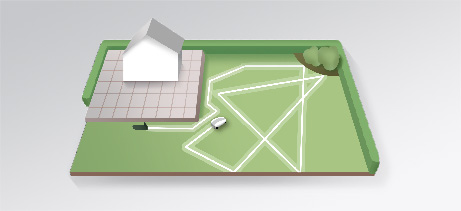
\includegraphics[scale=0.8]{figures/noLogiCut.jpg} 
\label{fig:randomcut}
\caption{Random cut system [source:Bosch]} 
\end{figure}

\noindent
When the battery is nearly discharged, the mower will follow the guard wire back to the base station for recharging.\\\\
\noindent
Parallel line mowers use a more intelligent control algorithm to optimize the mowing. After an initial learning run, following the guard wire around the lawn to be mowed, it will map the lawn, and cut in parallel lines, see \figref{fig:logicut}. The advantage of this strategy efficiency, as the lawn mower will not run over the same spots more than once. According to Bosch, a given lawn can be mowed up to 30\% faster with their Logicut system.
%% TODO: Insert source
 

\begin{figure}[H]
\centering
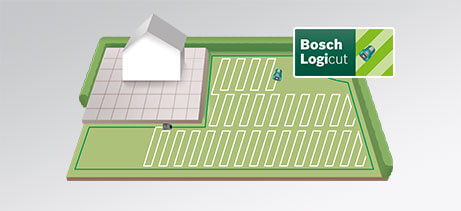
\includegraphics[scale=0.8]{figures/logicut.jpg} 
\label{fig:logicut}
\caption{Bosch Logicut system [source:Bosch]} 
\end{figure}

\noindent
Common for both systems is the guard wire, which has to be placed around the lawn and anywhere the lawn mower is not allowed to go, like flower beds, swimming pools, etc. \\\\
\noindent
This brings us to the problem with existing products.

\section{Problems with existing robotic lawn mowers}
All commercially available robotic lawn mowers requires a guard wire placed around the lawn. This can either be placed at the surface, and be held in place by pegs, or dug down below the surface. The guard wire must be routed around flower beds, etc. as well, see \figref{fig:robomow}

 
\begin{figure}[H]
\centering
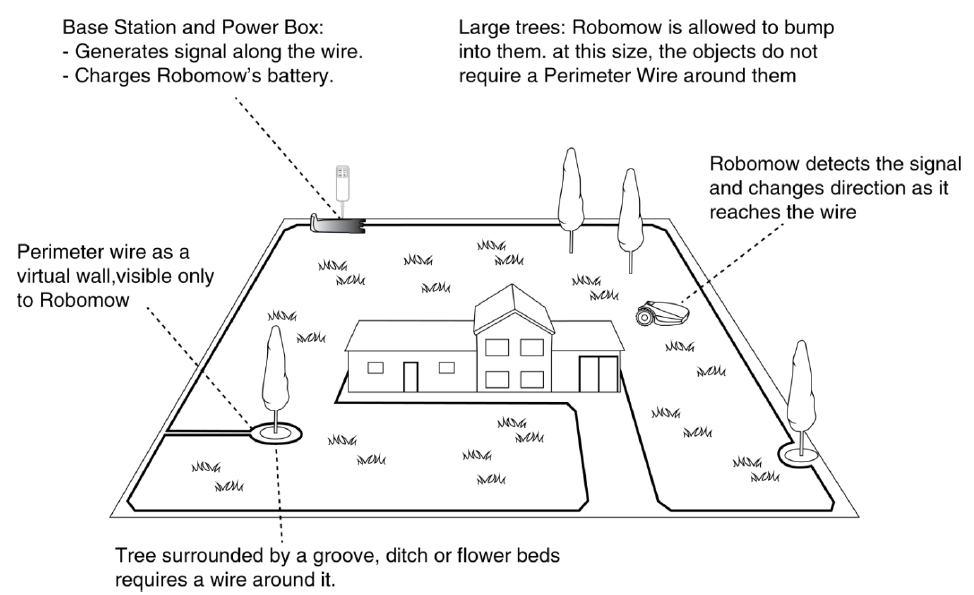
\includegraphics[scale=0.6]{figures/robomow.png} 
\label{fig:robomow}
\caption{Guard wire installation [source:Robomow]} 
\end{figure}
\noindent

The use of the guard wire for guiding the mower back to the charging station presents another potential problem: in a garden with many restricted areas, the guard wire could get very long. This could therefore make the journey home long, compared to a more direct route. This again uses more battery power, that instead could have been used for actually mowing the lawn.\\\\
\noindent
This will be the motivation for the project: to avoid the work routing a wire around the garden, and as a bonus get more work done on a battery charge, by not wasting power following the wire home.\\\\
\noindent
Then, the question is: What other solutions could be use to get the lawn mower to go where it has to go? \\
One first step could be to keep track of where it is in real-time.
%-- Section : GoT introductory presentation --%
\section{The Games on Track (GoT) system}
We were provided with the \emph{Games on Track GT-Position} system as a start to be able to determine the lawn mower's position in space. 
% Add reference to GoT description

\begin{figure}[H]
\centering
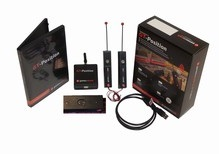
\includegraphics[scale=1.1]{figures/gotSystem.jpg} 
\label{fig:gotsystem}
\caption{Games on Track GT-Position package [source:Games\ on\ Track]} 
\end{figure}
\noindent

\noindent
It is composed of four different parts both hardware and software :
%% TODO : Add reference to http://www.gamesontrack.co.uk/pages/webside.asp?articleGuid=64556
\begin{itemize}
	\item A tracked module, which emits ultra-sound waves. It should be placed on the lawn mower itself while taking care, that the emitting cell is not obstructed by anything.
	\item Beacons or receivers, placed around the area the lawn mower will move in. Depending on the terrain, anywhere from 2 \todo{--Resolved-- is two enough? Answer: It is according to the GoT site (see reference in LaTeX comments)} to more than 20 of these can be used: the more is placed, the more accuracy can be obtained to fight against any ambient noise.
	\item The central system, which calculates the distance of the tracked module to each beacon, and transmits it to the computer via USB in regular intervals.
	\item The GoT software aggregates the received positions throughout time, and can be used to draw a map of the terrain (the lawn), and to determine the absolute position of the tracked module.
\end{itemize}

GoT was originally designed for train modelling, but it is easily adaptable for any use of position tracking and seems a good choice, at first, for our autonomous lawn mower.
But, why not use a satellite based positioning system ?

%-- Section : Satellite vs GoT --%
\section{Satellite based positioning systems vs GoT}
\todo{Wrong reasons for GPS vs GoT, elaborated below}
The reasons why satellite positioning system won't be used in our project are mainly related to accuracy over price ratios and to energy consumption.\todo{--To be reviewed again-- GPS uses very little power -> depending on the accuracy needed...}

\noindent
Indeed, these kinds of system like GPS or GLONASS would require a dedicated chip to put on the final system. The problem then would be the lack of precision. Although, there are some cheap standard GPS chips (around USD 10), these only reach around 1 meter of precision in the most ideal situations. % ref : www.gps.gov
On the other hand, the best GPS chips can achieve precisions up to a few millimeters when combined with different augmentation systems (algortihms for instance), but they end up being highly expensive (usually thousands of dollars). They are not generally intended for public use.
\todo{--To be reviewed again-- Only applies to cheap solutions, differential GPS can go to mm level, but is extremely expensive. This is what we are trying to replace with GoT, as it is a lot cheaper than diff-GPS} \\\\
%% TODO : Add reference to "A Review of GLONASS" Miller, 2000 & http://www.gps.gov/systems/gps/performance/accuracy/ 
\noindent
Moreover, if we add up the slow bit rates satellites can achieve, the signal amplifiers on the receiver, plus all the position calculations and possible augmentation systems, the total energy consumption would quickly rise,\todo{--To be reviewed again-- nope, it's just a radio receiver, uses almost no power} thus reducing the lawn mower autonomy, which is not desirable.\\
Indeed, the design of a product has no real value if no one is interested in using it. This is why choices made during this project have to be made in accordance with the final user's expectations.\\\\
\section{Potential consumer expectations}
Usually, we can think of a few priorities consumers will have when buying a product, whatever it is, and some more specific to technical products.\\
\noindent
Here for instance, the autonomy of the vehicle (both in energy and for the navigation), and the overall cost should be considered. The GoT system itself has a cost (USD 606.00 for a basic package) beyond anything a normal customer would probably pay for a lawn mower. But despite that, it appears, at first, to be a good solution for us in terms of accuracy and energy consumption compared to GPS-like systems which are even more expensive for the same accuracy. \todo{--Resolved-- insert price approximation here - not so true actually} \\\\
\noindent
These are the types of preliminary considerations that will influence this design process for an autonomous lawn mower.
\section{Robotic Lawn Mowers}\label{roboMowers}
Several manufacturers of electrical gardening machines have started selling robotic lawn mowers in the recent years. In general they use one of these two strategies when cutting the lawn \todo{Source}:
%
\begin{itemize}
	\item Random direction mowers.
	\item Parallel line mowers.
\end{itemize}
%
Mowers utilizing the random direction strategy will drive in a straight line until a guard wire or an obstacle is detected. They will then turn in a random direction, and continue. See \figref{fig:randomcut}.

\begin{figure}[H]
\centering
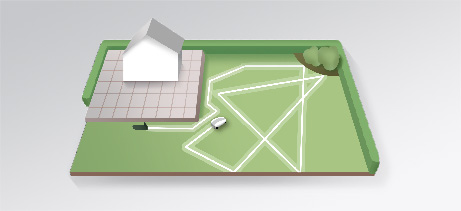
\includegraphics[scale=0.8]{figures/noLogiCut.jpg}
\caption{Random cut system \cite{Bosch}} 
\label{fig:randomcut}
\end{figure}
\noindent
When the battery is nearly discharged, the mower will follow the guard wire back to the base station to recharge.
%
Parallel line mowers utilize another control algorithm for mowing. After an initial learning run, following the guard wire around the lawn to be mowed, it will map the lawn, and cut in parallel lines, see \figref{fig:logicut}. The advantage of this strategy, is that the lawn mower will not run over the same spots more than once. According to Bosch, a given lawn can be mowed up to 30\% faster with their Logicut system \cite{Bosch}.

\begin{figure}[H]
\centering
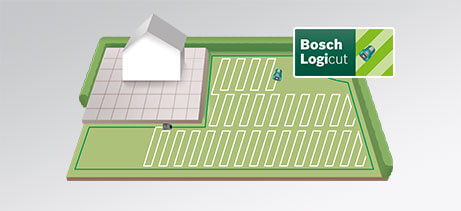
\includegraphics[scale=0.8]{figures/logicut.jpg} 
\caption{Bosch Logicut system \cite{Bosch}}
\label{fig:logicut}
\end{figure}
\noindent

Common for both systems is the guard wire, which has to be placed around the lawn and anywhere the lawn mower is not allowed to go, like flower beds, swimming pools, etc.
\subsection{Existing Problems}
Some commercially available robotic lawn mowers require a guard wire placed around the lawn. It can either be installed at the surface, and be held in place by pegs, or dug down below the surface\todo{source?}. The guard wire must be routed around flower beds, bushes etc. as well, see \figref{fig:robomow}.\\\\
%
The use of the guard wire for guiding the mower back to the charging station presents another potential problem: in a garden with many restricted areas, the guard wire could get very long. Therefore the journey home could be longer, compared to a more direct route. This again uses more battery power, that could have been used for actually mowing the lawn instead.\\\\
%
This will be the motivation for the project: to avoid the work routing a wire around the garden, and as a bonus get more work done on a battery charge, by not wasting power following the wire home.\\\\

\begin{figure}[H]
\centering
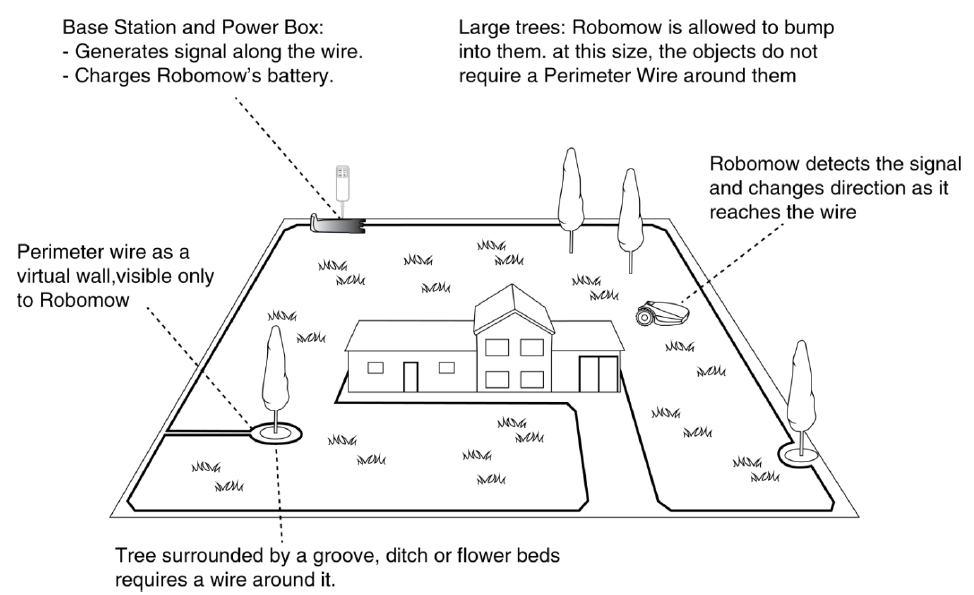
\includegraphics[scale=0.6]{figures/robomow.png} 
\caption{Guard wire installation [source:Robomow]}
\label{fig:robomow} 
\end{figure}
\noindent

Then, the next question is: what other solutions could be used to get the lawn mower to go where it has to go?
A solution of keeping track of the lawn mower's position in real-time is examined.
%-- Section : GoT introductory presentation --%
\section{The Games on Track System}
One available system is the \emph{Games on Track GT-Position} system, referred to as GoT. The GoT would be able to determine the lawn mower's position in space, see \secref{sec:Vehicledescription}. It is composed of three different parts both hardware and software \cite{GoTWebsitePos}:

\begin{itemize}
	\item A tracked module, which emits ultra-sound and radio waves. It should be placed on the lawn mower itself.
	\item Towers which are tracking the tracked module placed on the vehicle are needed. These should be located around the area where the lawn mower will move. There should be at least 3 towers, depending on the terrain, and can be up to more than 20. The more towers, the more accuracy can be obtained to cancel out any ambient noise, and more space can be monitored.
	\item The master, connected to a computer, receives data from the towers and transmits it to computer through a USB in regular intervals. The distance of the tracked module is then calculated by the computer.
\end{itemize}

\begin{figure}[H]
\centering
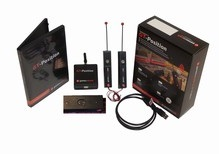
\includegraphics[scale=1.1]{figures/gotSystem.jpg} 
\caption{Games on Track GT-Position package [source:Games\ on\ Track]} 
\label{fig:GoTsystem}
\end{figure}
\noindent
%
The GoT software aggregates the received positions through time, and can be used to draw a map of the lawn, and to determine the absolute position of the tracked module.

GoT was originally designed for train modelling, but it is easily adaptable for any use of position tracking. In the following segment satellite based positioning systems are compared to the discussed GoT system.
%-- Section : Satellite vs GoT --%
\section{Satellite based positioning systems vs GoT}
\todo{Wrong reasons for GPS vs GoT, elaborated below}
The reasons why satellite positioning system won't be used in our project are mainly related to accuracy-over-price ratios and to energy consumption.\todo{--To be reviewed again-- GPS uses very little power -> depending on the accuracy needed...}\\\\
Indeed, these kinds of system like GPS or GLONASS would require a dedicated chip to put on the final system. The problem then would be the lack of precision. Although, there are some cheap standard GPS chips (around USD 10), these only reach around 1 meter of precision in the most ideal situations \cite{GPSUSWebsiteAccuracy,Miller}. \\
On the other hand, the best GPS chips can achieve precisions up to a few millimeters \cite{GPSUSWebsiteAccuracy} when combined with different augmentation systems (algortihms for instance), but they end up being highly expensive (usually thousands of dollars). They are not generally intended for public use.
\todo{--To be reviewed again-- Only applies to cheap solutions, differential GPS can go to mm level, but is extremely expensive. This is what we are trying to replace with GoT, as it is a lot cheaper than diff-GPS} \\\\
%
Moreover, if we add up the slow bit rates satellites can achieve, the signal amplifiers on the receiver, plus all the position calculations and potential augmentation systems, the total energy consumption would quickly rise, \todo{--To be reviewed again-- nope, it's just a radio receiver, uses almost no power} thus reducing the lawn mower autonomy, which is not desirable.\\\\
%
Indeed, the design of a product has no real value if no one is interested in using it. This is why choices made during this project have to be made in accordance with the final user's expectations.

%---------- Chapter 2 ---------------------------------------- Design Considerations
\chapter{Design Considerations}
\vspace{-5 mm}
In this chapter the system is designed with a top-down approach, which means an overview of the system is formulated first. Thereafter the system will be broken down into smaller segments. First a use-case model of the system, where the functionalities and the coherent actors is described, in order to give an overview of what the system must be able to do. Thereafter, constraints set by time limitations as well as a focus on the main scope of the project, in regards to the prototype, are considered.
\vspace{-4 mm}
\section{Use-case Design} \label{sec:UseCase}
To give an overview of what the system should be able to do, a use case with coherent actors is utilized. The use case diagram, see \figref{fig:usecase}, will describe the main functionalities in the use case as well as describing the actors, the external sensors and systems, affecting the system.

%The use-case diagram is made, where the micro controller is the system that will be analysed, because, it will be the master in this system

\vspace{-3 mm}
 \begin{figure}[H]
	\centering
	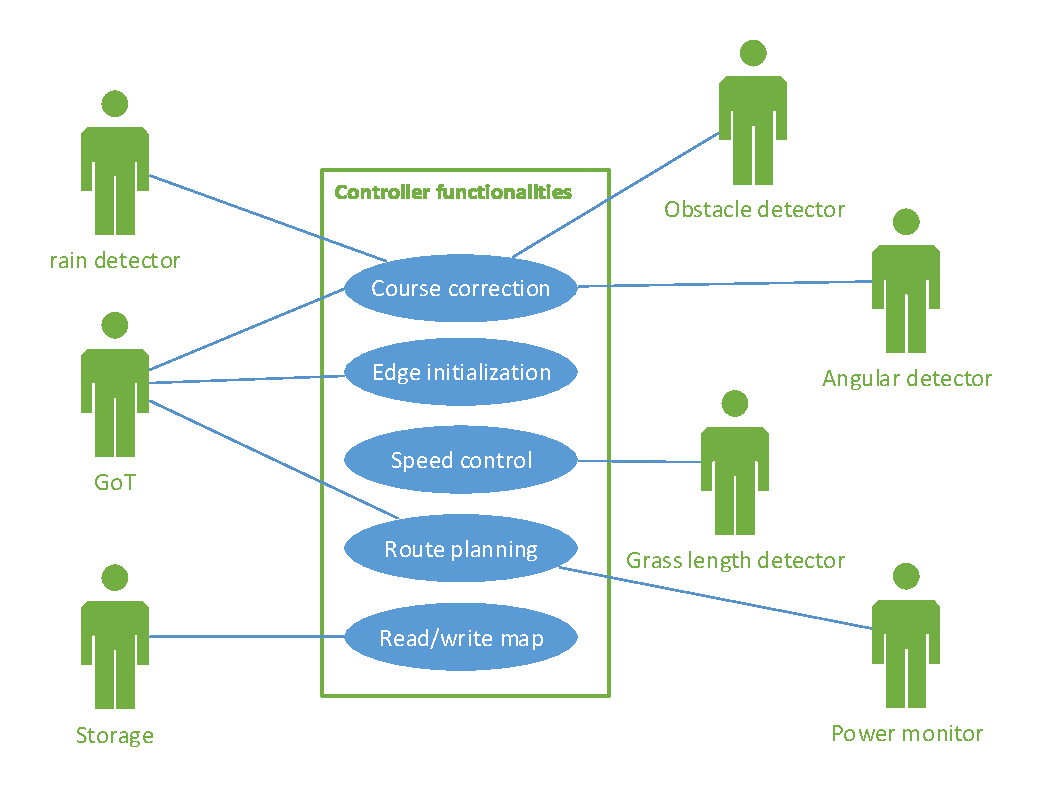
\includegraphics[scale=0.8]{figures/P5UseCase.pdf}
	\caption{Use-Case Diagram}
	\label{fig:usecase}
\end{figure}

\noindent
\newpage

The system, inside the controller, have 6 main functionalities and is affected by 9 different actors.

\subsection{Main Functionalities}

Functionalities are the functions that the system can do. Each Functionality can have more than one function in the system. The functionalities get input from actors and can be in association with other functionalities. 

\textbf{Edge Initialization}:
The \textit{Edge Initialization} gets input from the \textit{GoT} system and is associated with the \textit{Read/Write Map} functionality. The purpose of this function, is to calibrate the system to a new lawn, by mapping the edge of the lawn. The edges which is mapped should include the area in which the vehicle should stay inside and the areas which it should avoid, e.g. trees, bushes and so on. This is done, by first manually moving the \textit{GoT} system's transmitter along periphery of the lawn and thereafter along the edges of obstacle placed on the lawn. This could be performed by the use of a button which could make the system record edges if pressed. The information about the edges, an edge map is created and saved through the \textit{Read/Write Map} function.

\textbf{Route Planning}:
The \textit{Route Planning} gets input from the \textit{Power Monitor} and is associated with the \textit{Read/Write Map} functionality. The purpose of this function, is to plan the route for the lawn mower. The route is created by knowing where the lawn mower is located and the map of edges of the lawn, which is located in \textit{Storage}. The map is loaded from the \textit{Storage} with the \textit{Read/Write Map} function. Furthermore it acquires the voltage level of the battery from the \textit{Power Monitor}, to ensure it will return to base before it runs out of battery.

\textbf{Read/Write Map}:
The \textit{Read/Write Map} gets input from the \textit{Storage} and is associated with the \textit{Route Planning}, \textit{Course Correction} and the \textit{Edge Initialization} functionalities. This functionality is the link between functionalities and \textit{Storage}. The edge map retrieved from \textit{Edge Initialization} and through use of the \textit{Read/Write Map} function, is stored in the \textit{Storage}. In \textit{Storage}, the route which calculated by the \textit{Route Planning} is also located. The \textit{Course Correction} functionality also needs access to the \textit{Storage} to be able get the calculated route.

\textbf{Course Correction}:
The \textit{Course Correction} gets input from the \textit{GoT} system, the \textit{Humidity Detector}, the \textit{Obstacle Detector} and the \textit{Angular Detector} and is associated with the \textit{Read/Write Map} and the \textit{Speed Control} functionalities. This function gets both an angle and the humidity in the air as input, furthermore it gets an input if it encounters an obstacle blocking its path. \textit{Course Correction} takes all these parameters into consideration when navigating from its last registered position, retrieved from the \textit{GoT} system, to the next destination on the calculate route retrieved from the \textit{Storage} trough \textit{Read/Write Map}. The \textit{Course Correction} is the main function behind the regulation of the vehicle's angular movement. The  \textit{Course Correction} decides the velocity, according to the calculated route, and passes the decided velocity to the \textit{Speed Control}.

\textbf{Speed Control}:
The \textit{Speed Control} gets input from  the \textit{Grass Length Detector} and the \textit{Speed Measurement} and is associated with \textit{Course Correction}. The function's purpose, is to make sure that the lawn mower adapts the speed depending on the grass length and if the \textit{Course Correction} ask for a different velocity, e.g. if the vehicle is going into a curve.

\textbf{Blade Control}:
The \textit{Blade Control} gets input from the \textit{Blade Monitor}. The function's purpose, is keeping the blade rotational speed the same, to make an even cut grass. With the input from the \textit{Blade Monitor}, the \textit{Blade Control} can regulate the velocity of the blade.

\subsection{Actors}
A actor is a component, that influence the system by giving inputs to the functionalities and/or receiving outputs from them.

\textbf{GoT}:
The \textit{GoT} system is connected to the \textit{Course Correction}, the \textit{Route Planning} and the \textit{Edge Initialization} functionalities. This system is used to retrieve the GoT transmitter's, placed on the vehicle, location on the lawn. The GoT system is explained in \appref{GoTDescription}.

\textbf{Storage}:
The \textit{Storage} is connected to the \textit{Read/Write Map} functionality. It uses a non-volatile storage to store the information about the edge map and route, which is made in the \textit{Edge Initialization} and \textit{Route Planning} functionalities. This will make the \textit{Storage} able to keep the data even if the system is turned off.

\textbf{Humidity Detector}:
The \textit{Humidity Detector} is connected to the functionality \textit{Course Correction}. This is a sensor that measures the humidity in the air. The system uses the information about the ambient humidity level to see, whether the grass is too wet for mowing the lawn, since wet grass can not be cut evenly. 

\textbf{Obstacle Detector}:
The \textit{Obstacle Detector} is connected to the \textit{Course Correction} functionality. This sensor detects, if there are any objects, which blocks the lawn mower's route. This sensor makes sure, that the lawn mower registers objects, like a human or a dog, which could interfere with the lawn mower's route.

\textbf{Angular Detector}:
The \textit{Angular Detector} is connected to the \textit{Course Correction} functionality. This sensor measures the angular position and movement of the lawn mower, whether it is intentional movement or if the lawn mower slips.

\textbf{Grass Length Detector}:
The \textit{Grass Length Detector} is connected to the \textit{Speed Control} functionality. This sensor measure the  grass length, which affects the velocity, at which the lawn mower should drive. If the grass is long, the lawn mower has to drive slower, to make sure that it cuts the grass evenly. 

\textbf{Power Monitor}:
The \textit{Power Monitor} is connected to the \textit{Route Planning} functionality. This sensor measures how much power is left in the battery. This is needed, so that the lawn mower can drive back to its charging station, before the battery is too low, to not destroy the battery.

\textbf{Blade Monitor}:
The \textit{Blade Monitor} is connected to the \textit{Blade Control} functionality. This sensor measures the rotational speed of the blade and send the information back to the \textit{Blade Control}

\textbf{Speed Measurement}:
The \textit{Speed Measurement} is connected to the \textit{Speed Control} functionality. The sensor measure the speed of the lawn mower.
%
\section{The Vehicle}

\subsection{The vehicle in general}


\subsection{Drivetrain}
The drivetrain of a motored vehicle, is the components that transfer the rotational energy from the motor to the drive wheel of the vehicle. For this vehicle, the drivetrain will contain the gear connected to the brushed DC motor, the differential gear box and the gears connected to the belts. The drivetrain is illustrated in \figref{vehicleDescriptionDriveTrain}.

\begin{figure}[H]
	\centering
	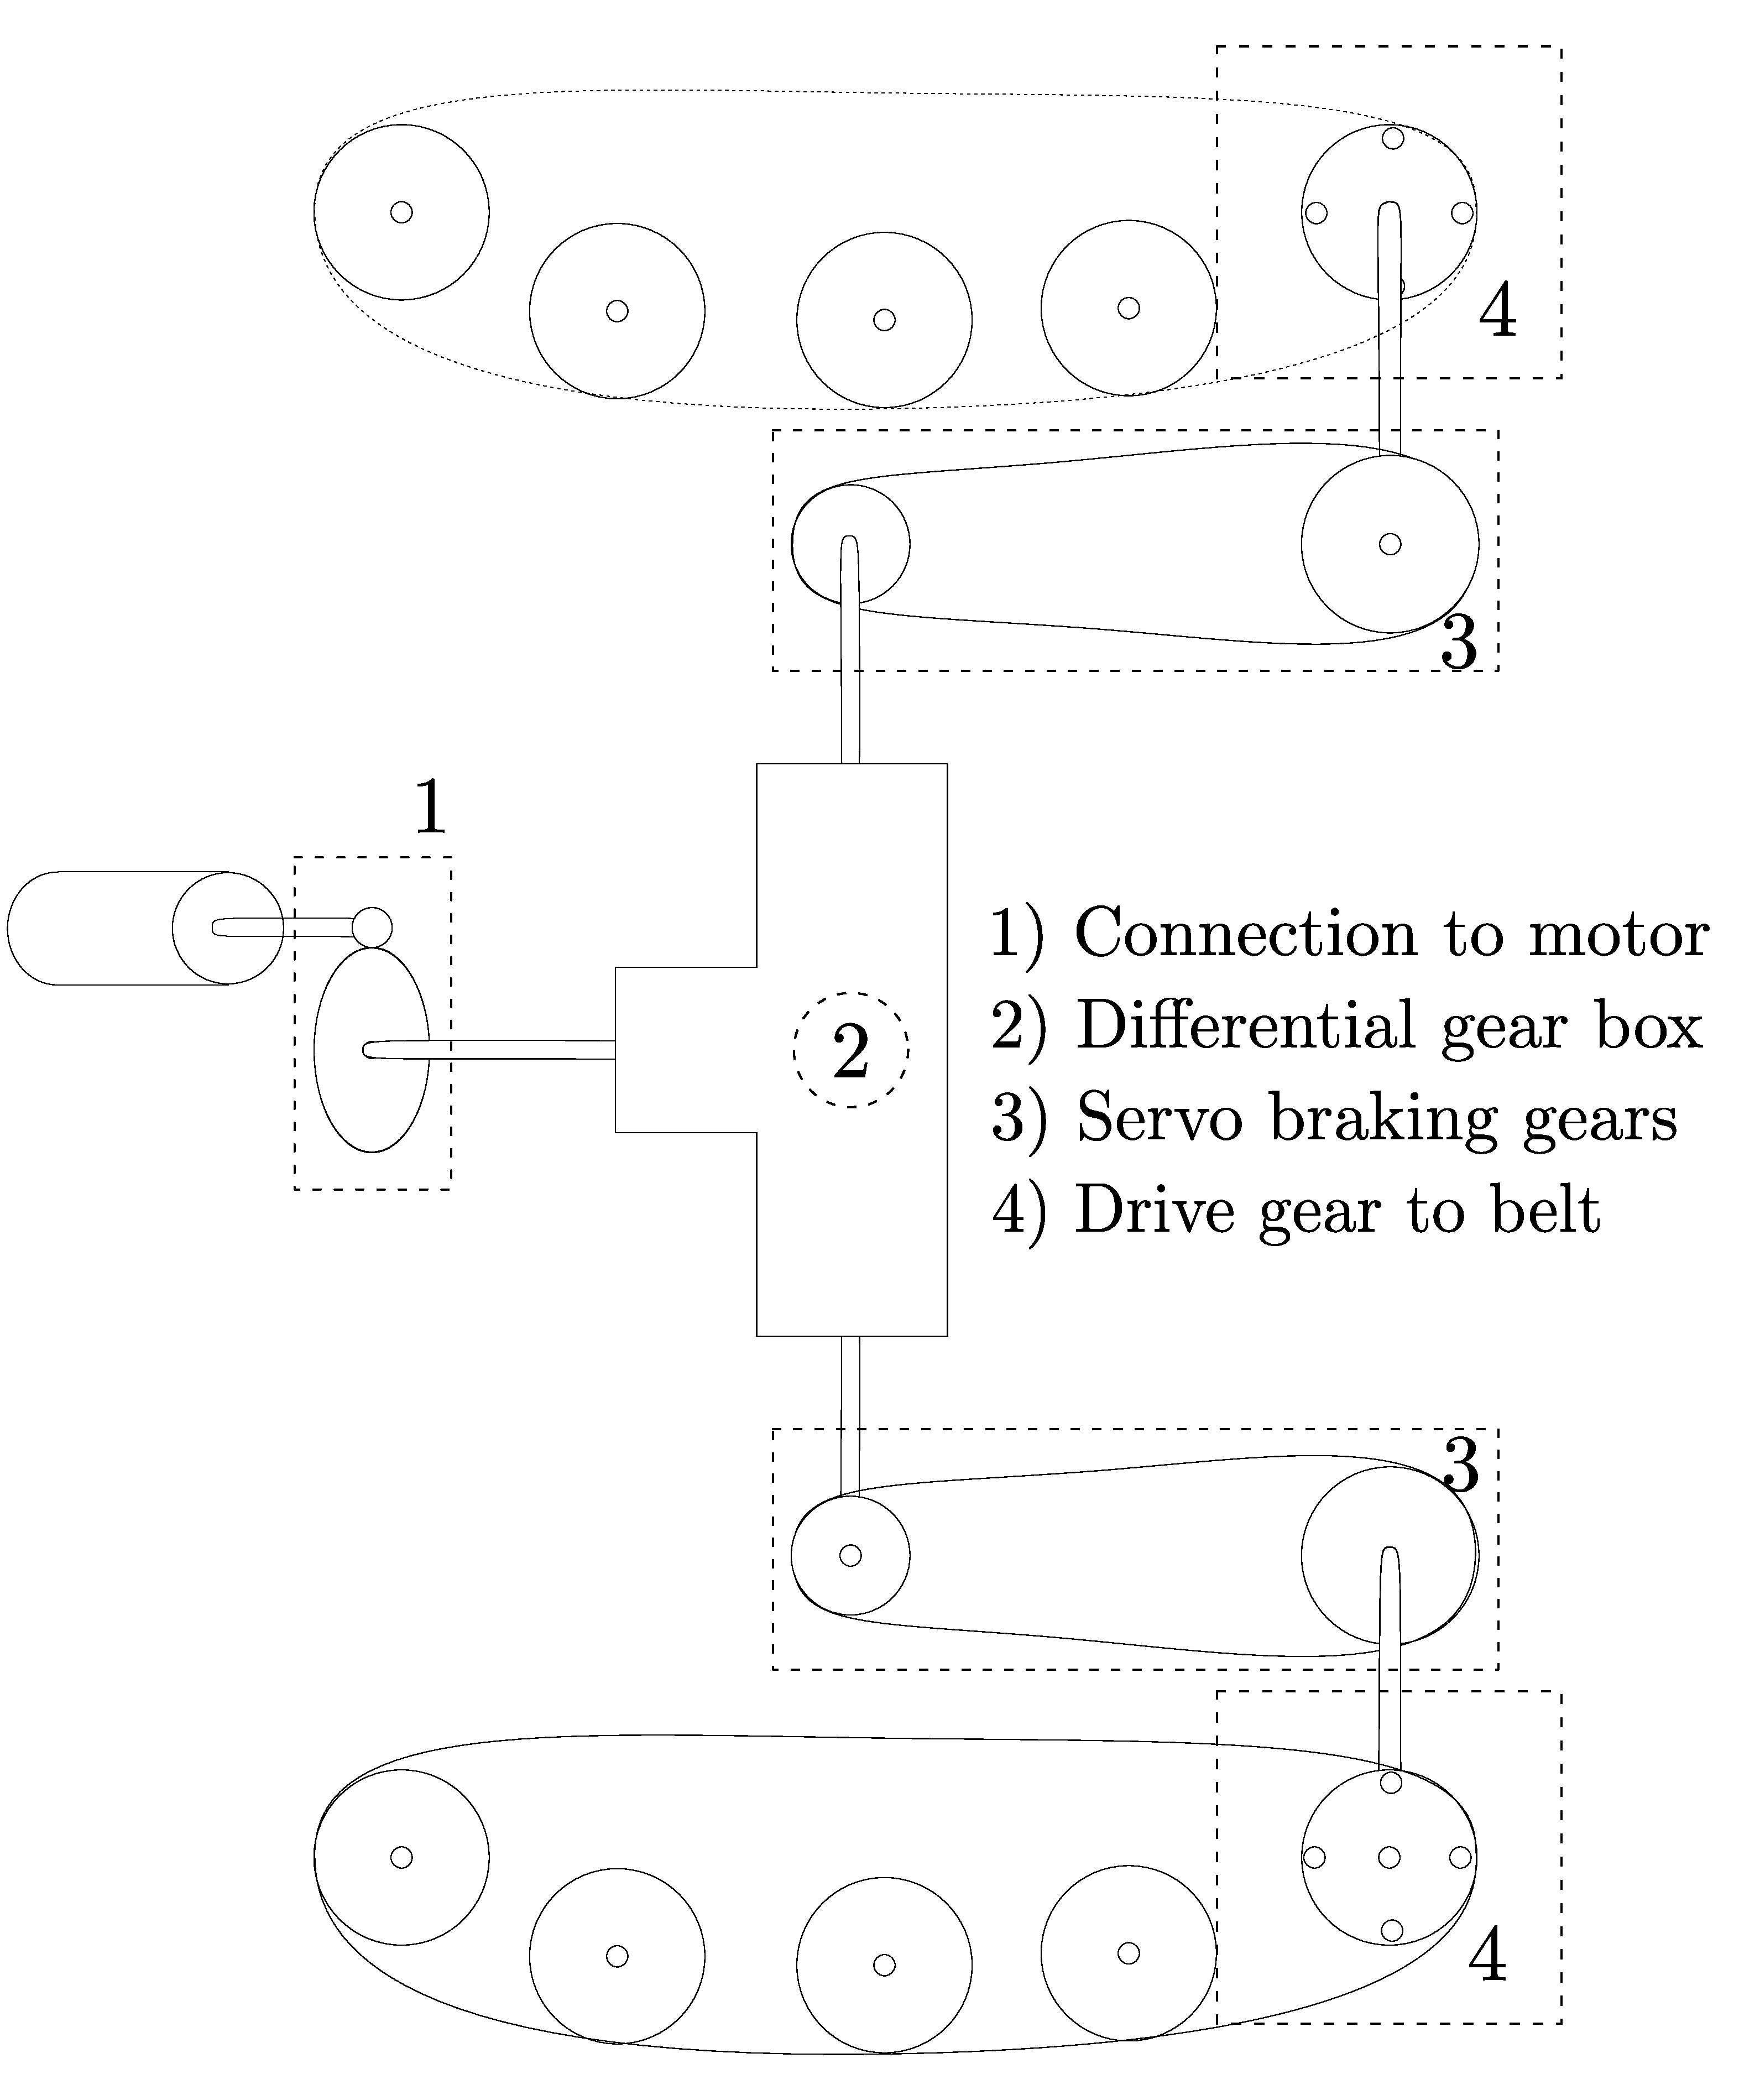
\includegraphics[scale=1]{figures/vehicleDescriptionDriveTrain.pdf}
	\caption{Illustration of the drive train of the vehicle.}
	\label{vehicleDescriptionDriveTrain}
\end{figure}

The motor delivers a force to the system through a the motor-shaft with a connecting gear. This gear is connected to the start of the drivetrain(1). From there the differential gear box is connected(2). From the differential gears two shafts are connected to a gear which transfers the velocity to the drive wheels(3).
From there the rotational velocity makes the drive-wheel turn, thus rotating the belts which are supported by four free wheels on each side(4). 

The following sections will describe the different parts of the drivetrain seen on \figref {vehicleDescriptionDriveTrain}.\\ \todo{her er Amalie og Niels nået til}            %----Drivetrain
\subsection{Differential gears} \label{sec:Differentialgears}

When the servomotor is braking, it triggers the differential gears to make the vehicle turn.\\
Differential gears are used to reduce slipping between opposite wheels when a car is turning. The system can not avoid slipping under the tracks because they are too long, they will rotate at least around the center of the track. However, using differential gears will help control the course of the vehicle by transfering the power of the braking track to the other track.\\

As seen on \figref{diffGearLight}, the power is transmitted from the pinion gear (not represented on this picture) to the spider gear (here in green) fixed on the ring gear (here in blue). Only the spider gear is connected to the side gears(here in pink and yellow), fixed to the wheels.\\

\begin{figure}[H]
	\centering
	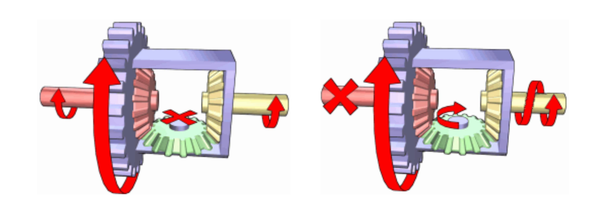
\includegraphics[scale=0.7]{figures/diffGearLight}
	\caption{Transfer of the power to the side gear when the spider gear is blocked versus when it spins \cite{MechanicalEngineering}}
	\label{diffGearLight}
\end{figure}

When the ring gear is turning but the spider gear does not spin, both side gears turn the same speed. But if one side gear is blocked, the spider gear will spin,  and the other side gear will turn faster.\\

There are usually two spider gears (here in red) for more reliability and solidity, and the ring gear (here in blue) is set in motion by the pinion gear (here in brown in front) as seen on \figref{diffGearFull}.\\

\begin{figure}[H]
	\centering
	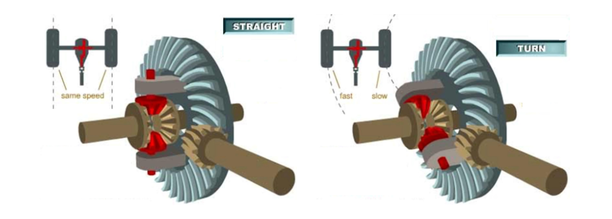
\includegraphics[scale=0.7]{figures/diffGearFull}
	\caption{Description of the differential system going straight vs turning \cite{MechanicalEngineering}}
	\label{diffGearFull}
\end{figure}

This is the element the servo is using when braking one track, allowing the other track to turn still.\\\\



The description of the vehicle allows then to consider a prototype of the functionnalities needed in this project.



\subsection{Brakes}

 \begin{figure}[H]
	\centering
	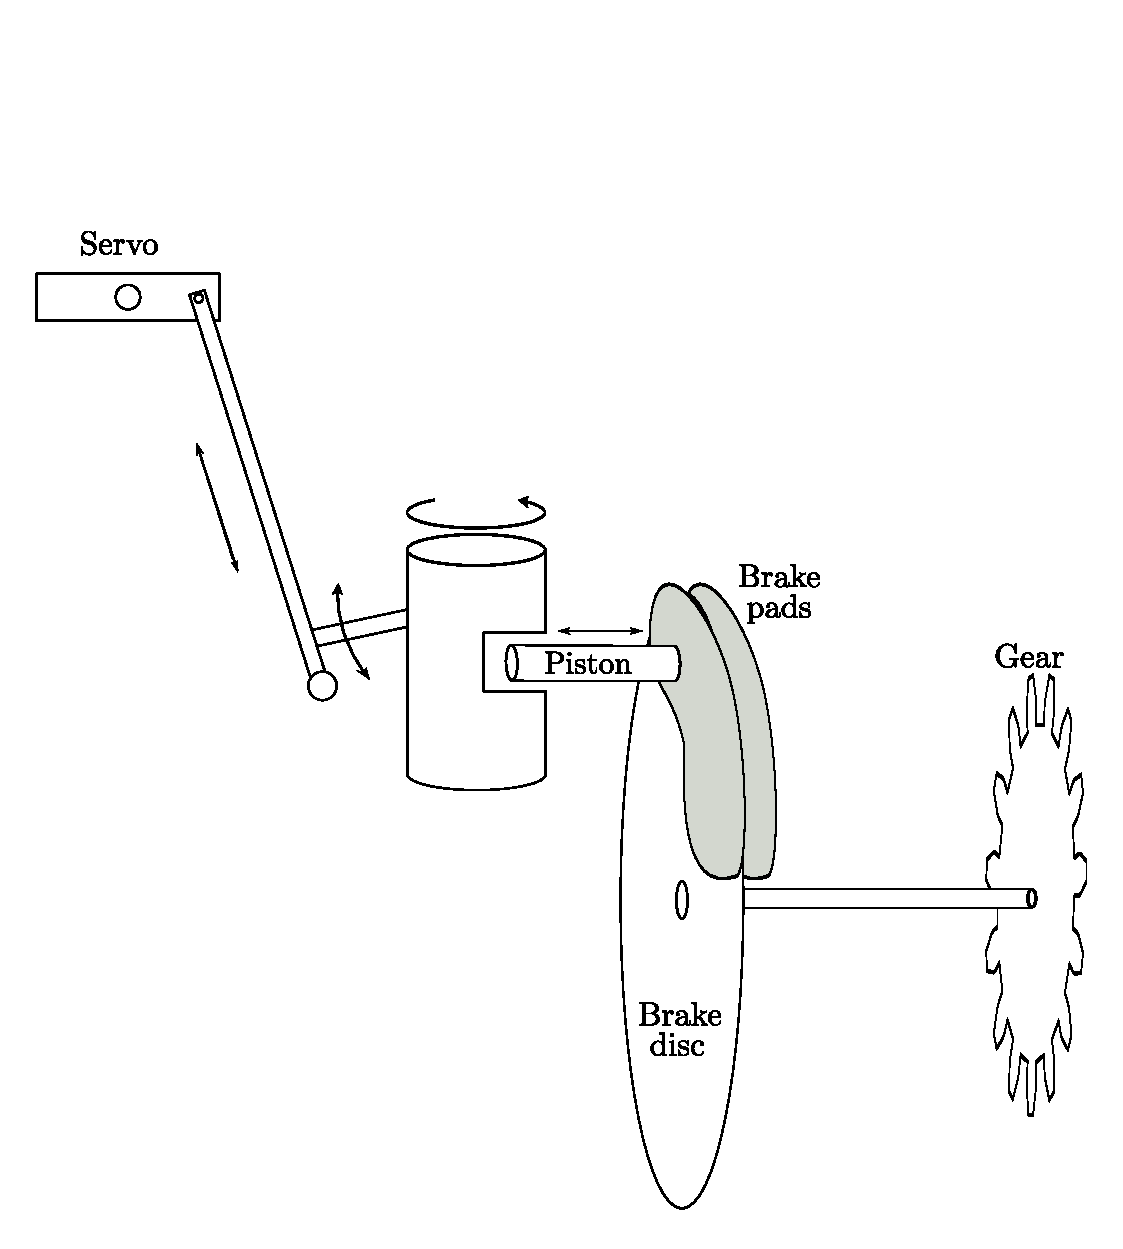
\includegraphics[scale=0.6]{figures/brakeDescription.pdf}
	\caption{Illustration of the brakes}
	\label{Brakes}
\end{figure}                %---- Steering
\subsection{Servo}
On the vehicle there is a servo, which is a S3003 by Futaba.
The servo is used for the steering of the vehicle. The servo controls the steering through breaking one of the belts and transfer that power over to the other belt.


The Servo is controlled by a PWM signal. The PWM signal recieved is converted into an angle by the servo to control the steering of the belts, as seen on \figref{timeVSangle}. An angle of 90° is the normal position for going straight, while 0° and 180° are the limits for turning, where one of the belts is not moving. 

A mechanical arm is mounted on the servo and connected to the brakes of the tracks. When the servo rotates one way, it triggers the brakes more on one side and less on the other side, according to the value of the angle sent, through the PWM signal. This way, one of the belt will drive slower and the other belt drive faster, which will make the vehicle turn, without decreasing the motor power.

The servo reacts lineary to the PWM signal and the cycle of the signal is 30 milliseconds. To get the servo to be in neutral position, the servo needs a PWM signal of 4.83 \% (a period of 1450 microseconds). For 180°, it is 8.33 \% (a period of 2500 microseconds) and 1.67 \% (a period of 500 microseconds) for 0°. \\

%source http://www.societyofrobots.com/actuators_servos.shtml\\

\begin{figure}[H]
	\centering
	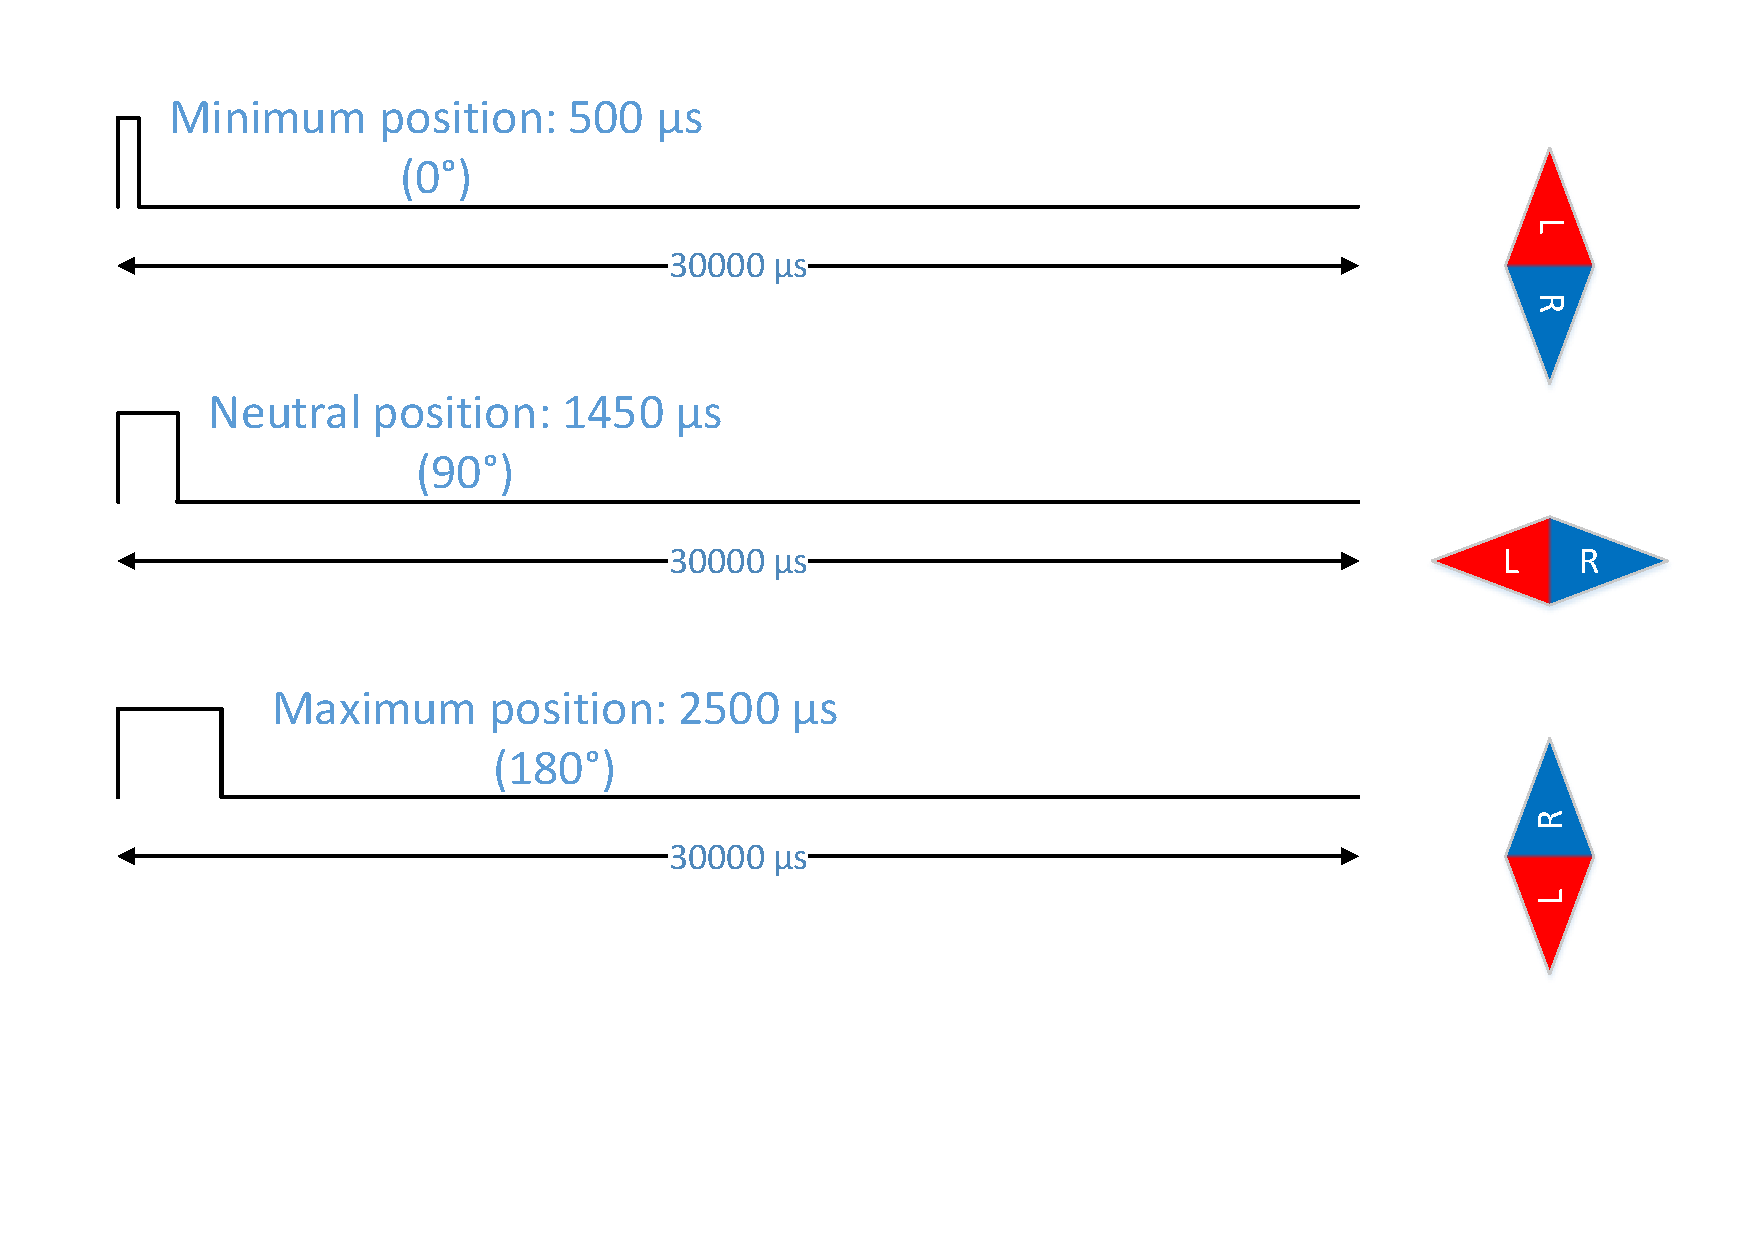
\includegraphics[scale=0.6]{figures/TimeVSangle.pdf}
	\caption{Convertion from time to angle by the servo}
	\label{timeVSangle}
\end{figure}


\subsection{Hall Sensor}
There are two hall sensors implemented on the vehicle, one by each drive gear, illustrated in \figref{vehicleDescriptionDriveTrain}. Four magnets are placed on each drive gear, with a quarter turn between each. The Hall sensor is illustrated in \figref{HallSensor}.

\begin{figure}[H]
	\centering
	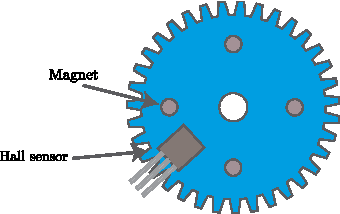
\includegraphics[scale=1.2]{figures/hallSensorDrawing.pdf}
	\caption{Illustration of the drive gear, with the magnets and the Hall sensor. The Hall sensor is placed stationary beside the rotating gear \cite{KHSoerensen}.}
	\label{HallSensor}
\end{figure}\vspace{-5mm}
%
A Hall sensor is affected by magnetic fields. When the field is significantly larger than the ambient fields a pulse is generated. This gives a voltage output each time one of the magnets is in front of the Hall sensor. Therefore each time the drive gear makes a quarter of a turn a voltage signal is generated.

%As the distance between each magnet is not exactly a quarter of a turn, the calculations of the pulses received from the Hall sensor, is processed for each magnet independently.
%By measuring the time between five outputs, as the first and the fifth output is from the same magnet, the time of a whole rotation of the gear can be found. By knowing the distance the vehicle travels for a full rotation of the gear, the speed can be calculated.
%
%When the vehicle is starting to move, the speed of the first turn of the gear can not be calculated. This is because two signal from the same magnet are needed before the speed can be calculated. So the first four output from the hall sensor will be saved and at the fifth output, after a whole turn, the speed related to the first magnet will be calculated.\\
%
%The hall sensors are used to measure the speed of the two belts, which will run at different speeds when the vehicle is turning. Now that the components linked to the velocity  are described, the steering material will be analysed.
            %---- Hall Sensor
\subsection{Battery Pack Specifications} \label{sssec:BatterySpecs}
In order to power the motor, the servomotor, and all the electronics, an electrical power source is needed. A NiMH battery pack from Ansmann Racing with \si{7,2\ V} nominal voltage and a \si{4700\ mAh} capacity is given with the vehicle \cite{BatteryDS}. The charge voltage cannot go beyond \si{9,0\ V} and should stay above \si{6,0\ V}.

The provided vehicle and battery have been described. Now it is necessary to understand how the GoT system works, to be able to utilize it to track the vehicle. 			%---- Battery Specifications
\subsection{GoT Description}
\label{GoTDescription}
The Games on Track GT-Position system, shortened GoT, is a positioning system which uses radio-waves for communication and ultrasound to locate a tracked object in space. The system has a sampling rate of 10 \si{Hz}, but it can vary a little because of ultrasound waves propagation. The system is built up from three types of hardware components: the transmitter, the satellites and the master, see \figref{GoTSystem}. The transmitter and the satellites send the information in all directions, with 360 degrees range signals.\\
The GoT System does not work if the transmitter is not close enough to the satellites. Furthermore, it can be disturbed if there are some interference by another ultrasound signal or by an object between the satellites.
%
\begin{figure}[H]
	\centering
	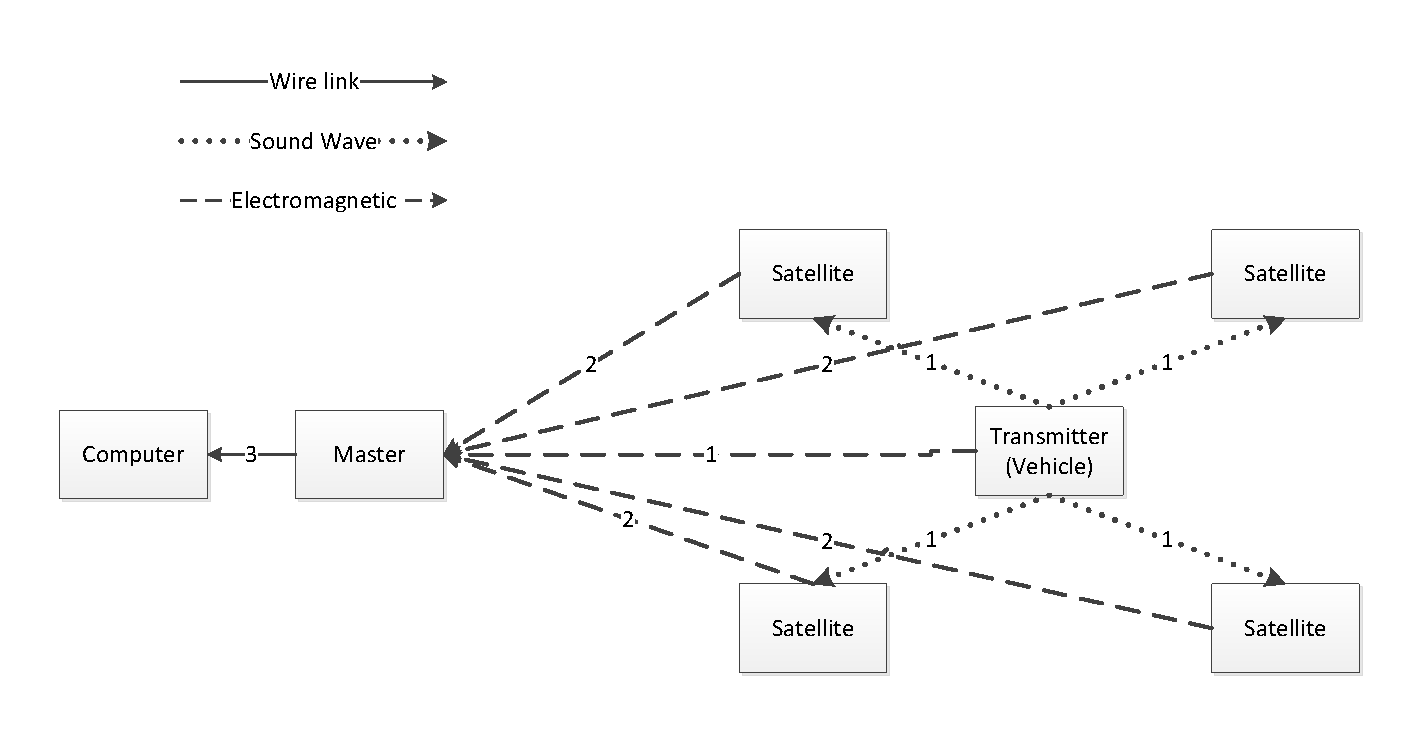
\includegraphics[scale=0.7]{figures/GoT_description.pdf}
	\caption{Overview of the GoT system, and the placement of hardware components.}
	\label{GoTSystem}
\end{figure}
%
\subsubsection{Transmitter}
The transmitter component is placed on the object which needs to be located. The transmitter sends an ultrasound burst out containing an identification number, that the satellites are intended to receive. The time at which each ultrasound bursts are sent from the transmitter to the satellites is transmitted by radio waves to the master. An ultrasound burst is sent each tenth of a second, giving a sampling frequency of 10 Hz.\\ 
The transmitter component runs on 2 AA-batteries and therefore does not need an external power-source.
%
\subsubsection{Satellites}
The satellites components are placed around the area where the object, with the transmitter on it, has to be located. The satellites' assignment is to search for the ultrasound waves, which the transmitter emits, and send a radio wave signal to the master as soon as they receive the burst.

To be able to calculate the exact position of the transmitter and then the object, a minimum of three satellites is necessary. However, more can be added to the system for more reliability, accuracy or to cover a larger area. To work with high efficiency, they should be placed each 1 to 2 meters apart from each other and not on a single line. But to cover a bigger area, they can be placed up to a distance of 5 meters between them, although this would affect the measurement and thereby make it less reliable. Each satellite has a maximum range of 8 meters and the three satellites should be placed in each other's reach. The satellites need between 14 to 20 volts DC, thus making the satellites able to be powered through a computer charger or by a panel solar for example is necessary.
%
\subsubsection{Master}
The master is a receiver which is connected to a computer. The master's assignment is to receive the data transmitted from the individual satellites and the transmitter, and to relay it directly to the connected computer. The master is powered through a USB cable, between the master and the computer.
%
\subsubsection{Computer}
The program on the computer, which is running in C\# and handles the information received from the master, uses the data to calculate the position of the transmitter. This is done with a method call trilateration. Trilateration is a way of calculating a position in a three-dimensional space, from three distances of known locations, with the help of spheres, circles and triangles as seen on \figref{GoTTriVSLine}.
%
\begin{figure}[H]
  \centering
 	%Trim margins @:   left        bottom       right       top
 	\adjustbox{ trim = {.01\width} {.15\height} {.01\width} {.01\height}, clip }
  {
    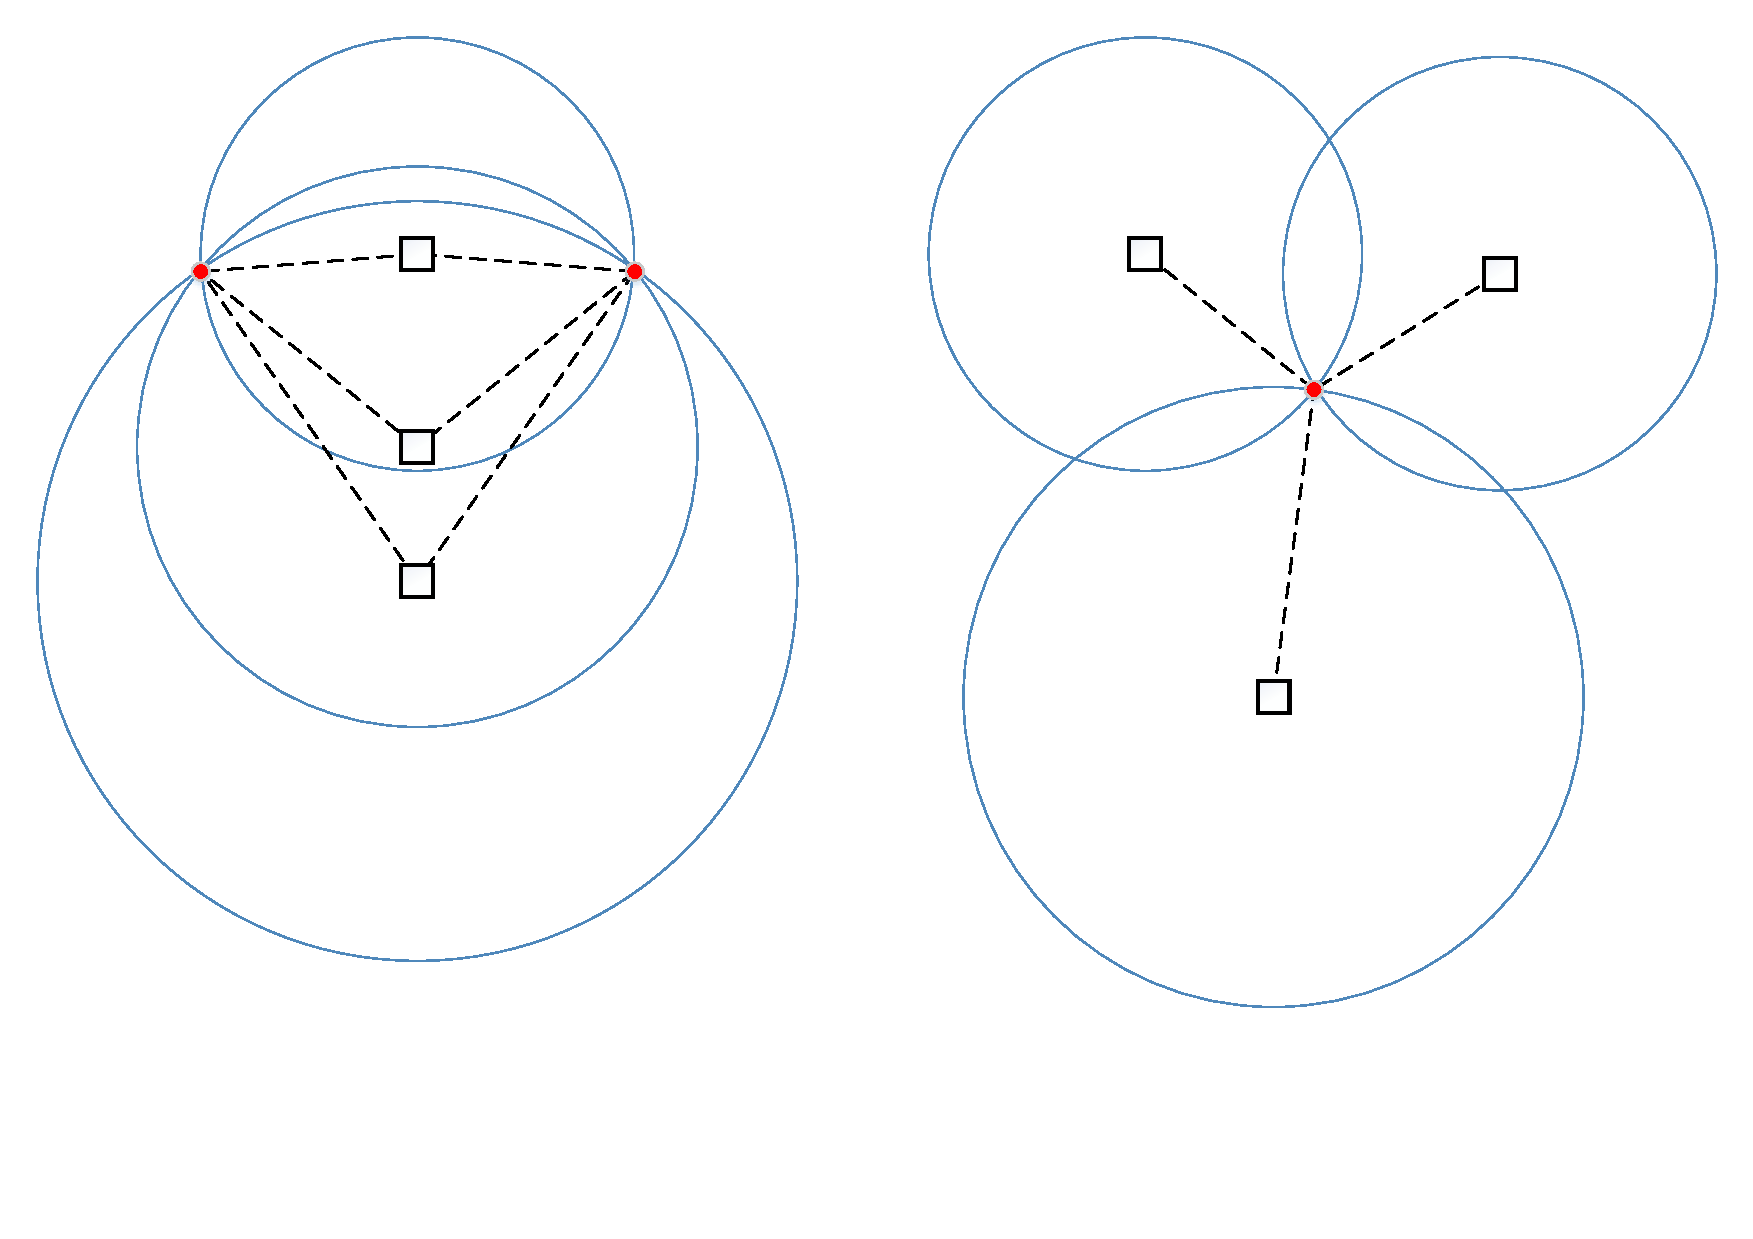
\includegraphics[width=0.9\textwidth]{figures/GoT_SingleVsTriangle.pdf}
  }
  \caption{To the left, satellites are aligned and will give two possible positions. To the right, satellites are placed in a triangle and will give one possible position}
  \label{GoTTriVSLine}
\end{figure}
%
If the satellites have been moved, it is necessary to recalibrate the system. This is done with a calibration triangle. The calibration triangle is made of three points on a flat surface and have a distance of 40 to 200 centimeters between them. One of the points on the calibration triangle is made the origin (0,0,0) of the new coordinate system. Another point on the triangle will then be called (X,0,0), in which the line between the first point and the second point will become the X-axis. The last point will be call (X,Y,0) and will determine in which way the positive Y-axis will go. The surface which the calibration triangle is placed on, will be the XY-plan, where Z will go vertically, defining the (X,Y,Z) coordinates. Thereafter, the transmitter is placed in the three point, with (0,0,0) first and (X,Y,0) last. When the transmitter is placed in a point, the satellites measure the distance between them and the transmitter. From this information, the program can calculate the position of each satellites, with the help of trilateration.

These are the basic elements from which the prototype is built. However, the functionalities suggested in \secref{sec:UseCase} need to be refined for the prototype implementation.
\section{Prototype Constraints}\label{sec:PrototypeConstraints}
Before the prototype can be established, some considerations have to be made in respect to time limitations and the main scope of this semester. The aim of the project is to create a functional automated proof of concept lawn mower. The following section provides argumentation for eliminated functionalities from the use case \secref{sec:UseCase}.

\subsection{Grass Length Detection}
Detection of the grass length to control the velocity of the lawn mower thus ensuring an evenly cut lawn, is a submodule which can be added at any time. Since it is not fatal for a working system and might even be unnecessary depending on time between each mowing of the lawn, it is decided to exclude this functionality from the initial design.

\subsection{Humidity Sensor}
As the lawn mower is supposed to work outside, it is important to consider that the grass could be humid. Since it is difficult to cut wet grass, a humidity sensor could be used to warn the system of the humidity, thus the system could go back to the charging station. This submodule is not fatal for a functional prototype, so this type of sensor will not be included in the design.

\subsection{Obstacle Avoidance}
The lawn movers path might not always be clear, e.g. garden tools, tables or moving objects could be in the way. The vehicle should be aware of what is in front of it at any time, to correct its path and be able to get around the obstacle if necessary. To avoid this the sensor could be a pushing button to detect a solid object or an ultrasound detector if the object is fragile.
As the aim of the project is to control the path of the vehicle by using angular positioning sensors, a proximity sensor will not be included. Static objects could be registered on the map to avoid these issues.

Furthermore the edge mapping functionality will not be included in the project which instead will focus on a map predefined in the test room.

%\subsection{Power Monitoring}
%Power monitoring could be implemented by measuring the voltage across the batteries, to ensure that the lawn mower is not running out of power, and to ensure the vehicles calculated route passes the charging station before the power runs too low.
%This and the charging station will not be in the prototype, since it is beyond the scope of the project this semester and is not crucial for a working prototype.

\subsection{Blade Control \& Blade Monitor}
To get the blade to cut the grass evenly over the whole lawn, the blade control and monitor is needed to keep the blade at the same velocity.
The blade, and therefore the blade control and monitor, will not be in the prototype. This is because, the focus of the project is on the movement of the vehicle and the blade does not contribute to this and is therefore not relevant.

\subsection{Route Planning}
Route planning is a way to optimizing the lawn mowers time on the lawn, instead of the classic solution with a random cut system, describe in \secref{roboMowers}. The prototype will not have a algorithm calculating a route from the vehicle's position, the battery time and information received from the edge map. The route in which to follow is a predefined route made to illustrate and test the essential part of the prototype.

\subsection{Testing}
The testing will take place in Aalborg University Vicon Room, where the GoT system is installed, see \secref{GoTDescription}, is installed and calibrated with the appurtenant transmitter, which is mounted on the tracked vehicle during test.

A description of the system and arguments for eliminating functionalities from the initial design has been presented in the preceding segment. The prototype can now be established in regards to the equipment available and remaining functionalities.
 %---- Prototype Constraints
\section{Prototype, Interfaces and Submodules} \label{Finalprototype}
%The overall functionalities for the project have been limited, due to time limitations and to focus on the scope of the project. In this project a prototype will therefore be made to show the main functionalities necessary to make an automated vehicle containing principles for lawn mowing.
%In short, the final prototype includes a regulator, which will make it possible to follow a path from A to B. It is able to continue if the wireless connection is lost between the prototype and the GoT system for some duration. Furthermore it is able to plan a route within a given area and store these calculated data points locally, on the vehicle. The rough outline of the design is shown in \figref{fig:systemOverview1} to give an idea of the final prototype setup.

%\begin{figure}[H]
%	\centering
%	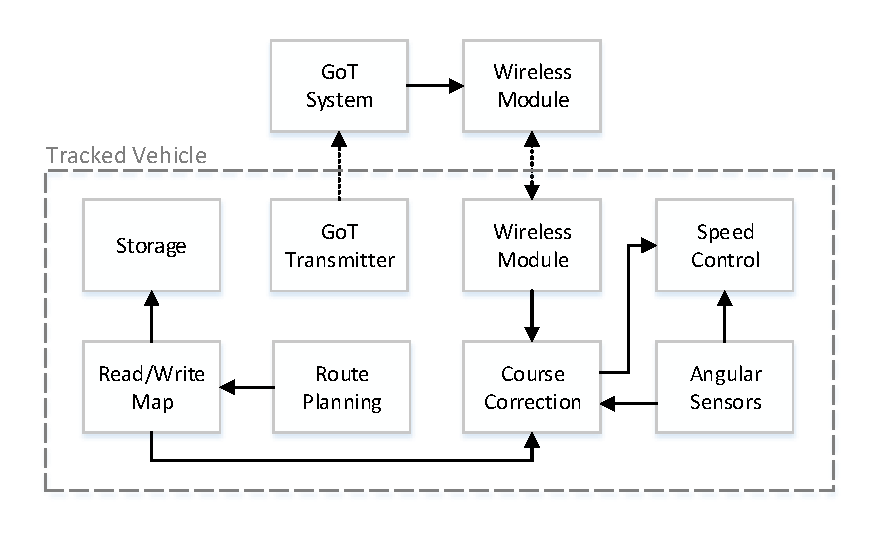
\includegraphics[scale=.9]{figures/systemOverview1}
%	\caption{Overview of the system prototype}
%	\label{fig:systemOverview1}
%\end{figure}

%The GoT system provides the vehicle with coordinates, which is utilized in course correction in combination with the map supplied from storage, to follow the route. In course correction lies also control between coordinates given by the GoT system and the storage, this is regulated through use of angular position and movement supplied by the angular sensors. The speed control gets an input from the course correction, the speed given is then held through regulation again using input from angular sensors, in this case specifically acceleration.


%Previously the rough prototype design is presented. To provide a more broad overview of the system, an exploded view of functionalities, their submodules and interfaces is presented in \figref{fig:systemOverview2}.

The overall functionalities for the project have been constrained from the Use-Case \secref{sec:UseCase}, due to time limitations and to focus on the main scope of the semester. A prototype is therefore made to illustrate the main functionalities necessary to make an automated vehicle, containing principles for lawn mowing.

The final prototype includes a regulator, which will make it possible to follow a path from A to B. It is able to continue if the wireless connection is lost between the prototype and the GoT system for some duration. The outline of the design is shown in \figref{fig:systemOverview2} to give an idea of the final prototype setup. In this section, the different functional blocks are put forth along with the interfaces describing the interaction between them.

\begin{figure}[H]
	\centering
	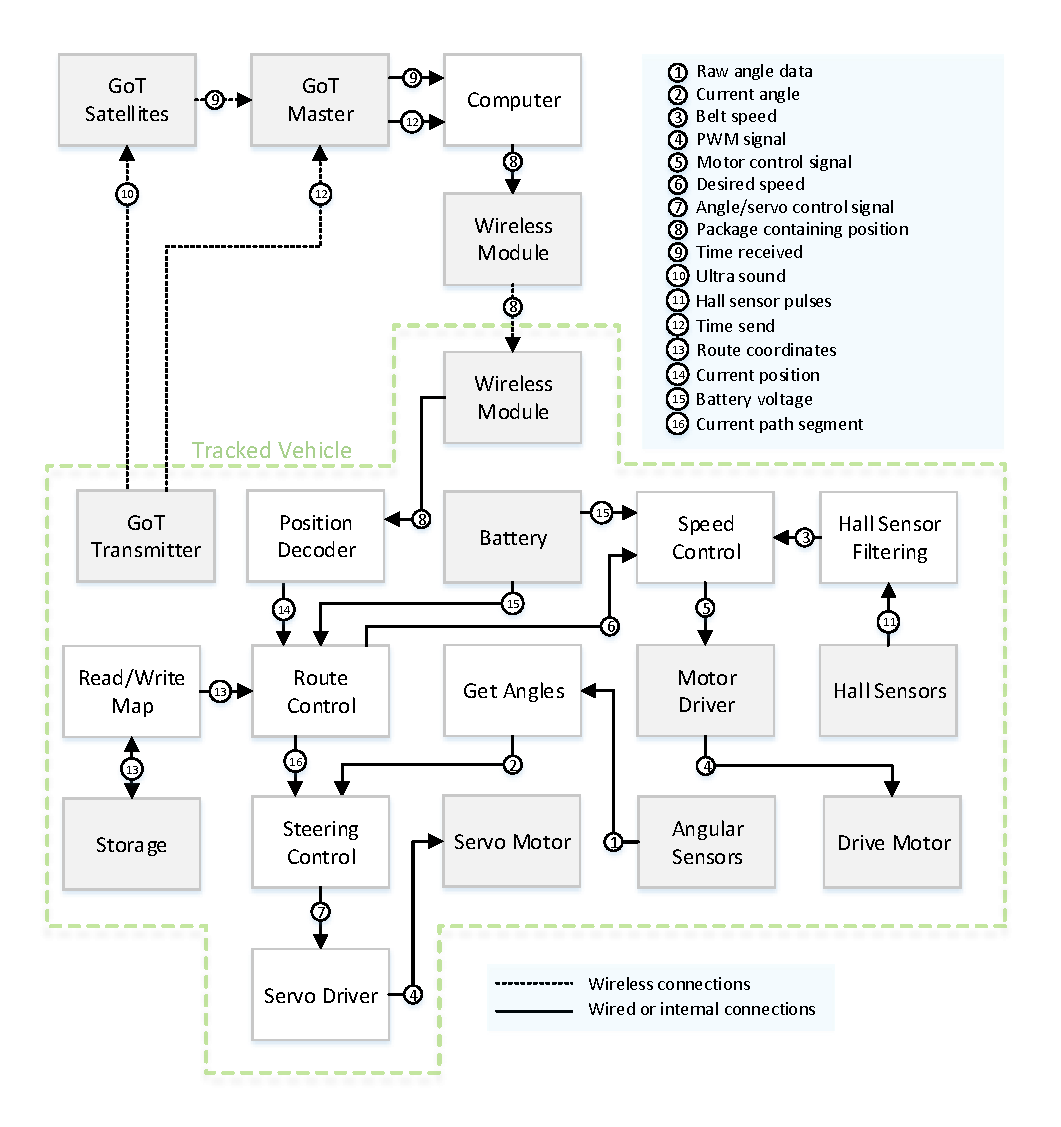
\includegraphics[scale=.9]{figures/systemOverview2}
	\caption{Overview of the software and electronic parts of the system prototype, where the gray modules are hardware and the white are software.}
	\label{fig:systemOverview2}
\end{figure}

\subsection{Modules}
In the following all the modules from the system prototype which needs further explanation are described to obtain a basic understanding of the prototype.

%\subsubsection{GoT System}
%%The GoT satellites is placed in the area in which the vehicle needs to operate. These satellites receives information from the vehicle. The time which the vehicles transmitter sends out bursts is received by the GoT master. Furthermore the time which the satellites receives the information send from the vehicles transmitter is transmitted to the GoT master. The GoT master then relays the information received from the vehicle directly to the 
%
%The \textit{GoT Transmitter} placed on the vehicle transmits a signal containing the time at which it send the ultra sound signal to the \textit{GoT Satellites} to the \textit{GoT Master}. The satellites transmit the signal recieved to the master as soon as they recieve it. The master then relays those informations to the \textit{GoT on Computer} that will calculate the position of the car.

\textbf{Computer and Position Decoder:}
The computer handles the calculation of the current position of the vehicle \secref{sec:Vehicledescription}. If a packet is disturbed or sent incorrectly it should be possible to detect it, so invalid data is not used by the prototype. It may occur that the coordinates which are sent from the GoT system is out of sensible range, e.g the coordinate transmitted jumps from one location to a location which is unrealistic for the vehicle to reach in the amount of time between received coordinates. In this event the out of range coordinate should also be disregarded. The computer must compile a package containing the coordinates. The position decoder must be able to decode the transmitted package.

%\textbf{Route Planning:}
%This module receives the vehicle's position from the GoT and the next destination on the path, which is located in the storage. This information constitutes a desired path segment on which the vehicle must stay. The desired path segment is passed along to steering control.
%The route planning also monitors the battery voltage, and plans a route back to base when the battery starts running low. This is of course to ensure that the vehicle does not get stuck on the lawn, but also to protect the battery, which might get damaged from excessive discharge.

\textbf{Steering Control:}
This module makes sure that the vehicle stays on its path, which it receives from storage. To achieve this the steering control also receives the current path segment of the vehicle, which it uses to calculate a desired angle. The desired angle is used in comparison with the current angle in the steering control to regulate course of the vehicle.

\textbf{Read/Write Map:}
This module handles the writing of coordinates to the non-volatile storage device, as well as the reading of next desired destination from the stored route.

\textbf{Speed Control:}
This module retrieves the speed of the vehicle from the Hall Sensor Filtering module. This is used, through control, to obtain a steady speed. Furthermore it handles any request of change in speed delivered by the course correction.

%\subsubsection{Edge Map}
%The first time the user will initialise the lawn mower, an \textit{Edge Map} will be created thanks to the GoT system. This edge map will determine the areas that the car is allowed to go or not, in regards of specifications or objects on the lawn.  

%\subsubsection{Route Planning}
%The Route Planning module calculates a route from the points gathered from the Edge Map. The route will be in straight lanes, as in the Bosch Logicut system \secref{roboMowers}, to guarantee that the whole lawn is cut.

%\subsubsection{Angular Sensors}
%The angular position is measured thanks to the \textit{Angular Sensors}, that will send data to the submodule \textit{Get Angle}, in charge to send the angle to the Speed Control and to the Course Correction submodule.

\subsection{Interfaces}
%- To Tom and Rasmus \newline
%In the subsection an explanation of the different interfaces between the modules is made. We have thought about making it like a high layer interface, where we only explain what we need the different modules to give each other. Like one module needs to get the map edge, i.e. coordinates, but since it is this early in the report and it would be more overview by writing map edge rather than coordinates. But as you can see in \figref{fig:systemOverview2} the layers of information are different, one is raw angle data and another time send. Is this okay or should we change something else?
%\indent
%The interfaces of the system is very important when designing each of the adjacent submodules. The existing interfaces as well as the ones presumed are also important in the process of analyzing the system capabilities width focus on requirements of the prototype. Width that in mind follows a brief review of the interfaces between each submodule.
In this section a high layer interface between the modules will be presented. This provides information for designing each of the adjacent submodules individually.

\textbf{Package Containing Position (8):}
The data communicated from the GoT system to the Position Decoder on the vehicle contains the last recorded position of the vehicle. This position is presented in the form of an x- and a y-coordinate, which must be included in the data package. Additionally each package must contain decode information for the receiver, including how to separate each package along with error handling.

\textbf{Angle/Servo Control Signal (7) and PWM Signal (4):}
Course correction will ask the vehicle to turn or make small adjustments to the angle. This angle adjustment is realized through the servomotor which brakes on either belt appropriate to the required angle. For the servo to understand the angle, the servo driver must translate it into a PWM signal, which makes the servo turn to a specific position for each pulse width.

\textbf{Route Coordinates (13), Current Position(14) and Battery Voltage (15):}
Route coordinates are extracted from the storage and paired with the current position given by the GoT system. This coordinate pair yields a path segment for the vehicle to follow, which is forwarded to steering control.

\textbf{Raw Angle Data (1), Current Angle (2) and Current Path Segment (16):}
The raw angle data is translated to a current angle of the vehicle. Current angle is then used to calculate the desired angle using the path segment given by route planning.

\textbf{Desired Speed (6), Motor Control Signal (5) and PWM Signal (4):}
Desired speed is regulated by the route control because the route planner knows when the vehicle must turn, in which case the speed should be lowered, if desired. The speed controller makes sure that the vehicle stays at this speed, until told otherwise, by regulation of the motor control signal. This signal is then translated, by the motor driver, to a PWM signal for the motor.

\textbf{Hall Sensor Pulses (11) and Belt Speed (3):}
To determine the speed of the vehicle, two Hall sensors are placed by the drive wheels. These generate pulses transmitted through the filter, which translates it into two separate belt speeds averaged as one for speed control.


%Route Planning, Storage and Read/Write Map Interfaces:
%The Edge Map submodule sends the Map edge to Route Planning, that will send a Route to Read/Write Map. The Route to follow will then be transmited to the Course Correction submodule for a path correction, and to the Storage for saving.

%\textbf{Speed Control Interfaces:}
%The Hall Sensors send Hall sensor pulses to the submodule Get Speed, that will process it to transmit the Belt speed to the Speed Control. A PWM signal containing the new wanted speed will then be sent to the Motor Driver, wich will convert it to the final Motor control signal and sent it to the Drive Motor.
%
%\textbf{Angular Sensors Interfaces:}
%The Angular Sensors will send a Raw angle data to the submodule  Get Angles, that will process it and send the Processed angle data to Course Correction.
%
%\textbf{Course Correction Interfaces:}
%The Course Correction submodule receives the Position and Time from the Wireless Module, the Route to follow from Read/Write Map, and the Processed angle data from Get Angles. With all those information, a decision will be sent to the Speed Control through the Desired speed, and to the Servo Motor with an Angle/servo control signal.

Now that the vehicle is described and the prototype defined, requirements for the prototype can be established.


%---------------------------------------------------------------------------------------------------------------------------\\
%REWRITE THIS SCRAMBLED VERSION OF THE ABOVE TWO SUBSECTIONS \todo{rewrite in the above section and delete these subsections}\\
%---------------------------------------------------------------------------------------------------------------------------
%
%\subsubsection{GoT Satellites, Master and GoT Ultra Sound \& Radio Link}
%\indent
%A number of GoT Satellites are placed in the corners of the area in which the vehicle is to operate. These Satellites receive ultra sound signal from the GoT device placed on the vehicle. The time in which each ultrasound signal is received is passed through a wireless connection from the satellites to the GoT master. The GoT master then pairs this information with the time the ultra sound signal was send from the vehicle which it receives via radio link from the GoT device on the vehicle. After collecting the information, the GoT master sends a calculated position and along with a time stamp to the computer handling GoT.
%
%\subsubsection{Wireless Modules}
%\indent
%%The wireless modules serves the purpose of transmitting the calculated coordinates from the GoT system to the vehicle.
%
%\subsubsection{Edge Map, Route Planning, Read/Write Map and Storage}
%\indent
%%The route planning functionality receives the hard coded edge positions from edge map. Using this information the route is then planned and saved in the storage through the read/write map functionality.
%
%\subsubsection{Gyro, Accelerometer, Magnetometer, Speed Control and Course Correction}
%\indent
%%Gyro along with magnetometer is used for angular position of the vehicle. This is passed to the course correction through the get angle functionality. Here it is used as to correct the orientation of the vehicle on its path. The accelerometer also channels through the get angle functionality. The angular acceleration is then used for correction of the speed.
%
%\subsubsection{Hall Sensor}
%\indent
%%The speed control also receives input from the hall sensors through the get speed functionality, where the inputs from the hall sensors are translated to speed of the vehicle's belts. This information is then used in speed control to regulate the speed.
%
%\subsubsection{Servo Motor}
%\indent
%%The servo motor receives an angle/servo control signal from course correction. This angle equals a given amount of breaking on either of the two belts, which then through the differential gearing translate into steering and thus correction of the course of the vehicle.
%
%\subsubsection{Motor Driver and Drive Motor}
%\indent
%%The drive motor takes a motor control signal from the motor driver provided by the speed control. The control signal from speed control is a PWM signal.            %---- Prototype

%---------- Chapter 3 ---------------------------------------- Requirements
\chapter{Prototype Requirements} \label{Requirements}

\begin{enumerate}
%\item \textbf{It shall be possible to track the vehicle's position}
%	\begin{itemize}
%	\item[] why and from where?
%	\end{itemize}
\item \textbf{It shall be possible for the vehicle to receive it own location wirelessly from the GoT system, through a computer.}
	\begin{itemize}
	\item[] The vehicle needs to be able to receive its own location, additionally, it should be wireless so the vehicle can drive without cables attached, and thereby be able to move freely, \secref{Finalprototype}
	\end{itemize}
\item \textbf{It shall be possible for the prototype to disregard incorrect packets transmitted from the computer}
	\begin{itemize}
	\item[] To ensure that invalid data is not utilized, \secref{Finalprototype}
	\end{itemize}
	\item \textbf{The prototype must be able to disregard erroneous coordinates sent from the GoT system}
	\begin{itemize}
	\item[] If the GoT system delivers an unrealistic coordinate, e.g. created by noise, to the vehicle, \secref{Finalprototype}.
	\end{itemize}
\item \textbf{The prototype must be able to access the route, which it has to follow, from a storage space located on the vehicle}
	\begin{itemize}
	\item[] To simulate the use-case, see \secref{sec:UseCase}, the route needs to be stored on the vehicle, and thereby making it accessible for the functionality course correction, \secref{Finalprototype}.
	\end{itemize}
\item \textbf{The prototype must be able to shut down, if the battery voltage is below its cut-off specification}
	\begin{itemize}
	\item[] To ensure the battery is not damaged, \secref{Finalprototype}.
	\end{itemize}
\item \textbf{It shall be possible for the prototype to follow a predetermined route}
	\begin{itemize}
	\item[] This is to simulate a lawn mower, which is able to cut grass by following a route, \secref{sec:PrototypeConstraints}
	\end{itemize}
\item \textbf{It shall be possible for the prototype to return to the predetermined route if disturbed}
	\begin{itemize}
	\item[] E.g. if the vehicle slips or is moved, \secref{sec:UseCase}
	\end{itemize}
\item \textbf{The prototype shall be able to keep a predetermined velocity when going up - or downhill and when turning}
	\begin{itemize}
	\item[] To ensure an evenly cut of the grass, \secref{sec:UseCase}
	\end{itemize}
\end{enumerate}


%%% Part 2 %%%
\part{Design \& Implementation}
%---------- Chapter 4 ---------------------------------------- Hardware considerations
%% TODO : Move files to appropriate folders when nobody is working on it
\chapter{Hardware and Software\\ Considerations}
From the established requirements for the prototype, it is possible to choose which hardware and software should be utilized. Furthermore, the overall design and implementation of the hardware and software are described.
\section{Hardware Choice} \label{Hardwarechoice}
From the prototype description, see \secref{Finalprototype} it is possible to choose compatible hardware for building the prototype. 
Some of the hardware components are given with the vehicle, see \secref{sec:Vehicledescription}, and therefore, are not described in this section. 
The availability of the components and their compatibility with the system also have to be considered.

%%%%%%%%%%%%%%%%%%%%%%%%%%%%%%%%%%%%%%%%%%%%%%%%%%%%%

\subsection{Microcontroller}
The microcontroller is utilized to control the system and the connected hardware. Thus containing software used for controlling the system by sending and receiving electrical signals as needed.

Requirements for the microcontroller:
\begin{itemize}
% \item Having a CPU, that has a frequency greater than \si{XX\ MHz}. \todo{Number}
\item Having I/O connections, both digital and analogue, see \secref{sec:Vehicledescription}.
\item Having output connections, that can transmit PWM signals, see \secref{sec:Vehicledescription}.
\item Having 5 free timers. Two for the Hall sensors and one for the kernel, motor, servo-motor.
%\item Being powered by an external power source, thereby being able to .
\end{itemize}

\subsubsection{Arduino Mega 2560}
The Arduino Mega 2560 is a microcontroller board, which comes with an 8-bit ATmega2560 integrated circuit and extends its I/O ports, see \figref{ArduinoMega} \cite{MegaInfo}. 

\begin{figure}[H]
	\centering
	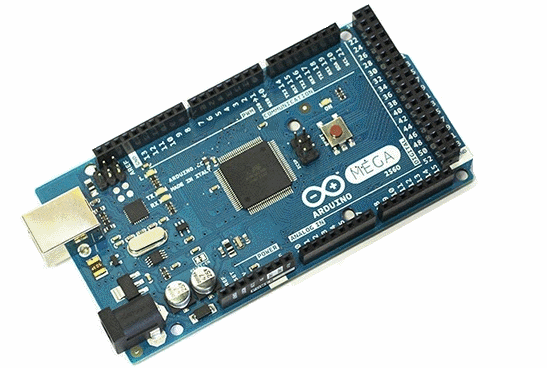
\includegraphics[width=0.5\textwidth]{figures/ArduinoMega.png}
		\caption{An Arduino Mega 2560 board \cite{MegaInfo}} 
	\label{ArduinoMega}
\end{figure}
%
The Arduino Mega has \si{54} digital ports with a 5 volts logic. From these, \si{15} can be used to generate PWM signals. The CPU runs at \si{16 MHz} and the chip has \si{6} integrated timers, one of which is used by the Arduino itself. There are also 4 UARTs, used in serial communication, as well as a setup for SPI communication and an \si{I^2C} bus. The Arduino can be powered though a USB cable or with an external power source.

The Arduino Mega board has been chosen as the microcontroller utilized. The reason is that the connections needed are available. Furthermore, it is possible to find a lot of helpful documentation on the Arduino Mega on the internet. The Arduino is programmable through a serial connection, with the help of avrdude\cite{Avrdude} or simply through the Arduino IDE\cite{ArduinoIDE}. The IDE can compile C, C++ and Arduino (syntax very close to C and C++) files.

%%%%%%%%%%%%%%%%%%%-STORAGE-%%%%%%%%%%%%%%%%%%%%%%

\subsection{Storage}
The storage is used for saving the edge map and the predetermined route for the vehicle see \secref{Finalprototype}.

Prede

Requirements for the storage:
\begin{itemize}
\item Offering the possibility to retrieve the data after a power cut to the storage.
\item Having a storage of \si{XX\ MB}. \todo{Number}
\item Having a transfer speed greater than \si{120\ B/s}. \todo{ref}
\end{itemize}

\subsubsection{SD Card} \label{SDcard}
Secure Digital (SD) card is a type of non-volatile flash memory cards. This means that the data will not be lost during a power cut off.

It comes in various storage sizes, from 1 GB to 2 TB, depending on which type of SD card it is. There is 3 types of SD card, the standard capacity (SDSC), the high capacity (SDHC) and the extended capacity (SDXC). The difference between the different types, is the file system utilized on the card and their maximum capacity. With the requirement of a storage size on XX bytes, and a desired need for utilizing it the contain test data, the SDSC with a capacity of 2 GB is chosen.

The lowest transfer speed for an SDSC card is \si{2 MB/s}. With the requirement of a transfer speed greater than \si{120\ B/s}, makes the SDSC card fast enough. 

To use the SDSC card and connect it to the microcontroller, 7 connection pins are required, see \figref{SDcardpinout}. The setup of the SD card is different, depended on which mode is used.

\begin{minipage}{\linewidth}
      \centering
      \begin{minipage}{0.65\linewidth}
			\begin{table} [H]
				\begin{tabular}{|l|l|l|l|}
								
\hline
\textbf{Pin} & \textbf{SPI}  		& \textbf{One bit} 	& 	\textbf{Four bit}  \\
\hline
1			 &	Unused		 		&	Unused			    &	Data 2			   \\
\hline
2			 &	Card Select	 		&	Card Detection		&	Data 3			   \\
\hline
3			 &	Data In		 		&	\begin{tabular}{@{}l@{}} Command \&  \\Response \end{tabular}  &	\begin{tabular}{@{}l@{}} Command \&  \\Response \end{tabular} \\
\hline
4			 &	Power 				&	Power			    &	Power			   \\
\hline
5			 &	Serial clock 		&	Serial clock		&	Serial clock	   \\
\hline
6			 &	Ground		 		&	Ground			    &	Ground			   \\
\hline
7			 &	Data Out	 		&	Data 0			    &	Data 0			   \\
\hline
8			 &	Unused		 		&	Unused			    &	Data 1			   \\
\hline		
				\end{tabular}
				\caption{SD card pinout configuration}							
			\end{table}			
      \end{minipage}
      \hspace{0.03\linewidth}
      \begin{minipage}{0.30\linewidth}
          \begin{figure}[H]
              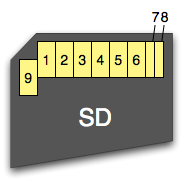
\includegraphics[width=0.95\textwidth]{figures/sdcardpinout}
              \caption{Illustration of a micro size SD card.} % http://elasticsheep.com/2010/01/reading-an-sd-card-with-an-atmega168/
              \label{SDcardpinout}
          \end{figure}
      \end{minipage}
      
  \end{minipage}

The power needed for the SD card is 3.3 volts. There are three possible setups for the SD card: SPI, One-Bit and Four-Bit.
With the SPI setup, the communication between the SD card and the microcontroller is made on two lines. With the One-Bit setup, the commands between the SD card and microcontroller are sent on one line and the data is sent through another one.
With the Four-Bit setup, three more data connections are used.

In this project, the SPI setup is used, since the extra transfer speed from the Four-Bit setup is not needed. Furthermore, the Arduino has 4 pins that can be set up to SPI communication.

An SDSC card, with a SPI setup is chosen, since this as has a high enough capacity and transfer speed, and therefore meets the requirements. Furthermore the data is saved, if the power is cut off and the Arduino Mega has SPI connections. 

%%%%%%%%%%%%%%%-Motor Driver-%%%%%%%%%%%%%%%%%%%%

\subsection{Motor Driver}
The motor driver is the connection between the microcontroller, the power supply and the motor. It is used, to isolate the hardware components functioning in low power, i.e. the microcontroller, from the high power parts, i.e. the motor.

The requirements for the motor driver are:
\begin{itemize}
\item Having to be controlled by the microcontroller.
\item Offering the possibility to power it through an external power source.
\item Being able to handle the battery pack's voltage.
\item Allowing to power the motor in both directions.
\end{itemize}

\subsubsection{Pololu Dual VNH5019}
The Pololu dual VHN5019 motor driver shield (see \figref{MotorDrive}) is specially designed for Arduino boards. It can be placed directly on top of the the Arduino board as a shield, with the pins connecting to the right ports on the Arduino.\cite{PCorporation}

\begin{figure}[H]
	\centering
	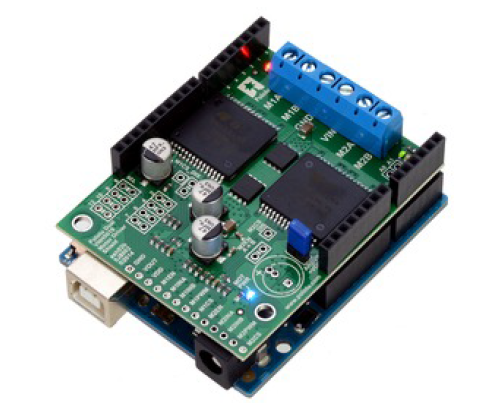
\includegraphics[width=0.50\textwidth]{figures/Motordriver.png}
		\caption{The motor shield on top of an Arduino Uno.} 
	\label{MotorDrive}
\end{figure}

It is possible to power the Arduino from an external power source through the motor shield, which also delivers the power to the motor. It is also possible to have the motor shield and the Arduino powered separately. This is determined by a jumper setting on the shield, see \figref{MotorDriveIO}. The motor shield need a power voltage between 7 volts and 12 volts.\cite{PCorporation}

\begin{figure}[H]
	\centering
	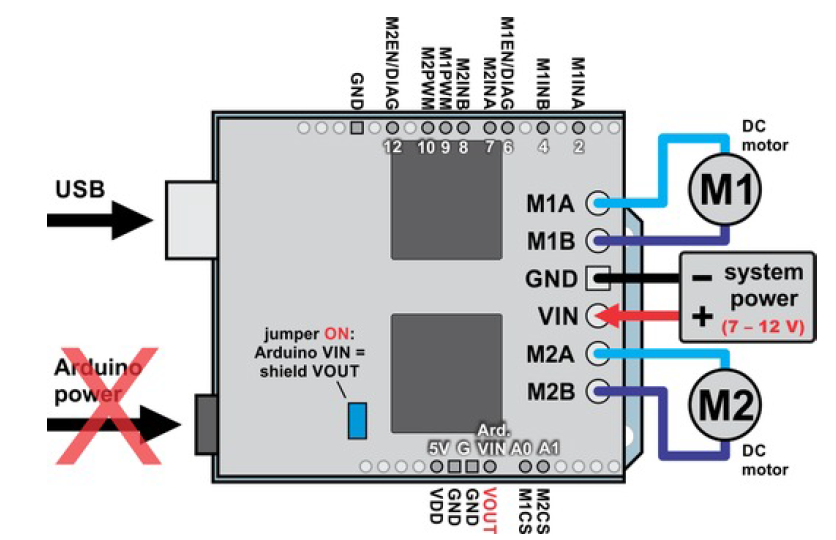
\includegraphics[width=0.60\textwidth]{figures/MotordriverIO.png}
		\caption{Setup for the mort shield.}
	\label{MotorDriveIO}
\end{figure}

There are two H-bridges on the board, to control up to two motors. Since only one motor is used in this project, both of the two H-bridges will be used to power the motor, see further details on the configuration in \secref{sec:HBridge}. This results in a smaller current through the two H-bridges' transistors and therefore ensures a better protection of the system.\cite{PCorporation}

%\begin{figure}[H]
%	\centering
%	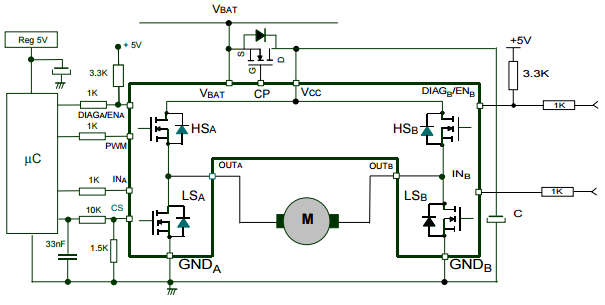
\includegraphics[width=0.85\textwidth]{figures/Hbridges.png}
%		\caption{Illustration of the H-bridge, that the motor shield have two of.}
%	\label{Hbridges}
%\end{figure}
%
The Pololu dual VHN5019 motor driver shield is used in this project, as it is made for the Arduino and therefore easy to implement. Moreover, it can power the Arduino through an external power source and get a power output high enough for the motor and in each direction.\cite{STMicroelectronics}
%%%%%%%%%%%%%%%%%%%%%%%%%%%%%%%%%%%%%%%%%%%%%%%%%%%%%

\subsection{Wireless communication system}
The data from the GoT system is sent to the microcontroller with this comunication system. The transmitter will be located on the computer used for the GoT system and the receiver on the vehicle. As the prototype will be tested in the control lab, the distance that the wireless communication have to send is less than 10 meters.

The requirements for the wireless communication components are:
\begin{itemize}
\item Having to be controlled by the microcontroller.
\item Having a range greater than 10 meters. 
\item Offering the possibility to be powered by an external power supply (through the Arduino power lines).
\item Transfering at a higher rate than \si{120\ B/s}. \todo{ref}
\item Offering the possibility to control it and couple it with the GoT code.
\end{itemize}

\subsubsection{Xbee}\label{Xbee}
Xbees are small radio modules, that are easy to set up. An overview of the Xbee and its pin layout can be seen on \figref{XbeeLook} and \figref{Xbeepinout}.


\begin{minipage}{\linewidth}
	\centering
	\begin{minipage}{0.45\linewidth}      
		\begin{figure}[H]
			\centering
			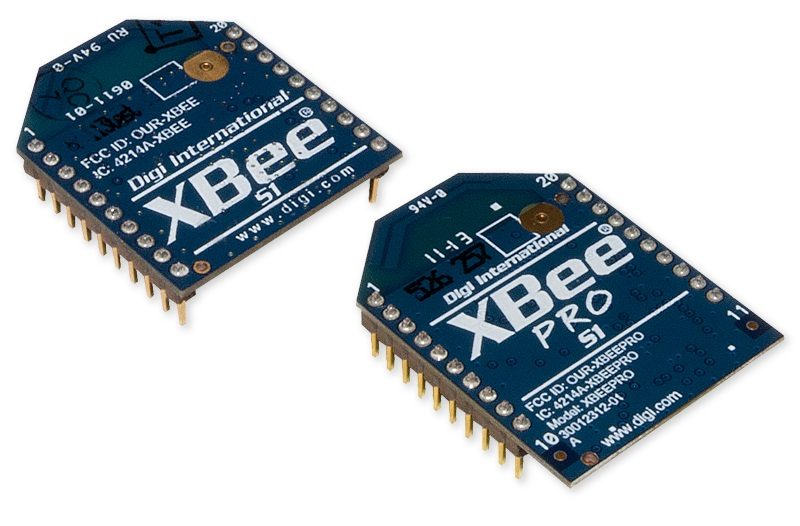
\includegraphics[width=0.95\textwidth]{figures/Xbee.jpg}
			\caption{Two Xbee radio modules} 
			\label{XbeeLook}
		\end{figure}
	\end{minipage}
	\hspace{0.03\linewidth}
	\begin{minipage}{0.45\linewidth}
		\begin{figure}[H]
			\centering
			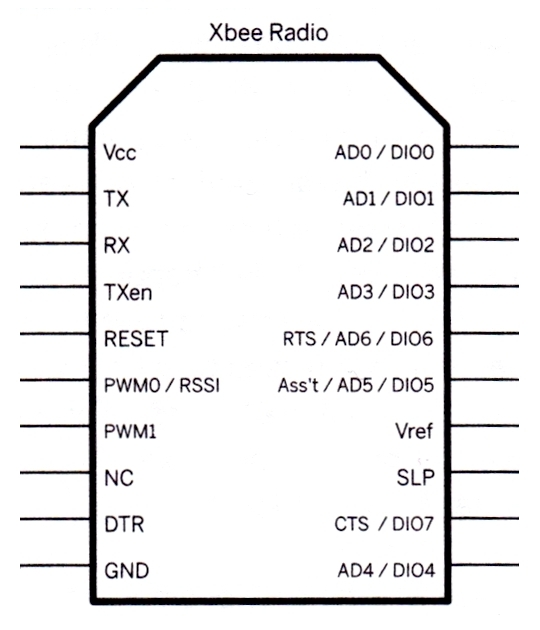
\includegraphics[width=0.95\textwidth]{figures/XbeeIO.jpg}
			\caption{Pinout of an Xbee radio module} 
			\label{Xbeepinout}
		\end{figure}
	\end{minipage}
\end{minipage}

\todo{Snak med vinkel om at få teksten align}

The Xbee modules communicate through an UART connection (with TX and RX pins). Since the Arduino has three UART connections plus the one used to program the Arduino, the Xbee can be connected. The software code for the GoT system is implemented in C\# (see in \secref{GoTDescription}) and the computer running has serial ports that can ensure the connection between the software and the Xbee. Therefore, this solution can be used for a wireless connection between the GoT system and the Arduino.

To run the Xbee modules, a \si{3,3\ V} power line, a ground line, and a \si{3,3\ V} logic UART are needed. The rest of the pins are not needed in this project. The modules have a transfer speed of up to \si{115,2 kbit/s} and can reach up to \si{100 m} indoor and \si{300 m} outdoor. It transmits at a \si{2,4 GHz} frequency with \si{1 mV} (\si{0 dBm}) and can receive downto \si{-96 dBm}. The Xbee is already ready for communication, with the lower levels of communication, the physical and data link layers, being already implemented. With only two devices, a lightweight combination of transport and presentation layer can be added to the protocol directly on top of the data link layer, to add more error handling and to set up how the data shall be sent.

%http://www.digi.com/products/xbee-rf-solutions/modules/xbee-digimesh-2-4#specifications

%%%%%%%%%%%%%%%%%%%%%%%%%%%%%%%%%%%%%%%%%%%%%%%%%%%%%

\subsection{Angular sensor}
The angular sensor is used in the feedback for the control system.

The requirements for the angular sensor are:
\begin{itemize}
\item To be controlled by the microcontroller.
\item Having a sampling frequency greater than XX. \todo{Number}
\item Having a latency smaller than XX. \todo{Number}
\item Offering the possibility to power it by an external power supply (through the Arduino power lines).
\end{itemize}

\subsubsection{HMC5883L}
Sparkfun's "9 degrees of freedom" board comprises a magnetometer integrated circuit, the HMC5883L\cite{HMC5883L}. A magnetometer will be used as the angular sensor, since it can be set up as a compass and give out a angle compared to north. As the direction to north is always the same, the system does not need a new calibration of the angular sensor, if used in a new area. However, it has to be calibrated on the vehicle when used for the first time.

\begin{figure}[H]
	\centering
	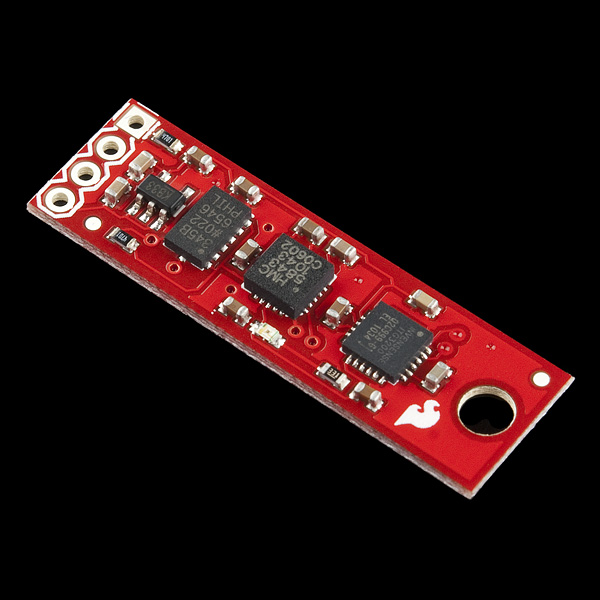
\includegraphics[width=0.50\textwidth]{figures/NineDegree.jpg}
		\caption{Sparksfun's "9 degrees of freedom" sensor stick} 
	\label{NineDegree}
\end{figure}

The "9 degrees of freedom" sensor stick, see \figref{NineDegree}, will be used in the project. Beside the magnetometer, there are also a accelerometer and a gyroscope on the board, but these will not be used. The "9 degrees of freedom" sensor stick is designed to be used with a microcontroller and comes with software example for the Arduino platform. It needs an  \si{I^2C} bus to communicate with the Arduino, which has that kind of interface.

%%%%%%%%%%%%%%%%%%%%%%%%%%%%%%%%%%%%%%%%%%%%%%%%%%%%%

\subsection{Power monitor}
The power monitor is used to give a feedback to the system about the level of power in the battery pack.

The requirements for the angular sensor are:
\begin{itemize}
\item Being monitored by the microcontroller.
\item Measuring the battery pack voltage output downto \si{5,7\ V}.\todo{ref}
\end{itemize}

\subsubsection{Voltage divider}
A voltage divider is an electronic circuit, that divides the input voltage with a constant depending on the values of the resistors used in the circuit, see \figref{VoltDivFig}.

\begin{figure}[h!]
\centering
\begin{circuitikz}
\draw (0,0)
to[V,v=$V_{in}$] (0,2)
to[short] (2,2)
to[R=$R_1$] (2,0)
to[R=$R_2$] (2,-2)
to[short] (0,-2)
to[short] (0,0);
\draw (2,-2) 
to[short] node[ground] {} (2,-3);
\draw (2,0)
to[short] (3,0)
to[short,l=$V_{out}$] (4,0);
\end{circuitikz}
\caption{Standard voltage divider} 
\label{VoltDivFig}
\end{figure}

The output of the voltage divider can be find with \eqref{VoltageDivider}. 

\begin{flalign}
\eq{V_{out}}{\frac{R_2}{R_1 + R_2} \cdot V_{in}}\unit{V} 
\label{VoltageDivider}
\end{flalign}
\hspace{6mm} Where:\\
\begin{tabular}{p{1cm}lll}
& \si{V_{in}} & is the battery pack voltage &\unitWh{V} \\
& \si{R_1, R_2} & are two calculated resistors &\unitWh{\Omega}\\
& \si{V_{out}} & is the measured output voltage &\unitWh{V}
\end{tabular}

The input voltage is set to be the battery pack and the output is measured though an analogue pin on the Arduino. The analogue pin on the Arduino can measure from \si{0\ V} to \si{5\ V} with a resolution of \si{10\ bits}. This gives 1023 steps from 0 to 5 volts and each step is \si{4,9\ mV}. The size of each step and the range for the measuring is multiplied with the inverse constant, that comes from the two resistor, so it is possible to make the range go over \si{5\ V}. 

A voltage divider is used in this project, as it can be scaled to the interval that it has to measure. The voltage divider will be connected to an analogue pin on the Arduino, which will make the measurement from the output of the voltage divider.\\

From the requirements for the system to the hardware parts, these components have been chosen. After having chosen the different hardware components for the prototype, the different components have to be implemented in the system.
%%%%%%%%%%%%%%%%%%%%%%%%%%%%%%%%%%%%%%%%%%%%%%%%%%%%%


%Pins on the arduino
%SD card (4 I/O)
%Xbee (1 TX and 1 RX)
%Hall (2 I/O)
%Angular (1 SDL and 1 SDA)
%Servo (1 PWM)
%Motor (1 PWM)

\section{Hardware Implementation}
With the hardware components being chosen, it is necessary to assemble them, ensure that they are compatible for communication with the microcontroller, and that they receive the appropriate electrical power. Other implementation considerations also have to be considered. e.g , the voltage divider for the power monitor.
\subsection{Microcontroller peripherals}
Before choosing which pins on the Arduino Mega to connect the various hardware to, the peripherals\footnote{Hardware modules, such as timers, UARTs, etc.} in the microcontroller needs to be evaluated (each peripheral is only available on certain pins). First, the timers are considered. The microcontroller has 6 hardware timers, Timer 0 to Timer 5.

Timer 0 is reserved by the Arduino for it's internal time keeping functions, and not to be touched \cite{ArduinoPWM}. This leaves 5 timers, that can be used freely.

It would be advantageous to utilize the input capture\footnote{An input capture timer samples a free running counter, whenever triggered by  an external event} functionality of the timers to read the hall sensors, since it will provide a hardware generated timestamp, and be independent of software latency. After examining the Arduino Mega pinout, \appref{megaPinout}, it is seen that only Timer 4 and 5 have their input capture pins available on the board (ICP4 and ICP5). These are therefore chosen for the two hall sensors.
   
The real-time operating system needs a timer, for running its scheduler. Timer 1 is chosen for this, for no other reason than it being the default setting.

This leaves Timer 2 and 3. According to \cite{Atmega}, Timer 2 is an 8 bit timer, and Timer 3 is 16 bit. 

Timer 3 is chosen for the PWM signal sent to the servo. This, because the higher resolution makes it easier to generate the short duty cycles required by the servo (\si{500\ \mu s} to \si{2500\ \mu s} on-time, in a \si{30\ ms} period, see \subsecref{Servo})

The last timer is chosen for the PWM signal to the DC-motor.

As the timers have now been designated, the next step is to assign the various serial ports. This is done as shown on \figref{MegaSetup}. Considerations about the powering of the hardware modules is seen in \secref{sec:elecConsiderations}.	


\begin{figure}[H]
	\centering
	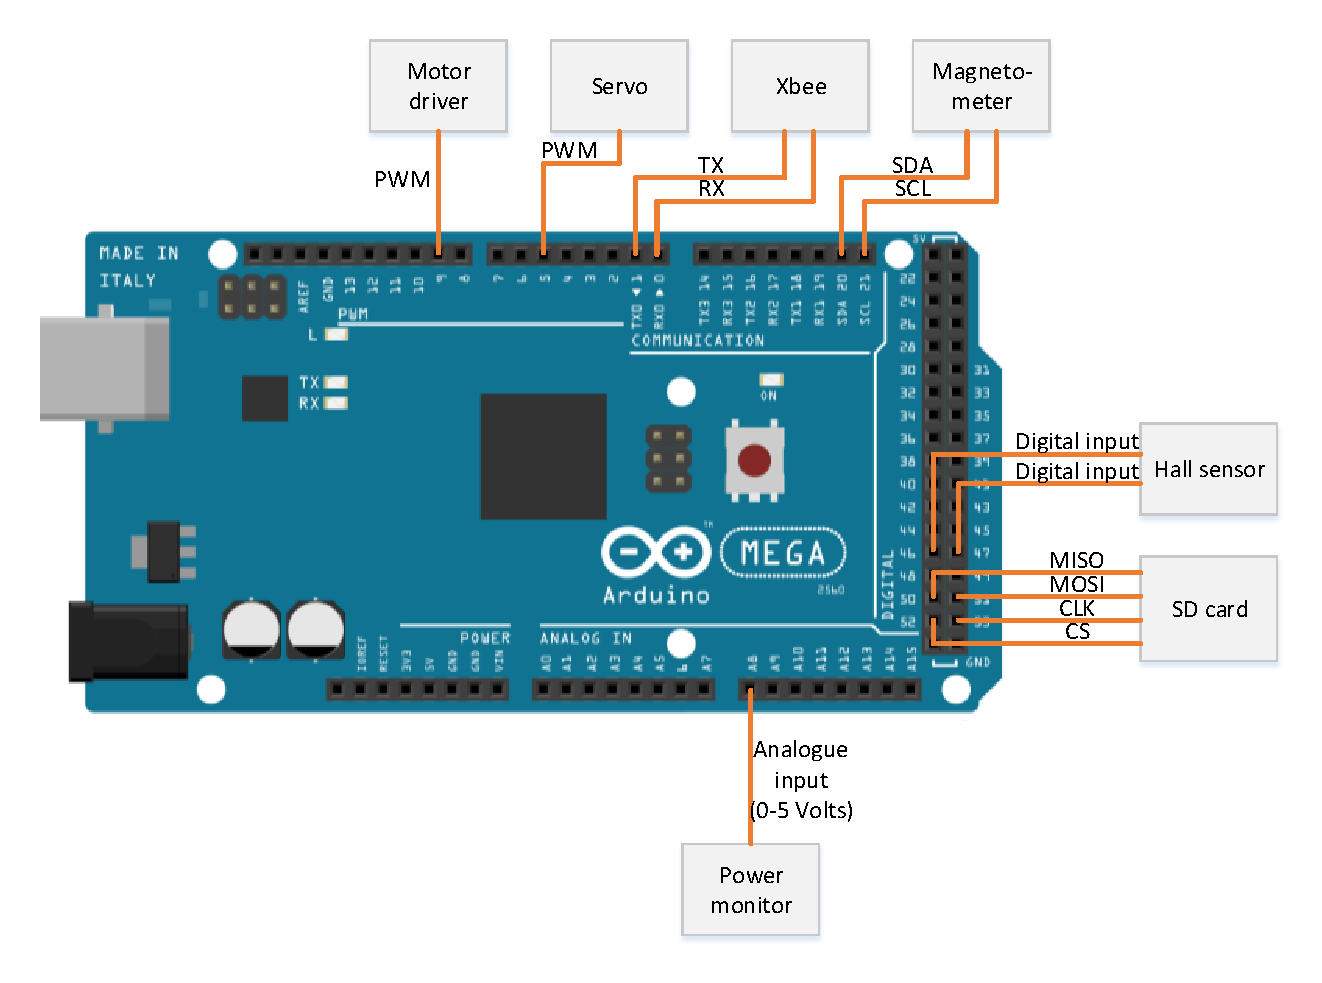
\includegraphics[scale=0.75]{figures/MegaSetup.pdf}
	\caption{Connections between the different hardware components and the Arduino.\cite{ArduMega}}
	\label{MegaSetup}
\end{figure}

The XBee module needs to connect to a serial port, and UART3 is chosen, as it makes it easier to route the PCB traces. UART3 is located at pins 0 and 1. 

The SD card needs an SPI connection, and must therefore be connected to the SPI pins 50, 51, 52 and 53. 

The "9 Degrees of Freedom" board needs an $\text{I}^2\text{C}$ connection, and has to be connected to the Arduino's $\text{I}^2\text{C}$ pins 20 and 21. 

The PWM signals sent to the motor and servo can be set to any of the PWM pins. For easier routing, pin 9 for the motor and pin 5 for the servo is selected.

The input from the hall sensors will be measured by the input capture pins (ICP4 and ICP5), to which Timer 4 and Timer 5 are connected. On the Arduino board, it corresponds to the pins 46 and 47.

Lastly, the voltage divider used for the power monitoring is connected to an analogue pin chosen to be pin A9.

As all hardware modules have now been assigned pins on the Arduino, the electrical requirements of each module will now be considered.

\subsection{Electrical considerations}\label{sec:elecConsiderations}

Before connecting hardware modules to the Arduino pins, signal voltage levels also need to be considered:

\begin{itemize}
\item The Arduino Mega 2560 itself uses 5V logic levels.\cite{MegaInfo}
\item The "9 Degrees of Freedom" board needs \SI{3,3}{V}-\SI{16}{V} supply and $\SI{3,3}{V}$ logic levels. \cite{9dog}
\item The servo needs $\SI{4,8}{V}$ to \si{6\ V} supply voltage and signal levels.\cite{futaba}
\item The SD card needs $\SI{3,3}{V}$ supply voltage and signal levels, see \subsecref{SDcard}.
\item The Hall sensors needs $\SI{3,5}{V}$ to \si{24\ V} supply, and a pull up resistor to define the logic level.
\cite{HallDS}
\item The XBee module needs $\SI{3,3}{V}$ supply voltage and signal levels.
\subsecref{Xbee}
\end{itemize} 

The Arduino has regulated 5V and $\SI{3,3}{V}$ supply rails available, which will be used to power the respectable hardware modules. As the servo can potentially draw a lot of current, and overload the Arduino, it will be connected to a dedicated 5V voltage regulator, powered directly from the battery.

A low-dropout type is chosen, L4941, to make sure it works, even at low battery voltages. This regulator has a maximum dropout of 700mV at 1A current, meaning that it will work with battery voltages as low as $\SI{5,7}{V}$. \cite{L4941} 

All one-directional connections from the Arduino to  $\SI{3,3}{V}$ logic level inputs will be connected to a HEF4050 CMOS buffer. This device can accept input voltages up to 15V, while supplied by as little as 3V supply voltage \cite{4050B}. This makes it ideal for uni-directional voltage level translation. 

One-directional connections from  $\SI{3,3}{V}$ logic level output to Arduino inputs will be connected directly, as $\SI{3,3}{V}$ is above the minimum high level threshold \cite{Atmega}.
%
\begin{flalign}
\eq{V_{IH,min}}{0,6 \cdot V_{cc}}& \nonumber \\
\eq{V_{IH,min}}{0,6 \cdot 5}& \nonumber \\
\eq{V_{IH,min}}{3} \si{\ V}& \nonumber
\end{flalign}

As the $\text{I}^2\text{C}$ bus is using bi-directional connections, and needs to connect a $\SI{3,3}{V}$ system to a 5V system, this needs to be addressed as well. One solution could be running the bus at $\SI{3,3}{V}$, but this is unfortunately not possible, as the microcontroller needs at least $\SI{3,5}{V}$ as HIGH voltage, when in  $\text{I}^2\text{C}$ mode \cite{Atmega}. The creators of $\text{I}^2\text{C}$, Philips, recommend solving this with two MOSFETs \cite{Philips}, see \figref{i2clevel}.

\begin{figure}[H]
	\centering
	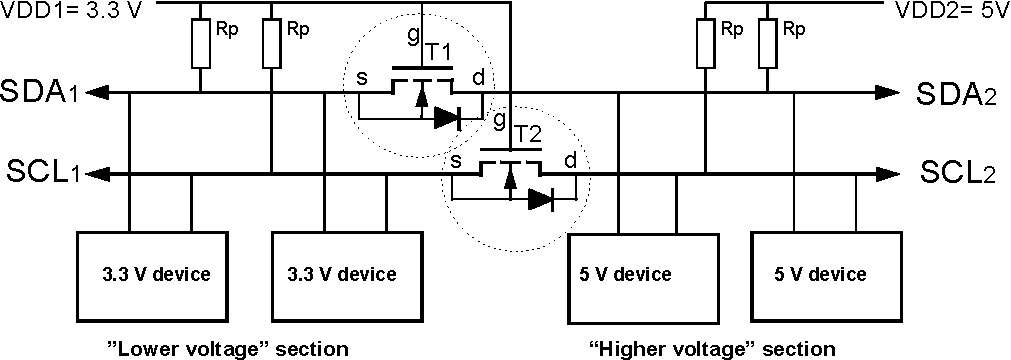
\includegraphics[scale=0.9]{figures/i2cLevel.pdf}
	\caption{$\text{I}^2\text{C}$ Voltage level translator. \cite{Philips}}
	\label{i2clevel}
\end{figure}

In $\text{I}^2\text{C}$ systems, the nodes can only pull the line LOW. To make it possible to signal a HIGH, pull-up resistors are used. If a low voltage system is directly connected to a higher voltage system, the voltage at the input pins of the low-voltage section risk being pulled up to 5V.

To solve this, the translator uses a MOSFET per signal line, with the gate connected to the lower supply voltage, to separate the two systems. Here is a quick explanation, examining just one line (as both lines are implemented identically):\\
%
The gate of the MOSFET is connected to \SI{3,3}{V}.
Four states are possible, both sides HIGH, both sides LOW, or one of each.
If both ends are in the HIGH state, the voltage on the source pin will be \SI{3,3}{V}, and the gate-source voltage will therefore be $\SI{3,3}{V}-\SI{3,3}{V}=\SI{0}{V}$. The MOSFET is therefore off, and not conducting. This prevents the 5V supply from reaching the input of the \SI{3,3}{V} side.\\
If the \SI{3,3}{V} section is in the LOW state, the voltage on the source pin will be 0V, and the gate-source voltage will therefore be $\SI{3,3}{V}-\SI{0}{V}=\SI{3,3}{V}$, turning the MOSFET on. This in turn pulls the 5V section to 0V, signalling a LOW.\\
If the 5V voltage section is in the LOW state, the intrinsic diode in the MOSFET will conduct, pulling the source pin down to \si{0\ V} plus a diode drop ($\approx\SI{0,6}{V}$). This results in a gate-source voltage of $\SI{3,3}{V}-\SI{0,6}{V}=\SI{2,7}{V}$, turning the MOSFET on. This will eliminate the diode drop, and the result will be 0V on the source pin, signalling a LOW to the \SI{3,3}{V} side.

For this to work, a MOSFET that will turn on at \SI{2,7}{V} is needed. FDV303N is available and choosen, as it has a $\text{V}_\text{ds}$ threshold voltage\footnote{The  $\text{V}_\text{ds}$ threshold is the voltage, where the MOSFET starts to conduct} of maximum \SI{1,5}{V}. At \SI{2,7}{V}, the drain-source resistance is specified to \SI{0,6}{\Omega}, meaning that the MOSFET will be on at this voltage\cite{MOSFET}.

\subsection{Voltage divider}

The power monitor need a voltage divider, see \secref{Hardwarechoice}. With a measurement interval of 0 to 5 volts in 1023 steps for the analogue pin on the Arduino, the voltage divider has to be designed to be able measure the whole interval for the battery pack. As the battery pack can have a voltage up to \si{9,0\ V}\cite{BatteryDS}, the transfer constant for the voltage divider need to be smaller than 0,59 to measure the whole interval. The smaller the transfer constant, the bigger the interval is and the bigger each step will be. To make sure that there will not come a bigger voltage than 5 volts on the output from the voltage divider, the transfer constant is set to 0,5: this will give a maximum voltage into the voltage divider of 10 volts before the output voltage goes beyond 5 volts. To get a transfer constant of 0,5, the resistors in the voltage divider have to be the same, see \eqref{VolDivRes3}.\\
%
If,
\begin{flalign}
R &= R_1 = R_2  \unit{\Omega} \nonumber\\
\text{Then,}\nonumber\\
\eq{V_{out}}{\frac{R}{R + R} \cdot V_{in}}\unit{V} \nonumber \\
\eq{V_{out}}{\frac{1}{2} \cdot V_{in}}\unit{V}
\label{VolDivRes3}
\end{flalign}
%
For the size of the resistors, the output impedance for the voltage divider have to be taken into consideration. For the analogue pins on the Arduino, it is recommended to have a output impedance smaller than \si{10\ k\Omega}, or the it will begin to disturb the reading on the pin.\\
To make sure that this does not happen, the resistors in the voltage divider are set to half of the maximum output impedance, \si{5\ k\Omega}. The closest resistor in the E96 series is \si{4,99\ k\Omega}, which will be used for both resistors. 

The final voltage divider circuit for the power monitor can be seen on \figref{VoltDivFigFinal}.
\begin{figure}[h!]
\centering
\begin{circuitikz}
\draw (0,2)
to[short,l=$V_{in}$] (1,2)
to[short] (2,2)
to[R=$R_1$] (2,0)
to[R=$R_2$] (2,-2);
\draw (2,-2) 
to[short] node[ground] {} (2,-3);
\draw (2,0)
to[short] (3,0)
to[short,l=$V_{out}$] (4,0);
\draw (2,0)
to[C=$C_1$] (0,0)
to[short] node[ground] {} (0,-1);
\end{circuitikz}
\caption{The implemented voltage divider} 
\label{VoltDivFigFinal}
\end{figure}

To filter the high frequency noise out, a simple low-pass RC filter is finally implemented with a 1 $\mu$F capacitor in the voltage divider. The resulting cut-off frequency is then:
%
\begin{flalign}
\eq{\omega_{c}}{\frac{1}{R \cdot C}}\unit{rad \cdot s^{-1}} \nonumber \\
\eq{\omega_c}{\frac{1}{2,5 \cdot 10^{3} \cdot 1 \cdot 10^{-6}}}\unit{rad \cdot s^{-1}} \nonumber \\
\eq{\omega_c}{400}\si{\ rad \cdot s^{-1}}&\nonumber
\end{flalign}

With all the hardware components physically implemented on the vehicle and connected to the microcontroller, the software utilized needs to be determined and designed to enable interactions between the Arduino and all the hardware components.
\section{H-Bridge}
The H-bridge see \figref{Hbridge} is a commonly used circuit for motor control. To control the motor some FET(s) are controlled with a PWM signal. The duty cycle of this PWM signal determines at which velocity the motor will run.

\begin{figure}[H]
	\centering
	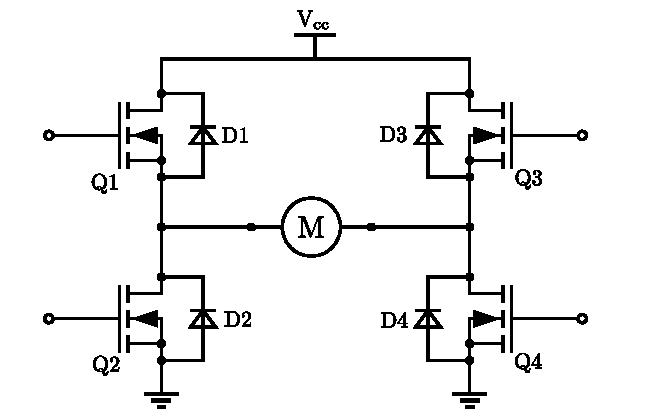
\includegraphics[scale=.6]{figures/Hbridge.pdf}
	\flushleft
	\caption{Standard H-bridge}
	\label{Hbridge}
\end{figure}


There exists a wide range of configurations in which the H-bridge can be implemented. These configurations determines the modes of operation, where each mode has some different properties. Some of the common modes are described in the following sections.

\subsection{Regenerative Coast Mode}

\begin{figure}[H]
	\centering
	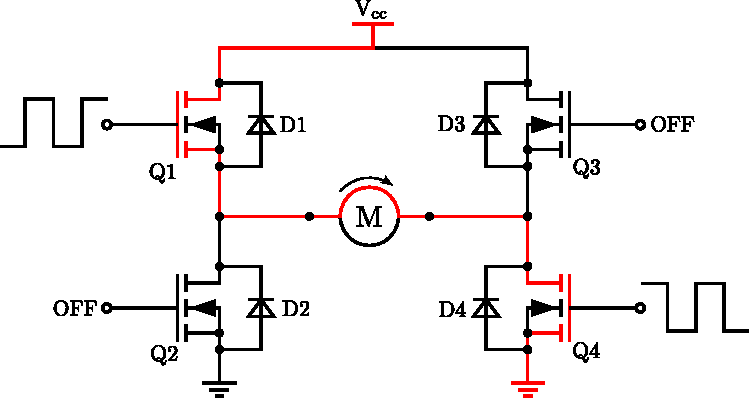
\includegraphics[scale=.6]{figures/HbridgeClockwiseCoastON.pdf}
	\flushleft
	\caption{Clockwise coast operation in on-state}
	\label{figures/HbridgeClokwiseCoastON}
\end{figure}

\begin{figure}[H]
	\centering
	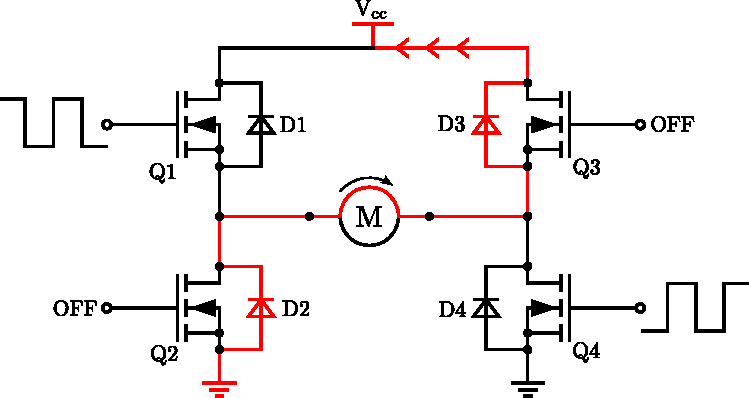
\includegraphics[scale=.6]{figures/HbridgeClockwiseCoastRegen.pdf}
	\flushleft
	\caption{Clockwise coast operation in off-state}
	\label{HbridgeClokwiseCoastRegen}
\end{figure}

\subsection{4Q Mode}

\begin{figure}[H]
	\centering
	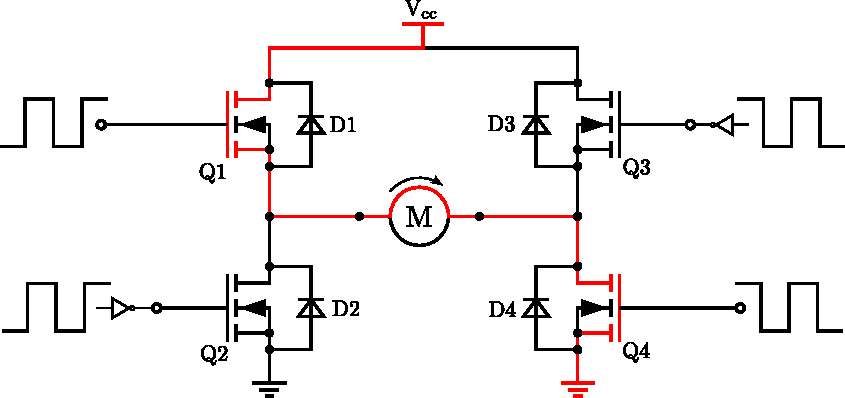
\includegraphics[scale=.6]{figures/HbridgeClockwise4Q.pdf}
	\flushleft
	\caption{Clockwise 4Q operation}
	\label{HbridgeClokwise4Q}
\end{figure}

\begin{figure}[H]
	\centering
	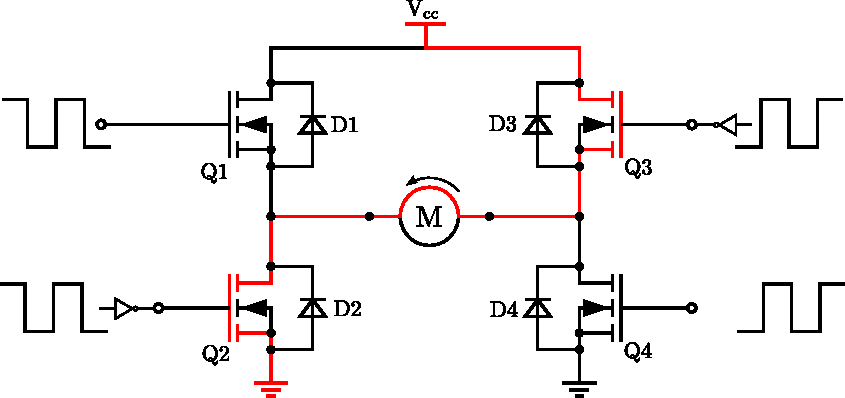
\includegraphics[scale=.6]{figures/HbridgeCounterClockwise4Q.pdf}
	\flushleft
	\caption{Counterclockwise 4Q operation}
	\label{HbridgeCounterClokwise4Q}
\end{figure}

\subsection{Brake Mode}

\begin{figure}[H]
	\centering
	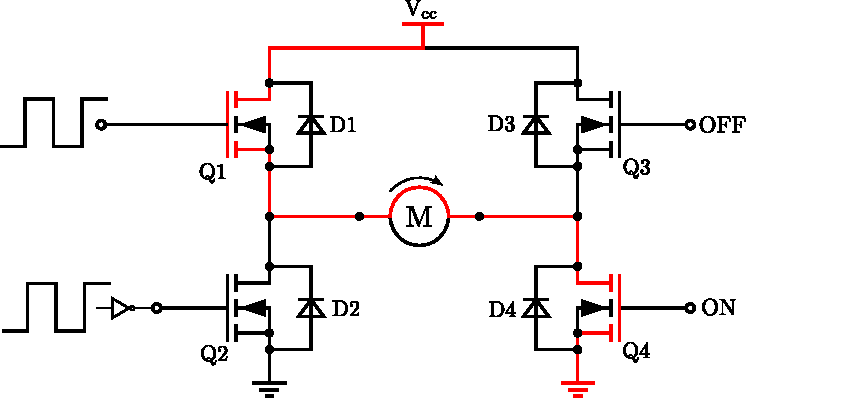
\includegraphics[scale=.6]{figures/HbridgeClockwiseBrakeON.pdf}
	\flushleft
	\caption{Clockwise brake operation in on-state}
	\label{HbridgeClockwiseBrakeON}
\end{figure}

\begin{figure}[H]
	\centering
	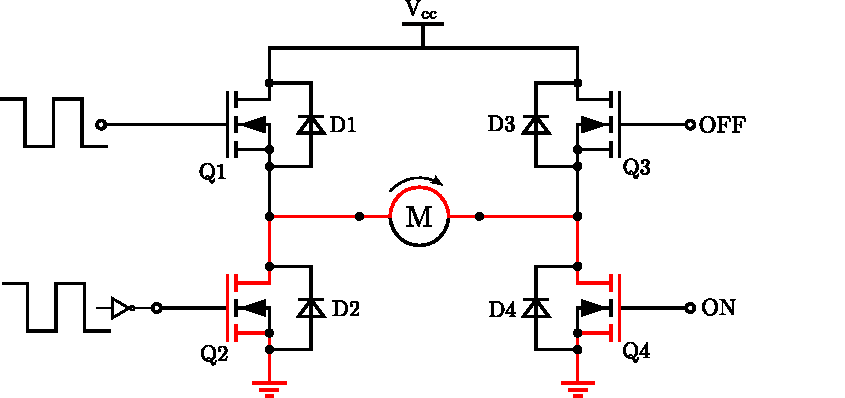
\includegraphics[scale=.6]{figures/HbridgeClockwiseBrakeOFF.pdf}
	\flushleft
	\caption{Clockwise brake operation in off-state}
	\label{HbridgeClockwiseBrakeOFF}
\end{figure}
\section{Software Choice}
For the hardware components to interact, software parts are needed to handle them. The software choice is explained in this section, which describes the use of the chosen RTOS (Real Time Operating System), and the principle of scheduling.

\subsection{Real Time Operating System}
The chosen RTOS is a stable open source project named KRNL, written by the Associate Professor Jens Dalsgaard Nielsen from Aalborg University.\\
Specially written for the Arduino platform, it allows to control the tasks, and therefore the behaviour of the vehicle, through a timer, to keep a precise and constant time schedule. This property makes it possible to export it to another kind of processor and still have the same render, as long as it have a frequency high enough to process all the data needed.\\
One of KRNL's advantage is also the definition of semaphores, priorities, and critical regions, that the system will use to choose which task to run, and how often to run it. Futhermore, this RTOS allows to program in Arduino language, which is a C\texttt{++} extension, and can also run C code, using different files.

\subsection{Scheduling}\label{sec:scheduling}
To run the code on the Arduino microcontroller, and be able to manage all the sensors in parallel and at the time needed, a scheduling scheme is needed. Indeed, the microcontroller must be able to receive and process the data from the GoT computer received through the XBee module, the Hall sensors and the magnetometer. From all this data, it also has to make a decision regarding the planned route to follow. This decision must affect at the same time the speed of the motor, and the steering through the servo.
A description of the scheduling principle and its function will now be described.


\subsubsection{Semaphores}
In programming, a semaphore is a variable or abstract data that is used to prioritize the different tasks to use. It allows a multiprogramming, with functions that use different resources and time, and does not interact with each others directly. Running them independently ease the development of the code.

\newpage
\subsubsection{Tasks}
The different functions of the vehicle have been separated into multiple tasks, that can switch regarding to their priority. Five tasks are created to control the vehicle:

\begin{lstlisting} [caption = {Implementation of the tasks}, label = {lst:tasks}]

  task1 = k_crt_task(tSpeed, 11, stack, 300);         	   // Hall Sensors
  task2 = k_crt_task(SpeedControl, 12, stack2, 300); 	   // Speed control
  task3 = k_crt_task(GoT,14,stack5,1000);        		   // GoT and protocol handling
  task4 = k_crt_task(LeadCompensator, 13, stack4, 300);    // Distance Control
  task5 = k_crt_task(SteeringControl, 10, stack3, 1000);   // Angular control

\end{lstlisting}

Those declarations of the tasks are made thanks to the function k\_crt\_task needing the name of the function to run, it's priority, the stack buffer to use and it's length. The implementation of this function can be seen below.


\begin{lstlisting} [caption = {Declaration of the tasks}, label = {lst:tasks}]
 struct k_t *k_crt_task (void (*pTask) (void), char prio, char *pStk, int stkSize);
 
\end{lstlisting}


\textbf{Hall Sensors:}
The two hall sensors of the two belts are read at a certain frequency, and knowing the distance the vehicle moves during a full turn of the drive wheel, the real speed of each belt can be calculated independently.\\
When the belts are not running the maximum time to run the task has been measured to \SI{5.63}{\mu s}, and when the belts are running it takes \SI{8.39}{\mu s}.
The maximum speed of vehicle is 3 $m \cdot s^{-1}$, and a turn of the gear wheel is 166mm. To get a pulse every full turn of the gear wheel at the highest speed, the sampling period has to be $\frac{\SI{0.166}{m\cdot s^{-1}}}{\SI{3}{m}}={\SI{55.3}{ms}}$, and for a quarter of turn it should be 4 time less so every 14ms. According to the Nyquist-Shannon Sampling Theoem, the sampling frequency of reading the hall sensors has to be at least 2 times higher than the highest frequency of the signal, but to be safe, the sampling frequency is chosen \SI{3.5}{} times higher, resulting in a sampling period of 4ms.

\textbf{Speed Control:}
A wanted speed value is compared to the actual speed, and the resulting error is the input of the Velocity PI-Controller, that will set a new duty cycle for the motor, according to the reference.\\
The running time of this task is 386µs. As the speed can only be regulated when new measurements has arrived from the hall sensors, there will be no real advantages to run this task faster than at a 14ms period, in a perfect world. But as this is a real system, a little margin is added, and the period is chosen as 10ms. 

\textbf{GoT System and Communication Protocol:}
This task is the communication protocol handling, that receives positions of the vehicle from the GoT system. It will receive data from the computer, and convert it into a distance from the perfect route, so that the distance control can calculate the new heading to follow.\\
The running time of the GoT System and Communication Protocol task is 395µs, and the sampling period of the GoT system is 100ms.

\textbf{Angular Control:}
The steering task gathers readings from the magnetometer, and transform them into the coordinate system that fits the model. Those values are then converted into a heading angle, that will be used in the steering P-Controller to calculate the new angle to send to the servo. This is the inner loop from the Steering Model, seen in \secref{sec:SteeringModel}.\\
The running time of the Angluar Control is the largest one with \SI{1.7}{ms} needed to process a new angle. However, the sampling time of the servo is 30ms, so it makes no sense to run the task more often than this. The period of this task is therefore chosen to be 30ms.\\

\textbf{Distance control:}
While the angular control is in charge of the direction of the vehicle, it can not control the parallel distance from the line wanted to be on. The task Distance Control calculate the distance of the vehicle from the line it should follow, and calculate a new heading for the angular control, to get back on the line. This is the outer loop from the Steering Model, seen in \secref{sec:SteeringModel}.\\
The running time of the Distance Control is \SI{153.6}{\mu s}. It only runs when the GoT System and Communication Protocol delivers new data, so this task will also run once every 100ms.

A recapitulation of the parameters can be seen on \tableref{scheduleParameters}.

\begin{table} [H]
	\begin{tabular}{|l|l|l|l|l|l|}
								
\hline
\textbf{n°}  & \textbf{Task}   	 & \textbf{Priority}	& \textbf{Max. Time to Run} 	& \textbf{Min. Period} & \textbf{CPU Used}\\
\hline
1			 &	Hall Sensors	 & 2				&	\si{8,39 \mu s}			    &	\si{4 ms}			  & 0,2\%	  \\
\hline
2			 &	Speed Control	 & 3				&	\si{386\ \mu s}				&	\si{10 ms}			  &	19,3 \%   \\
\hline
3			 &	GoT and Protocol & 4				&	\si{395 \mu s}			    &	\si{100 ms}			  &	0,395 \%  \\
\hline
4			 &	Distance Control & 4				&	\si{153,6 \mu s} 			&	\si{100 ms} 	  	  &	0,154 \%  \\
\hline
5			 &	Angular Control	 & 1				&	\si{1,7  ms}			    &	\si{30 ms}			  &	5,7 \%    \\
\hline		
	\end{tabular}
	\caption{Calculations of the steering parameters.}	
	\label{scheduleParameters}						
\end{table}	

In the \tableref{scheduleParameters}, the Maximum Time to Run is the time the task needs to complete a full turn of the loop. The Minimum Period is the sampling time for the task, to run every time period. The CPU used is the percentage used by the task of the CPU, which is the ratio between the Maximum Time to Run and the Minimum Period.

\subsubsection{Queue}
The tasks are meant to be executed at the time they are scheduled to, ensuring the good control of the vehicle. But some functionalities are not critical, and can wait until the processor have time to do them.\\
When a task is running and another one with a higher priority makes a request to run, the actual task will be paused and wait until the higher priority ones are done.

\subsubsection{Request and Priorities}
The tasks makes a request of to run every period of time according to their respective setup, the global view of these request can be seen in \figref{scheduleRequest}.

 \begin{figure}[H]
	\centering
	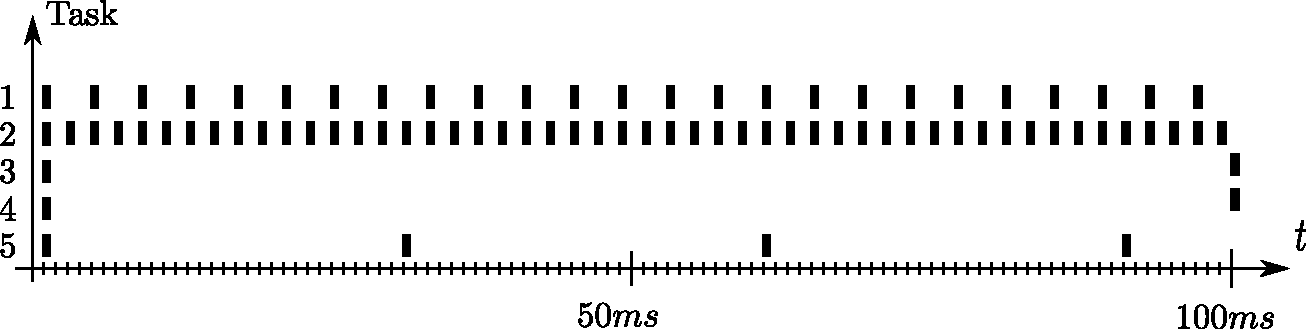
\includegraphics[scale=0.6]{figures/scheduleRequest.pdf}
	\caption{An overview of the tasks requests during 100ms.}
	\label{scheduleRequestd}
\end{figure}\vspace{-5mm}


When two task requests to run at the same time, the order is chosen according to the priorities, that are set at the initialisation. If the processor is free. the task are run when they ask for it, but interrupted when a higher priority task needs to run, and will finish when all the higher priority tasks are done. An example of this case can be seen in \figref{schedulePriorities}.\\
The priorities of the task have been made to give the system the best stability. In this case, The angular sensor has the highest priority because it has a large period and running time, but is critical to the steering of the vehicle which is the main objective of this project. Then comes the hall sensors that is very fast to execute, and then the speed control which is so fast that is not critical to have it at a high priority. The last one is the GoT system and communication protocol along with the distance control, because of two things: first because it may enter in an infinite loop and block the system if no data is received, and second and most of all because the main point of this project is to be able to run without the GoT system if something happens to block the communication.

 \begin{figure}[H]
	\centering
	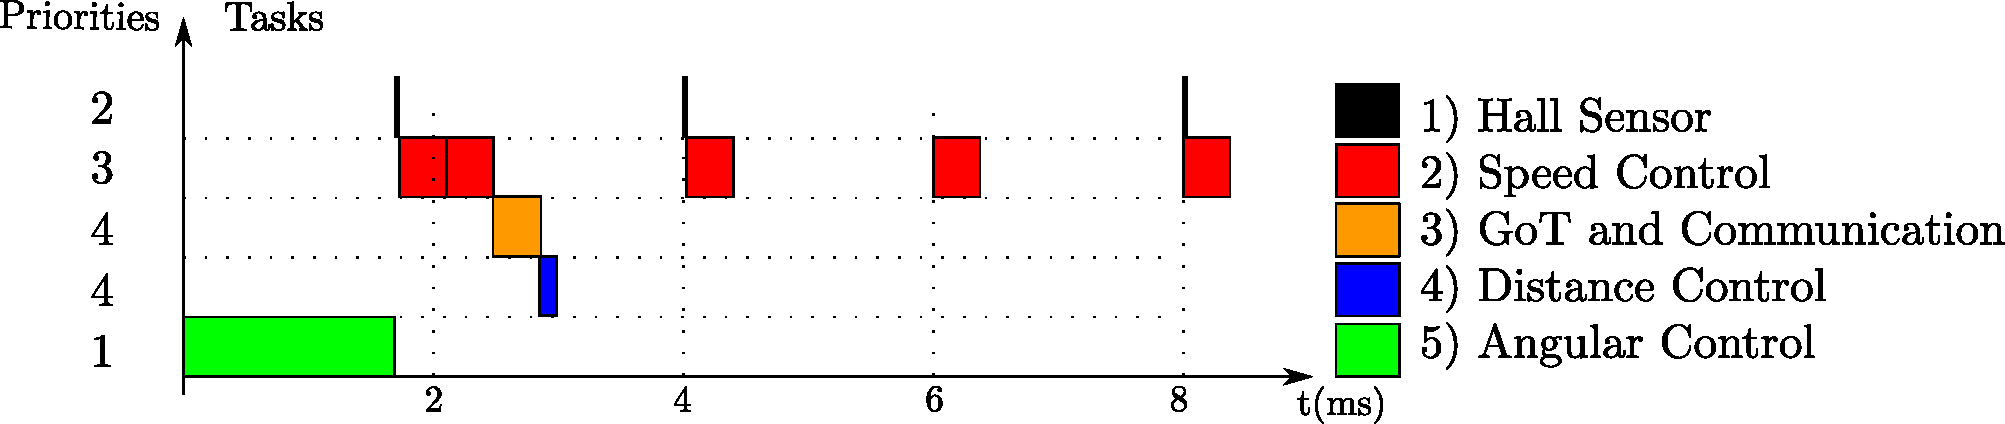
\includegraphics[scale=0.5]{figures/schedulePriorities.pdf}
	\caption{Schedule of the tasks at the starting time, regarding the priorities.}
	\label{schedulePriorities}
\end{figure}\vspace{-5mm}

As seen on the  \figref{schedulePriorities}, the angular control has the highest priority so it will run first, and the others will be registrered in a queue in order of priority. Then the hall sensors are second, and speed control after that. The GoT and comunication will run after them, and in the end the Distance Control.\\
After a certain time, the task running periods will stabilize, until the tasks with a large period are executed again.

Now that the hardware and software choices have been made, described and explained, the tasks for the sensors can be implemented, independently from each other.

%--------- Chapter 5 ----------------------------------------
\chapter{Sensor Implementation}\label{chap:sensorsImplementation}
The different sensors used in this project need some tuning from the software part to work as expected in a consistent way and give valuable data.\\
The next sections describe how this can be done both for the Hall sensors and the magnetometer.
\section{Hall-sensor}

The velocity calculation is done trough the Hall sensors. There are four magnets on the gear at approximatly a quarter of a turn of distance each. One way of getting the speed is by calculating the time between each outputs and the distance traveled during that time. A plot of the speed can be seen on \figref{unfilteredHall}.

\begin{figure}[H]
	\centering
	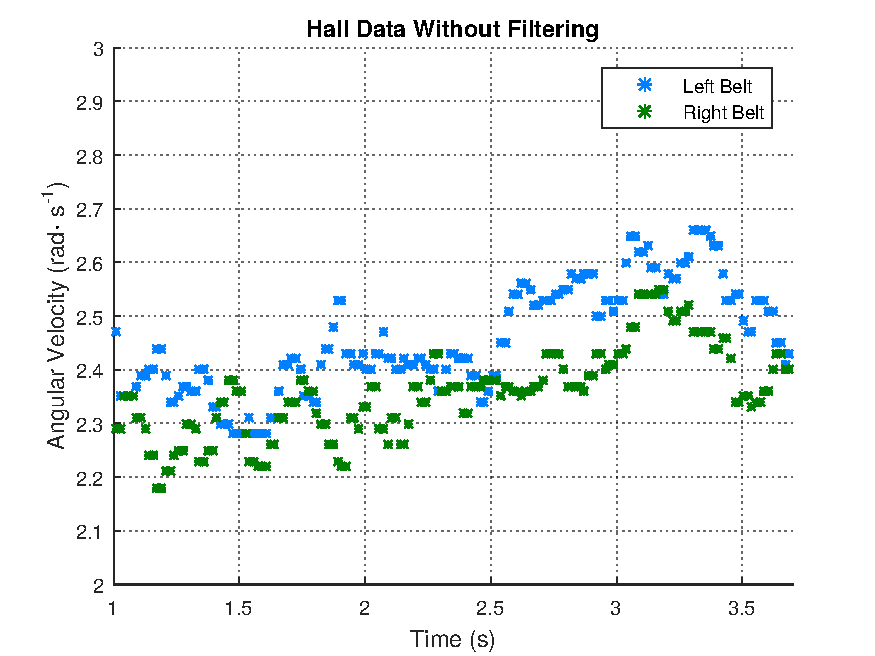
\includegraphics[scale=0.9]{figures/unfilteredHall.pdf}
	\caption{Plot of an unfiltered measurement by the Hall Sensors at full speed}
	\label{unfilteredHall}
\end{figure}


This is a plot of the speed, with unaccurate measurement because of the uneven placement of the magnets, with a calculation of the time between each magnets.\\


The new approach is to get the time the wheel take to make a full turn, to have the exact time and distance of a rotation. The speed will be calculated from a full turn every magnets, compared to the last time it was registered, four outputs before. A plot of the measurements can be seen on \figref{filteredHall}.

\begin{figure}[H]
	\centering
	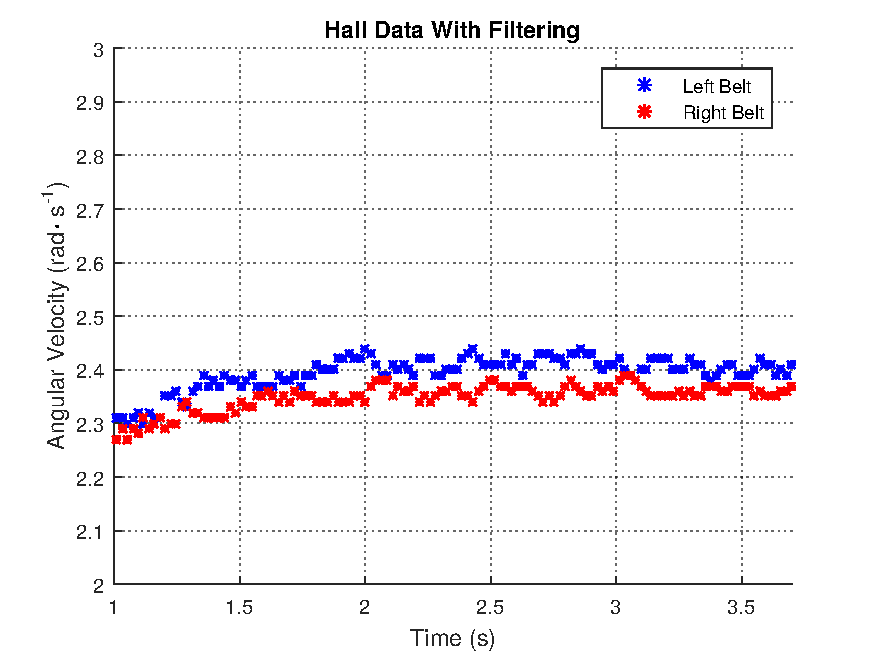
\includegraphics[scale=0.9]{figures/filteredHall.pdf}
	\caption{Plot of an filtered measurement by the Hall Sensors at full speed}
	\label{filteredHall}
\end{figure}

The difference between the two plots is that at constant speed, the time measured at each outputs is uneven on \figref{unfilteredHall}, and even in \figref{filteredHall}. A flowchart of the implementation of the functions of the Hall Sensors can be seen on \figref{hallFlowchart}.

\begin{figure}[H]
	\centering
	\includegraphics[scale=0.9]{figures/hallFlowchart.pdf}
	\caption{Flowchart of the two main functions \textit{tSpeed} and \textit{getSpeed} of the Hall Sensors implementation}
	\label{hallFlowchart}
\end{figure}

This flowchart explains the way of getting the time at each outputs. The Hall Sensors use the timers 4 and 5 to register the time of the output. The first function \textit{tSpeed} describes the storing of the two timers values in the registers, the second is a subfunction of the first one, and the last function \textit{getSpeed} is the calculation of the speed from the raw data of a variable in the function \textit{tSpeed}.\\


\subsubsection{Minimum speed because of the registers}



\subsubsection{FIR Filter}

Using the four magnets of the wheel and recording the time values through the timers involve using a  FIR Filter(Finite Impulse Response Filter). An overview of the filter can be seen on \figref{FIRFilter}.


\begin{figure}[H]
	\centering
	%\includegraphics[scale=0.9]{figures/FIRFilter.pdf}
	\caption{Overview of an FIR Filter}
	\label{FIRFilter}
\end{figure}
\section{Magnetometer}\label{sec:magnetoSensor}
The ``Sparkfun 9 degrees of freedom'' sensor board \cite{Sparkfun9D0F} used in this project includes three sensors, of which one is the magnetometer chip HMC5883L \cite{HMC5883L}. Since the Earth's magnetic field only moves slightly, it is possibe to neglect this movement from the sensor's point of view. The magnetometer uses this property to calculate the three space components (x,y,z) of the Earth's magnetic field magnitude, therefore indicating the North pole's position relative to the sensor's own orientation.\\
The coordinates are sent through \si{I^2C} each time asked by the software onboard the Arduino. This means that it is possible to set the sampling time according to the needs of the steering controller part, within the sensor's sampling limits. 
By maintaining the sensor in a horizontal position and using trigonometry it is possible to get an angle equivalent to a compass heading, with the North as a reference of \si{0^{\circ}} :
\begin{flalign}
\eq{\theta_{heading}}{\frac{180}{\pi} \cdot \arctan\left(-\frac{y}{x}\right)} \unit{^{\circ}}
\label{eq:headingTrigonometry}
\end{flalign}
\hspace{6mm} Where:\\
\begin{tabular}{p{1cm}lll}
& \si{\theta_{heading}} & is the sensor's heading                  		&\unitWh{^{\circ}}\\
& \si{\arctan} 			& is the reciprocal of the \si{\tan} function    &\unitWh{rad}\\
& \si{y} 				& is the y-component of the measured magnitude 	&\unitWh{G}\\
& \si{x} 			    & is the x-component of the measured magnitude 	&\unitWh{G}\\
\end{tabular}

In \eqref{eq:headingTrigonometry}, the angle calculated from the arctangent function is converted from radians to degrees to facilitate the work with angle orientations later in the code.
%
However, to be able to use the heading values received from the sensor and this formula, it is necessary to first calibrate the sensor \cite{JJankowski}. This allows the sensor to account for magnetic disturbances that could happen in its environment, see \appref{app:magnetoCalibration}. It might be possible though, that unpredictable disturbances occur during the mowing of the lawn. This is why a digital filtering approach is considered in \chapref{chap:digitalFilter}.

The sensors placed on the vehicle is up and running, now the coordinate from the GoT system should be set up, so the vehicle can utilize them.
\chapter{Communication}
A communication system is desired for transporting the GoT data, calculated to coordinates on the computer, to the microcontroller, located on the vehicle. Furthermore a protocol handling packet transitions is necessary to implement on top of the communication system to be able to fulfil requirements set in \secref{Requirements}.

\section{OSI model}
The Open Systems Interconnection, OSI, model is a standard used to describe how information moves in a network. Each layer describing standardization of what should occur in the specific layer \cite{Microsoft}. The seven layers of the OSI model is illustrated in \tableref{tab:OSIModel}.

\begin{table}[H]\centering
\begin{tabular}{|p{1.5cm}|p{3cm}|}
\hline%-----------------------------------------------------------------------------------------------------------------
  \textbf{Layer} & \textbf{OSI} \\
\hline%-----------------------------------------------------------------------------------------------------------------
    7 &    Application      \\
\hline%-----------------------------------------------------------------------------------------------------------------
    6 &    Presentation      \\
\hline%-----------------------------------------------------------------------------------------------------------------
    5 &    Session       \\
\hline%-----------------------------------------------------------------------------------------------------------------
    4 &    Transport    \\
\hline%-----------------------------------------------------------------------------------------------------------------
    3 &   Network     \\
\hline%-----------------------------------------------------------------------------------------------------------------
    2 &   Data link     \\
\hline%-----------------------------------------------------------------------------------------------------------------
    1 &    Physical     \\
\hline%-----------------------------------------------------------------------------------------------------------------
\end{tabular}
\caption{OSI model}
\label{tab:OSIModel}
\end{table}

The Physical layer is the electrical/mechanical hardware layer. The layer handles bits and determines what is a binary 0 and 1. The prototype utilizes two Xbee's, one in the computer and one on the vehicle, for the lowest layer of communication.

The Data link layer functionality ensures physical addressing, error control when transferring data between nodes over the physical layer, and access control \cite{J.M.Network}. The Data link layer is something the Xbee module handles to ensure that it transmits bytes correctly.

The Network layers main functionality is routing across a network. This is not utilized in the protocol. Since the communication is only between two Xbees, i.e. two nodes. 

The Transport layers handles package and has the ability to assemble or disassemble packages. An important part of the functionality of this layer is to ensure reliable transmission of data packages.

The layers above the transport layer is not utilized in the prototypes communication protocol. Since the session is more overall version of network and the presentation layer transforms the code into something application layer can utilize for user interface. These application is not needed when communicating between the computer and the vehicle, since no user interaction is implemented and a one-way communication between two units is utilized. 

\section{Protocol}
The main object for the communication system is to transmits the coordinates from the computer to the microcontroller. A transport layer protocol is created to ensure packets can be transmitted, receive, i.e. the needed information can be extracted from the packet, and be able to identify erroneous packets.

A connectionless system is implemented, since it is one-way communication, from the computer to the microcontroller and retransmission not desired, since the vehicle is moving and a retransmission of a coordinate will cause a delay. Additionally, the sampling rate of the GoT system i 10 \si{Hz}, so transmitting the recently received coordinates would be sufficient. Therefore is erroneous packages thrown away and acknowledgements is not utilized.

\subsection{Protocol Package Structure}
A package structure is desired for containing necessary information for addressing, decrypting and error handling. The protocol has an header which contains a start byte, a destination and the length of the package. The body of the package is the data and the tail is the checksum and the end byte. The package structure is illustrated in \tableref{CoorSetup}.

\begin{table}[H]\centering
\begin{tabular}{|>{\centering\arraybackslash}m{2cm}|>{\centering\arraybackslash}m{3cm}|>{\centering\arraybackslash}m{2cm}|>{\centering\arraybackslash}m{2cm}|>{\centering\arraybackslash}m{2cm}|>{\centering\arraybackslash}m{2cm}|}
\hline
Start Byte & Destination ID & length & Data & Checksum & End byte \\
\hline
\end{tabular}
\caption{The structure of a package}
\label{CoorSetup}
\end{table}

\subsubsection{Destination ID}
The Destination ID is to ensure packages, which is transmitted, is handled by the correct receiver. This way the transmitter can transmit to numerous receivers if multiple vehicles is utilized. The destination ID ensures the receivers can filter out packages not intended for them. The microcontroller has the destination ID 0000 0001. The length of the destination byte is set to one byte, so the destination can be read immediately when received.

UDP, a connectionless protocol, utilizes a source, but in this case it is not necessary, since only one computer is transmitting, the receiver does not need to know where the package has been transmitted from. Even if there more computers was utilized it would not be necessary as long as the package is marked with the destination ID, the receivers is able to read it. If retransmission was utilized, in case of erroneous packages, a source is necessary to have the ability to ask for a retransmission from the sender. Since retransmission is not utilized a source is not included in the package structure.

\subsubsection{Length}
The Length is utilized by the receiver. This will make it possible for the receiver to know the bit length of the package, and thereby know when the package should end. Each package created has the same length. The length is set to contain 7 bit, this can count up to $2^{7}-1 = 127$, which is sufficient.

\subsubsection{Data}
The data received from the GoT system consist of three coordinates (X,Y,Z), locating the position of the vehicle. Each of these coordinates can have a value from -9000 to 9000 (see \secref{GoTDescription}). To contain a number of this size, a 15 bit signed integer is utilized. Of the 15 bit 14 bit is utilized for the magnitude of the coordinate, which can have a value of 16385 ($2^{14}-1$). The last bit of the 15 bit is utilized to indicate if a coordinate is positive or negative, i.e. sign bit. The protocol is designed so the sign bit will be placed at the end of the 15 bit integer. As both the microcontroller and the computer utilizes little endians, there will not be a problem with the transmission of numbers. With little endians, the bit with the highest value will be located next to the sign bit and the bit with the lowest value is located at the beginning of the bit array. This will yield the bit array illustrated on \tableref{CoorSetup}.

\begin{table}[H]
\centering
\begin{tabular}{|>{\centering\arraybackslash}m{0.5cm}|>{\centering\arraybackslash}m{0.5cm}|>{\centering\arraybackslash}m{0.5cm}|>{\centering\arraybackslash}m{0.5cm}|>{\centering\arraybackslash}m{0.5cm}|>{\centering\arraybackslash}m{0.5cm}|>{\centering\arraybackslash}m{0.5cm}|>{\centering\arraybackslash}m{0.5cm}|>{\centering\arraybackslash}m{0.5cm}|>{\centering\arraybackslash}m{0.5cm}|>{\centering\arraybackslash}m{0.5cm}|>{\centering\arraybackslash}m{0.5cm}|>{\centering\arraybackslash}m{0.5cm}|>{\centering\arraybackslash}m{0.5cm}|>{\centering\arraybackslash}m{0.65cm}|}
\multicolumn{15}{c}{15 bits} \\
\hline
$2^0$ & $2^1$ & $2^2$ & $2^3$ & $2^4$ & $2^5$ & $2^6$ & $2^7$ & $2^8$ & $2^9$ & $2^{10}$ & $2^{11}$ & $2^{12}$ & $2^{13}$ & $+/-$ \\
\hline
\end{tabular}
\caption{Setup for the bit array, that contains one of the coordinate values.}
\label{CoorSetup}
\end{table}

The representation of the integer is called signed magnitude. Another representation that could be used is ones' complement. Here the number is inverted if the signed bit is true. But for an easier implementation on the computer, the signed magnitude is utilized. The code firsts checks if the number is positive or negative. If negative, the sign bit is set and the number is multiplied by minus one, this will yield the magnitude. The magnitude is then converted into a bit array. When converting back, it is only necessary to multiply the magnitude by minus one, if the sign bit is true.

\subsubsection{Checksum}
To ensure package data is received correctly, error handling is added to the protocol. A error handling which is utilized is a checksum. The way the checksum is calculated, is by splitting the header and the data up into pieces of equal size and then summing the pieces together. The summed bit array is then inverted and the remaining bit array is the checksum. 

there is 60 bit in the header and the data combined, i.e. 15 per coordinate, 8 for the destination and 7 for the length. these will be split up into three pieces of 20 bit. The related checksum consist of 20 bit. Combined, the header, data and checksum is 80 bit, which is equal to 10 bytes. In \tableref{ChecksumExp} an example of calculating a checksum is given.

\begin{table}[H]
\centering
\begin{tabular}{c c c c c c c c c c c}
   & Bit array  &     & Decimal &     & Bit 0-3 & Bit 4-7 & Bit 8-11 & Bit 12-15 & Bit 16-19 & Bit 20 \\
\hline
a) & Part 1     & $=$ & 123008  & $=$ & 0000 & 0001 & 0000 & 0111 & 1000 & \\
b) & Part 2     & $=$ & 351365  & $=$ & 1010 & 0001 & 0011 & 1010 & 1010 & \\
c) & Part 3     & $=$ & 729671  & $=$ & 1110 & 0010 & 0100 & 0100 & 1101 & \\
d) & Part 1+2+3 & $=$ & 1204044 & $=$ & 0011 & 0010 & 1111 & 1010 & 0100 & 1 \\
e) & Add carry  & $=$ & 155469  & $=$ & 1011 & 0010 & 1111 & 1010 & 0100 & \\
f) & Checksum   & $=$ & 893106  & $=$ & 0100 & 1101 & 0000 & 0101 & 1011 & \\
g) & Check      & $=$ & 1048575 & $=$ & 1111 & 1111 & 1111 & 1111 & 1111 & \\
\end{tabular}
\caption{The pieces consisting of the destination ??, length with the value of 96, and the data which is 4259, 7511 and -6418.}
\label{ChecksumExp}
\end{table}

The three pieces is added together, the destination, length and the data (see on line d). This produces a carry, since the checksum has the size of 20 bit. The carry is added to the beginning of the sum (see on line e). The generated sum is then inverted to yield a checksum (sees on line f).

When the receiver utilizes the checksum needs to check if the destination, length and data corresponds with the related checksum. The checksum is first added together with the three 20 bit pieces and, if there is any, the carry. If the outcome of the bit summation results in 20 bits which are true, then the package is received correctly. If not, the receiver will throw away the package. An error in the received package could be a bit inversion or some data not received by the receiver. 

A flaw when utilizing the created checksum, is that an error can cancelled out another error, and thereby make some errors undetectable. This can happen when the system adds the three pieces and the checksum together. An example, is if the first bit in piece number one is true and the first bit in piece number two is false. If both of these bits are shifted independently, so the bit from part one become false and the bit in part two true, the checksum can not detect the error. The likelihood for this to happen is very slim, as the errors first have to occur and then they have to be located a place where they cancel each other out. Having only 4 pieces of 20 bits, the likelihood of this happening is lesser than if the checksum was set to 10 bit. Since the addition occurs with 7 pieces of 10 bit. This would yield more bits with the same rank, so there would be a higher possibility for a bit cancelling each other out. This is a good argument for utilizing a larger checksum, even if it uses more space.

\subsubsection{Start and end byte}
As the computer transmits a package each time it receives coordinates from the GoT system, a queue of packages can appear in the microcontroller, packages handling is to slow. To not make the system able to differentiate packages from each other a start byte is added at the beginning of the package and an end byte at the end of the package. 

To find the start of a package the system will search for a start byte. When finding the start byte, it will read the destination, length, data and checksum and then look for a end byte. If the end byte is not found at that point, then the package is not received correctly and is thrown away. If the end byte is found, then system utilize the package and apply error handling on it. 

The start byte is set to 0000 1111. This is chosen to ensure the start byte does not have an identical value with another byte in the header. This is done to ensure no misunderstandings occurs. The end byte will come just before the next start byte, there is the value of the end byte inverted compared to the start byte, this yields an end byte of 1111 0000.

With the destination, length, data, checksum, start and end byte has been describe and a final package structure is illustration in \tableref{PackageLook}

\begin{table}[H]
\centering
\begin{tabular}{|c|c|>{\centering\arraybackslash}m{0.3cm}|>{\centering\arraybackslash}m{0.3cm}|>{\centering\arraybackslash}m{0.3cm}|>{\centering\arraybackslash}m{0.3cm}|>{\centering\arraybackslash}m{0.3cm}|>{\centering\arraybackslash}m{0.3cm}|>{\centering\arraybackslash}m{0.3cm}|>{\centering\arraybackslash}m{0.3cm}|>{\centering\arraybackslash}m{0.3cm}|>{\centering\arraybackslash}m{0.3cm}|>{\centering\arraybackslash}m{0.3cm}|>{\centering\arraybackslash}m{0.3cm}|>{\centering\arraybackslash}m{0.3cm}|>{\centering\arraybackslash}m{0.3cm}|>{\centering\arraybackslash}m{0.3cm}|>{\centering\arraybackslash}m{0.3cm}|}
\hline
\multicolumn{2}{|c|}{Offsets} & \multicolumn{8}{c}{Byte 1} & \multicolumn{8}{|c|}{Byte 2} \\
\hline
\multicolumn{1}{|c}{Byte} & \multicolumn{1}{|c|}{Bit} & 0 & 1 & 2 & 3 & 4 & 5 & 6 & 7 & 8 & 9 & 10 & 11 & 12 & 13 & 14 & 15 \\
\hline
0 & 0 & \multicolumn{8}{c}{Start byte} & \multicolumn{8}{|c|}{Destination} \\
\hline
2 & 16 & \multicolumn{7}{c}{Length} & \multicolumn{9}{|c|}{X coordinate} \\
\hline
4 & 32 & \multicolumn{6}{c}{X coordinate} & \multicolumn{10}{|c|}{Y coordinate} \\
\hline
6 & 48 & \multicolumn{5}{c}{Y coordinate} & \multicolumn{11}{|c|}{Z coordinate} \\
\hline
8 & 64 & \multicolumn{4}{c}{Z coordinate} & \multicolumn{12}{|c|}{Checksum} \\
\hline
10 & 80 & \multicolumn{8}{c}{Checksum} & \multicolumn{8}{|c|}{End byte} \\
\hline
\end{tabular}
\caption{Illustration of a package, that will be send from the transmitter to the receiver.}
\label{PackageLook}
\end{table}

This yields a package with a length of 96 bit (12 byte). As the GoT system have a sampling frequency of 10 Hertz and each sampling gives out 12 byte, the transfer speed for the Xbee have to be greater than 120 byte per second, which it is \secref{Hardwarechoice}.

\subsubsection{Further Error Handling}
A package can be damaged when it is transmitted from the computer to the microcontroller or a byte in the coordinate could have a identical value with the start or end byte. for example, if a packet has a byte of the coordinate with the same value as the start byte, the start of a package could be registered in the middle of a package. To detect this and further damages in which the checksum is not able to register, extra error handling is utilized. The receiving process is illustrated in \figref{FlowReceiver}.

\begin{figure}[H]
\centering
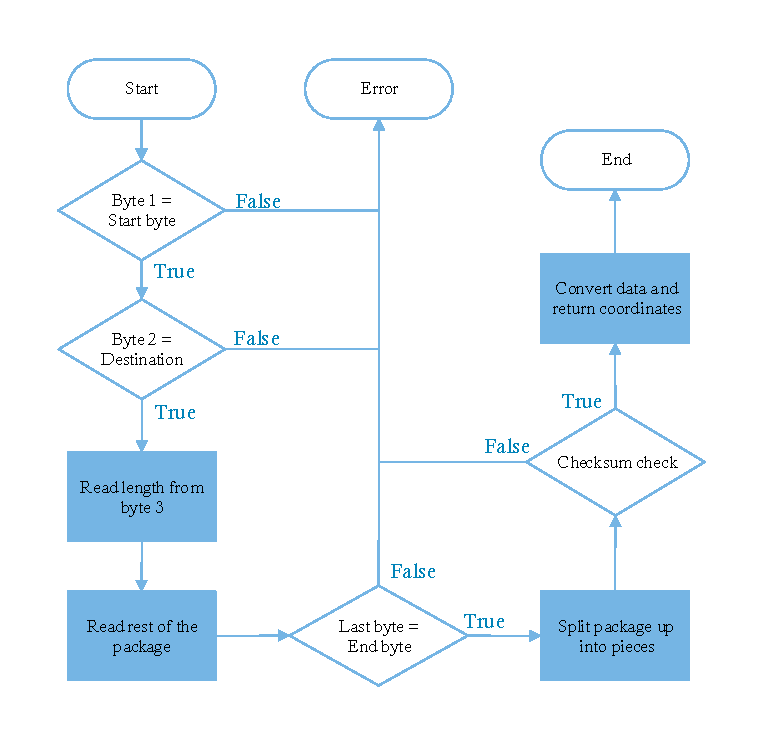
\includegraphics[scale=1.2]{figures/FlowReceiver.pdf}
\caption{Flow chart over the error handling in the receiver part.}
\label{FlowReceiver}
\end{figure}

If the package is transmitted correctly, the 1st byte received is the start byte and the 2nd byte is the destination ID of the receiver. The 3rd byte will contain 7 bit for the length and 1 bit for the first coordinate. If the length is without errors its value would be 96, which is 12 byte. The last byte, the 12th one, is the end byte. If these condition are all correct, the receiver will check for errors utilizing the checksum. If that checksum is also correct, the system will convert the data and return the coordinates to the rest of the system.

If an error occurs, then all the bytes that have been read will be thrown away. Thus throwing the whole package away even if the start byte and the destination are correct, but the end byte is not. If the start byte is not correct, then only that byte will be thrown away until finding a correct start byte. This method is applied to ensure the system only utilizes complete packages.

This prevents the receiver to start in the middle of a package, as the system will throw away incomplete or damaged packages, until it finds a start byte. One example when utilizing this feature can cause a problem. If a start byte has a identical value with a byte in data or checksum. The problem will occur if the second byte is equal to the receivers destination ID, and the first seven bits of the next byte are equal to 96, which is the value of the length. An example on a situation where this problem occurs is illustrated in \tableref{errorPro}.

\begin{table}[H]
\centering
\begin{tabular}{c | m{0.1cm} m{0.1cm} m{0.1cm} m{0.1cm} m{0.1cm} m{0.1cm} m{0.1cm} m{0.1cm} | c | m{0.1cm} m{0.1cm} m{0.1cm} m{0.1cm} m{0.1cm} m{0.1cm} m{0.1cm} m{0.1cm} | l }
\multicolumn{9}{c}{Normal reading} & \multicolumn{9}{c}{Displaced reading} &  \\
\cline{2-9} \cline{11-18}
1st byte & 0 & 0 & 0 & 0 & 1 & 1 & 1 & 1 & 5th byte & 0 & 0 & 0 & 0 & 1 & 1 & 1 & 1 & $\leftarrow$ Start byte \\
\cline{2-9} \cline{11-18}
2nd byte & 0 & 0 & 0 & 0 & 0 & 0 & 0 & 1 & 6th byte & 0 & 0 & 0 & 0 & 0 & 0 & 0 & 1 & $\leftarrow$ Destination \\
\cline{2-9} \cline{11-18}
3rd byte & 0 & 0 & 0 & 0 & 0 & 1 & 1 & 0 & 7th byte & 0 & 0 & 0 & 0 & 0 & 1 & 1 & 0 & $\leftarrow$ Length (First seven bit)\\
\cline{2-9} \cline{11-18}
4th byte & 1 & 1 & 1 & 1 & 0 & 0 & 0 & 0 & 8th byte & 0 & 1 & 1 & 1 & 0 & 0 & 1 & 1 & \\
\cline{2-9} \cline{11-18}
5th byte & 0 & 0 & 0 & 0 & 1 & 1 & 1 & 1 & 9th byte & 1 & 0 & 0 & 1 & 1 & 0 & 1 & 1 & \\
\cline{2-9} \cline{11-18}
6th byte & 0 & 0 & 0 & 0 & 0 & 0 & 0 & 1 & 10th byte & 1 & 0 & 0 & 0 & 0 & 1 & 0 & 0 & \\
\cline{2-9} \cline{11-18}
7th byte & 0 & 0 & 0 & 0 & 0 & 1 & 1 & 0 & 11th byte & 0 & 0 & 1 & 1 & 0 & 1 & 1 & 1 & \\
\cline{2-9} \cline{11-18}
8th byte & 0 & 1 & 1 & 1 & 0 & 0 & 1 & 1 & 12th byte & 1 & 1 & 1 & 1 & 0 & 0 & 0 & 0 & \\
\cline{2-9} \cline{11-18}
9th byte & 1 & 0 & 0 & 1 & 1 & 0 & 1 & 1 & 1st byte & 0 & 0 & 0 & 0 & 1 & 1 & 1 & 1 & \\
\cline{2-9} \cline{11-18}
10th byte & 1 & 0 & 0 & 0 & 0 & 1 & 0 & 0 & 2nd byte & 0 & 0 & 0 & 0 & 0 & 0 & 0 & 1 & \\
\cline{2-9} \cline{11-18}
11th byte & 0 & 0 & 1 & 1 & 0 & 1 & 1 & 1 & 3rd byte & 0 & 0 & 0 & 0 & 0 & 1 & 1 & 0 & \\
\cline{2-9} \cline{11-18}
12th byte & 1 & 1 & 1 & 1 & 0 & 0 & 0 & 0 & 4th byte & 1 & 1 & 1 & 1 & 0 & 0 & 0 & 0 & $\leftarrow$ End byte\\
\cline{2-9} \cline{11-18}
\end{tabular}
\caption{Example of a normal reading of a package and a displaced reading of a package. The package contains the coordinates (-8222, 515, -3699).}
\label{errorPro}
\end{table}

In the example illustrated in \tableref{errorPro}, the 5th to 7th byte are equal to the start byte and the header. If the system is searching for the start byte and finds the 5th byte, it will begin to search for the header. In this case it will find it and as the 12th byte, which is in the next package, is equal to the end byte, the system will confirm it as a complete package. But since a checksum is implemented, it will be unlikely if the package is confirmed. The checksum, in this case, will not be the original checksum for the package, but another part of the package. As this checksum is not calculated to fit, the likelihood for the check going through is so poor, that error handling detecting this is not implemented. 

If a erroneous package is being stopped by the checksum, the 12 bytes would still have been read and is therefore thrown away. In the 12 bytes thrown away a correct start byte can be located. A problem can occur if the next three bytes, after the 12 bytes which is thrown away, is equal to the start byte and header again. Then the same scenario will repeat it self and will continue, until the three byte no longer equals the start byte and header. The scenario is unlikely, as three bytes has to be identical to the start byte and the header. 

The transport layer protocol implemented on top of the Xbee modules has now been described.


\section{Communication Filtering}
The GoT system gives the vehicle's position throughout time. However, since this system use ultrasound waves to register positions in space, it can easily be distorted by interferences and objects on the wave path. It is therefore required to eliminate the big jumps in positions, that could happen in the GoT system, before sending them to the vehicle, see \chapref{Requirements}.

Since the vehicle cannot run faster than \si{3,0\ m \cdot s^{-1}} and that the chosen velocity for the velocity controller is \si{1,4\ m \cdot s^{-1}}, it is possible to define a certain range of positions for a defined time interval. This range is define as a circle, with the a radius as large as the assumed maximum velocity, set to \si{3,0\ m.s^{-1}}, multiplied with the measurement time interval. An example with a \si{1\ s} time interval is given on \figref{GoTFilterSimple}.
\begin{figure}[H]
  \centering
  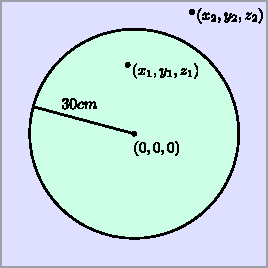
\includegraphics[scale=0.6]{figures/GoTFilterSimple.pdf}
  \caption{Range of possible positions for a maximum speed of \si{3,0\ m \cdot s^{-1}} during a \si{1\ s} interval}
  \label{GoTFilterSimple}
\end{figure}
If the position at a given time, \si{t_0} is \si{(0,0,0)}, the coordinates at the next measurement time, \si{t_1\ =\ t_0\ +\ 1\ s}, should stay within a \si{3,0\ m} radius of the first position.

To ensure the fact that no position jumps is sent to the vehicle, its velocity is measured from the two last sets of coordinates (converted from \si{mm} to \si{m}) and the sampling time of the GoT system (\si{100\ m \cdot s^{-1}}, see \secref{GoTDescription}), see \eqref{eq:velocityGoTCalc}.
\begin{flalign}
\eq{v}{\frac{\sqrt{(X_{2} - X_{{1}})^2 + (Y_{2} - Y_{{1}})^2 + (Z_{2} - Z_{{1}})^2}}{\Delta T}}\unit{m \cdot s^{-1}}
\label{eq:velocityGoTCalc}
\end{flalign}
\hspace{6mm} Where:\\
\begin{tabular}{p{1cm}lll}
  &\si{v}                   & is the velocity of the vehicle                      &\unitWh{m \cdot s^{-1} }\\
  &\si{(X_{2},Y_{2},Z_{2})}   & is the the last set of measured coordinates         &\unitWh{m}\\
  &\si{(X_{1},Y_{1},Z_{1})}   & is the the second last set of measured coordinates  &\unitWh{m}\\
  &\si{\Delta T}            & is the sampling time                                &\unitWh{s}\\
\end{tabular}

Whenever a calculated velocity is greater than the limit of \si{3,0\ m \cdot s^{-1}}, the newest set of coordinates is completely discarded. To calculate the newest velocity afterwards, the previous position, that was not discarded, and the newly measured position are taken, and the sampling time is extended by \si{100\ m \cdot s^{-1}} until a velocity under the limit is measured. When the velocity is under the limit again, the time interval is set to default value again.

However, this type of inconsistency in the system should be fairly rare at a speed of \si{1,4\ m \cdot s^{-1}}, as this so much slower than the limit, which then never will be discarded. And with the GoT is correctly calibrated and the vehicle's environment is clear of interfering obstacles, the distributions will occur rarely and not inflect hard on the system. 	

%---------- Chapter 6 ---------------------------------------- Modelling of the Vehicle
\chapter{Modeling of the Vehicle}\label{cha:ModelOfVehicle}

The prototype model contains software, hardware and mechanical components. Software and hardware components are easy to change and to model after how the rest of the system is made and shall run. The vehicle, which is a mechanical plant, is provided to this project and therefore not changeable. This means that requirements about how the system should react, described in \secref{sec:Vehicledescription}, apply only for elements of the system that are external to the plant. In this chapter, a model of the vehicle is made to describe the power transfer from both the motor's and servomotor's rotational energy to the movement of the vehicle. Once, this model is established, it is possible to measure its output and apply a control on it, see \chapref{cha:ControlOfTheVehicle}.


\begin{figure}[H]
	\centering
	\includegraphics[width=\textwidth]{figures/completeMechanical.pdf}
	\caption{A mechanical diagram of the vehicle}
	\label{fig:completeMechanicalDiagram}
\end{figure}

The \figref{fig:completeMechanicalDiagram} shows both the drivetrain and steering mechanisms on the given vehicle. It is possible to identify and separate these two sub-systems. The driving part allows the vehicle to run and comprises the motor, all the gears that make the belts turn and the belts themselves. On the other hand, the steering part is made of the servomotor which acts on two shafts and breaks one or the other belt, as stated in \secref{sec:Vehicledescription}. In the next sections, the drivetrain, which allows the vehicle to run, and the steering part, which allows the vehicle to turn, are modelled separately, and eventually recombined into a single model.
\section{Velocity model}
This section will contain the modelling of the car.

Plant that we were given, to be able to make requirements.

Black boxing:


\begin{figure}[H]
	\centering
	\includegraphics[scale=0.6]{figures/StartTotalModelsystem.pdf}
	\caption{}
	\label{fig:StartTotalModelsystem}
\end{figure}

\subsection{Motor Modelling}\label{motormodelling}
In this section a model of a motor is depicted only as an electrical system, which delivers a rotational force called torque, \si{\tau_m}. The electrical model provides the motor's produced torque to the drivetrain which is further discussed in \secref{DriveTrain}.
%
\subsubsection{Electrical Model}
The output needed from the motor's electrical model is the torque, \si{\tau_m}. To obtain the torque, the formula for translating the electrical current, \si{i_a}, to torque is utilized:
%
\begin{flalign}\centering
  \eq{\tau_m(t)}{K_t \cdot i_a(t)} \unit{N \cdot m}
  \label{equ:motortorque}
\end{flalign}
\hspace{6mm} Where:\\
\begin{tabular}{p{1cm}lll}
& \si{\tau_m(t)} & is the rotational force torque &\unitWh{N \cdot m} \\
& \si{i_a(t)} & is the electrical closed loop current &\unitWh{A}\\
& \si{K_t} & is the motor constant &\unitWh{N \cdot m \cdot A^{-1}}
\end{tabular}

An expression for the current, \si{i_a(t)}, is required to derive a model for the electrical system. In \figref{fig:electricaldiagrammotor} an electrical diagram of the motor is displayed.
%
\begin{figure}[H]
\centering
	\begin{circuitikz}[american voltages]
		\draw
		
		% electromotive force 
		(0,0) to [short] (6,0)
		%to [sV, l=$e_b$] (6,2) %  voltage
		(6,0) to [V, l=$e_b$] (6,3)
		%to node[short]{}(6,2)

		%to node[short]{}(0,0)		 
		(0,0) to [V, l=$U_a$] (0,3) %  voltage

		
		%to [R, l=$Z_G$] (3,3) % generator impedance
		
		(0,3) to [R, l_=$R_a$, i>_=$i_a$] (3,3)	
		
		to [L, l_=$L_a$] (6,3); 
	\end{circuitikz}
  \caption{A electrical diagram of the motor}
  \label{fig:electricaldiagrammotor}
\end{figure}
%
By using Kirchoff voltage law on the closed loop, seen in \figref{fig:electricaldiagrammotor}, an expression including $i_a$ can be derived:
%
\begin{flalign}
\eq{U_a(t)}{R_a \cdot i_a(t) + L_a \cdot \frac{di_a(t)}{dt} + e_b(t)}\unit{V} 
\label{MotorClosedLoop}
\end{flalign}
\hspace{6mm} Where:\\
\begin{tabular}{p{1cm}lll}
& \si{U_a(t)} & is the supply voltage                       &\unitWh{V} \\
& \si{R_a}    & is the internal resistance in the motor     &\unitWh{\Omega}\\
& \si{L_a}    & is the inductance in the motor              &\unitWh{H} \\
& \si{e_b}    & is the electromotive force, also called EMF &\unitWh{V} \\
\end{tabular}

The electromotive force, \si{e_b(t)}, is equivalent to:
%
\begin{flalign}
\eq{e_b(t)}{K_e \cdot \dot{\theta}_m(t)}\unit{V} 
\end{flalign}
\hspace{6mm} Where:\\
\begin{tabular}{p{1cm}lll}
& \si{K_e}            & is the electromotive constant        &\unitWh{Wb} \\
& \si{\dot{\theta}_m(t)} & is the angular velocity in the motor &\unitWh{rad \cdot s^{-1}} \\
\end{tabular}

The equivalent for the electromotive force is substituted into \eqref{MotorClosedLoop}.
%
\begin{flalign}
\eq{U_a(t)}{R_a \cdot i_a(t) + L_a \cdot \frac{di_a}{dt} + K_e \cdot \dot{\theta}_m(t)}&
\end{flalign}
%
The Laplace transform is applied to the derived equation:
%
\begin{flalign}
\eq{U_a(s)}{R_a \cdot i_a(s) + L_a \cdot s \cdot i_a(s) + K_e \cdot \omega_m(s)}&
\end{flalign}
%
The equation is solved for \si{i_a}:
%
\begin{flalign}
\eq{i_a(s)}{\frac{U_a(s) - K_e \cdot \omega_m(s)}{L_a \cdot s + R_a}}&
\end{flalign}
%
By substituting the derived equation for $i_a$ into \eqref{equ:motortorque}, a new expression for the motor's torque is derived. 
%
\begin{flalign}
\eq{\tau_m}{K_t \cdot i_a(s)}&\nonumber\\
\eq{\tau_m}{K_t \cdot \frac{U_a(s) - K_e \cdot \omega_m(s)}{L_a \cdot s + R_a}}
  \label{eq:Totaltorquewithcurrentexpression}
\end{flalign}
%
By dividing with the voltage applied to the motor, $U_a$, a relation can be established:
%
\begin{flalign}
\eq{\frac{\tau_m}{U_a(s) - K_e \cdot \omega_m(s)}}{\frac{K_t}{L_a \cdot s + R_a}}&
  \label{eq:TotaltorquewithcurrentexpressionTransferFunction}
\end{flalign}
%
A relation for the electrical model relative to the motor's torque has been derived. Thus enabling setting up calculations for the vehicle's drivetrain.
\subsection{Drivetrain}\label{Drivetrain}

%% INTRODUCTION %%
The drive train on the given belt vehicle is what translates the torque $\tau_m$ given by the motor into the actual movement of the vehicle. The model of this system part shows the relation between the applied rotational force (or torque) $\tau_m$ and the speed of the belts. It is still considered that the vehicle's tajectory follows a straight line.\\\\
%
Different iterations of this model can be made to get more acuraccy. The first of these iterations should give an overview of how the system reacts to a given torque input. 

%% SSSECTION : BLACK BOX MODEL %%
\subsubsection{Black Box Model}\label{BlackBoxModel}
To get a rough approximation of how the drive train works, a black box model is used. There is a small gear $G_m$ on the motor shaft, which is in contact with another actual gear $G_2$. The imaginary gear $G_d$ represents the differential and the gears and shafts of the drivetrain from (and including) this second gear $G_2$ to the gears that drive the belt, see \figref{fig:DrivetrainMechanicalModel} and \figref{fig:BeltMechanicalDiagram}. The number of teeths on $G_d$ is set to the total gear ratio of this black box

\begin{figure}[H]
	\centering
	\includegraphics[scale=0.8]{figures/mechanicalDrawing.pdf}
	\caption{A simple mechanical diagram of the vehicle drivetrain}
	\label{fig:DrivetrainMechanicalModel}
\end{figure}
\todo{Add notations to the diagram and create free body diagrams of belt and black box parts}

% APPLICATION OF NEWTON'S SECOND LAW %

\begin{figure}[H]
	\centering
	%\includegraphics[scale=0.8]{figures/mechanicalDrawing.pdf}
	\caption{A free body diagram of the motor gear}
	\label{fig:MotorGearFreeBodyDiagram}
\end{figure}

\begin{figure}[H]
	\centering
	%\includegraphics[scale=0.8]{figures/mechanicalDrawing.pdf}
	\caption{A free body diagram of the `black box' gear}
	\label{fig:BlackBoxGearFreeBodyDiagram}
\end{figure}

The \todo{cite equation with label eq:MotorMechaModel from motor modeling part}[EQUATION] is extended with the contribution of the load which is the whole drivetrain. Therefore, from \figref{fig:MotorGearFreeBodyDiagram} and Newton's second law appplied to rotational systems, the following equation can be extracted:
\begin{flalign}\centering
J_m \cdot \dot{\omega}_m(t) = \tau_m(t) - B_m \cdot \omega_m(t) - N_m \cdot f_c(t) 
\label{eq:MotorGearNewtonSecLaw}
\end{flalign}
\hspace{6mm} Where:\\
\begin{tabular}{p{1cm}ll}
& $J_m$ 			      & is the motor's inertia [$kg \cdot m^2$] \\
& $\omega_m$        & is the angular velocity of the motor [$rad \cdot s^{-1}$] \\
& $\dot{\omega}_m$ 	& is the angular acceleration of the motor [$rad \cdot s^{-2}$] \\
& $\tau_m$ 		     	& is the torque delivered by the motor [$N \cdot m$] \\
& $B_m$             & is the coefficient of the friction happening inside the motor [$N \cdot m \cdot s \cdot rad^{-1}$] \\
& $N_m$             & is the number of teeth of the motor gear $G_m$ [$number\ of\ teeths$] \\
& $f_c$             & is the coefficient of the contact force between $G_m$ and $G_d$ [$N \cdot m \cdot number\ of\ teeths^{-1}$]
\end{tabular}

The equation for \figref{fig:BlackBoxGearFreeBodyDiagram} is obtained the same way:
\begin{flalign}\centering
J_d \cdot \dot{\omega}_d(t) = N_d \cdot f_c(t) - N_d \cdot f_b(t)
\label{eq:BlackBoxGearNewtonSecLaw}
\end{flalign}
\hspace{6mm} Where:\\
\begin{tabular}{p{1cm}ll}
& $J_d$ 			      & is the `black box' gear inertia [$kg \cdot m^2$] \\
& $\omega_d$        & is the angular velocity of the `black box' gear [$rad \cdot s^{-1}$] \\
& $\dot{\omega}_d$ 	& is the angular acceleration of the `black box' gear [$rad \cdot s^{-2}$] \\
& $N_d$ 		     		& is the number of teeth on the `black box' gear [$number\ of\ teeth$] \\
& $f_b$             & is the coefficient of the contact force between $G_d$ and the belt [$N \cdot m \cdot number\ of\ teeths^{-1}$] \\
\end{tabular}

%% SSSECTION : BELT MODEL %%
\subsubsection{Belt Model}\label{BeltModel}

\begin{figure}[H]
	\centering
	\includegraphics[scale=0.8]{figures/mechanicalDrawingBelt.pdf}
	\caption{A mechanical diagram of the belt part}
	\label{fig:BeltMechanicalDiagram}
\end{figure}

\begin{figure}[H]
	\centering
	% \includegraphics[scale=0.8]{figures/mechanicalDrawingBelt.pdf}
	\caption{A free body diagram of the belt driven mass}
	\label{fig:BeltFreeBodyDiagram}
\end{figure}

From \figref{fig:BeltFreeBodyDiagram}, the mechanical equation of the belt system on \figref{fig:BeltFreeBodyDiagram} is found to be:
\begin{flalign}\centering
M \cdot \dot{v}(t) = r_t \cdot f_b(t) - B_{sys} \cdot v(t)
\label{eq:BeltMassNewtonSecLaw}
\end{flalign}
\hspace{6mm} Where:\\
\begin{tabular}{p{1cm}ll}
& $M$ 			  & is the vehicle's total weight [$kg$] \\
& $v$        	& is the linear velocity of the behicle [$m \cdot s^{-1}$] \\
& $\dot{v}$ 	& is the linear acceleration of the vehicle [$m \cdot s^{-2}$] \\
& $r_t$ 		  & is the translational coefficient between the last gear and the belt [$m \cdot number\ of\ teeths^{-1}$] \\
& $B_{sys}$   & is the coefficient of the friction happening throughout the gears [$N \cdot s \cdot rad^{-1}$] \\
\end{tabular}

The assembling of a model for the drivetrain is made from these separate mechanical equations.

% SSSECTION : ASSEMBLING OF THE DIFFERENT EQUATIONS %
\subsubsection{Drivetrain modeling}\label{DrivetrainModeling}
The combination of \eqref{eq:MotorGearNewtonSecLaw}, \eqref{eq:BlackBoxGearNewtonSecLaw} and \eqref{eq:BeltMassNewtonSecLaw} makes it possible to get the linear velocity of the vehicle $v$ out of the torque $\tau_m$ given by the motor. Indeed, it is possible to link these equations throughout the contact force coefficients $f_c$ and $f_b$.\\\\
%
Taking the Laplace-transform of these equations helps arranging them and eventually, to find a transfer function from $\tau_m(s)$ to $V(s)$ :
%
\begin{flalign}\centering
\eqref{eq:MotorGearNewtonSecLaw} \xRightarrow{\mathcal{L}} J_m \cdot s \cdot \omega_m(s) = \tau_m(s) - B_m \cdot \omega_m(s) - N_m \cdot F_c(s) 
\label{eq:MotorGearNewtonSecLawLaplace}
\end{flalign}
%
\begin{flalign}\centering
\eqref{eq:BlackBoxGearNewtonSecLaw} \xRightarrow{\mathcal{L}} J_d \cdot s \cdot \omega_d(s) = N_d \cdot F_c(s) - N_d \cdot F_b(s)
\label{eq:BlackBoxGearNewtonSecLawLaplace}
\end{flalign}
%
\begin{flalign}\centering
\eqref{eq:BeltMassNewtonSecLaw} \xRightarrow{\mathcal{L}} M \cdot s \cdot V(s) = r_t \cdot F_b(s) - B_{sys} \cdot V(s)
\label{eq:BeltMassNewtonSecLawLaplace}
\end{flalign}
%
By finding the expressions for $F_b$ from \eqref{eq:BeltMassNewtonSecLawLaplace} and then $F_c$ from \eqref{eq:BlackBoxGearNewtonSecLawLaplace}, it is then possible to insert $F_b$ expression into $F_c$'s and the latter into \eqref{eq:MotorGearNewtonSecLawLaplace}.
%
\begin{flalign}\centering
\eqref{eq:BeltMassNewtonSecLawLaplace} \xRightarrow{} r_t \cdot F_b(s) =  M \cdot s \cdot V(s) - B_{sys} \cdot V(s) \xRightarrow{} F_b(s) =  \frac{M \cdot s \cdot V(s) - B_{sys} \cdot V(s)}{r_t}
\label{eq:BeltContactForceLaplace}
\end{flalign} \todo{Get the second implication to be on the next line}
%
And $F_c$ is found this way :
\begin{flalign}\centering
\eqref{eq:BlackBoxGearNewtonSecLawLaplace} \xRightarrow{} N_d \cdot F_c(s) = J_d \cdot s \cdot \omega_d(s) + N_d \cdot F_b(s) \xRightarrow{} F_c(s) =  \frac{J_d \cdot s \cdot \omega_d(s) + N_d \cdot F_b(s)}{N_d} =  \frac{J_d \cdot s}{N_d} \cdot \omega_d(s) + F_b(s)
\label{eq:GearsContactForceLaplace}
\end{flalign}
\todo{Get the steps to be on different lines}
%
Moreover, the relation of velocity for two gears $G_m$ and $G_d$ in contact is given by:
\begin{flalign}\centering
N_m \cdot \omega_m = N_d \cdot \omega_d
\label{eq:GearsVelocityRelation}
\end{flalign}, 

which is equivalent to :
\begin{flalign}\centering
\omega_m = \frac{N_d}{N_m} \cdot \omega_d \xRightarrow{\mathcal{L}} \omega_m(s) = \frac{N_d}{N_m} \cdot \omega_d(s).
\label{eq:BlackBoxGearNewtonSecLaw}
\end{flalign}
%
The same principle is applied from the angular velocity $\omega_d$ to the translational velocity $V$:
\begin{flalign}\centering
v(t) = r_t \cdot \omega_d(t) = r_t \cdot \frac{N_m}{N_d} \cdot \omega_m(t) \xRightarrow{} \omega_m(t) = \frac{N_d}{N_m \cdot r_t} \cdot v(t) \xRightarrow{\mathcal{L}} \omega_m(s) = \frac{N_d}{N_m \cdot r_t} \cdot V(s).
\label{eq:BlackBoxGearNewtonLaplaceNew}
\end{flalign}

It is now possible to replace $\omega_d$ and $F_b$ in \eqref{eq:GearsContactForceLaplace}:
\begin{flalign}\centering
F_c(s) =  \frac{J_d \cdot s}{N_d} \cdot \frac{1}{r_t} \cdot V(s) + V(s) \cdot \left[\frac{M \cdot s + B_{sys}}{r_t}\right] = V(s) \cdot \left[\frac{J_d \cdot s}{r_t \cdot N_d} + \frac{M \cdot s + B_{sys}}{r_t} \right].
\label{eq:GearsContactForceLaplaceNew}
\end{flalign}

And the desired relation between the motor torque and the linear velocity is finally obtained :
\begin{flalign}\centering
\tau_m(s) = J_m \cdot \frac{N_d}{N_m \cdot r_t} \cdot V(s) \cdot s + B_m \cdot \frac{N_d}{N_m \cdot r_t} \cdot V(s) + N_m \cdot \left[\frac{J_d \cdot s}{r_t \cdot N_d} + \frac{M \cdot s + B_{sys}}{r_t} \right] \cdot V(s) = V(s) \cdot \frac{1}{r_t} \cdot \left[\frac{J_m \cdot N_d}{N_m} \cdot s + N_m \cdot J_d \cdot s + M \cdot s + N_m \cdot B_{sys} + B_m \cdot \frac{N_d}{N_m} \right]
\end{flalign}

Therefore, the transfer function from $\tau_m$ to $V$ is :
\begin{flalign}\centering
\frac{V(s)}{\tau_m(s)} = \frac{r_t}{\left[\frac{J_m \cdot N_d}{N_m} + N_m \cdot J_d + M\right] \cdot s + \left[B_{sys} \cdot N_m + B_m \cdot \frac{N_d}{N_m} \right]}
\label{eq:TransferFunctionTorqueToVelocity}
\end{flalign}

Eventually, it is possible to draw a block diagram for the drivetrain, from the motor torque to the vehicle's velocity with \eqref{eq:TransferFunctionTorqueToVelocity} and also back to the angular velocity with \eqref{eq:BlackBoxGearNewtonLaplaceNew}, see .

\begin{figure}[H]
	\centering
	% \includegraphics[scale=0.8]{figures/mechanicalDrawingBelt.pdf}
	\caption{A block diagram of the drivetrain}
	\label{fig:BeltFreeBodyDiagram}
\end{figure}
\subsection{Final Velocity Model}
The expression for the output torque, \si{\tau_m}, of the motor model, \eqref{eq:Totaltorquewithcurrentexpression}, along with the transfer function for the mechanical part, \eqref{eq:mechanicalTransFerfunction}, delivers the information needed to make a visual representation of the velocity model. The input is the supply voltage, \si{U_a(s)} delivered to the motor and the output is the vehicles velocity, \si{V(s)}, see \figref{fig:BlockDiagramDrivetrainComplicated}. 
%
\begin{figure}[H]
	\centering
	\includegraphics[width=\textwidth]{figures/totalVelocityModelDiagramComplicated.pdf}
	\caption{A block diagram of the combined drivetrain}
	\label{fig:BlockDiagramDrivetrainComplicated}
\end{figure}
%
Inspecting the above model of the drivetrain, the following two terms are extracted for closer analysis:
\begin{flalign}
  &\si{ \frac{r_m\cdot r_t}{r_d} \cdot B_{sys} + \frac{r_d}{2\cdot \pi \cdot r_m \cdot r_t} \cdot B_m }\label{BTotLinear}&
\end{flalign}
\vspace{-.5cm}
\begin{flalign} 
  &\si{ \frac{r_m\cdot r_t}{r_d} \cdot M + \frac{r_d}{2\cdot \pi \cdot r_m \cdot r_t} \cdot J_m + \frac{r_m}{2\cdot \pi \cdot r_t \cdot r_d} \cdot J_d }\label{JTotLinear}&
\end{flalign} 
%
\emph{Expression \ref{BTotLinear}}, contains ratios and all frictions, whereas \emph{Expression \ref{JTotLinear}}, contains ratios and all inertias. The ratios brings the terms in each expression on the same base; in this case linear velocity. What is left is the total friction, \si{B_{tot}}, of the system and the total inertia of the system, \si{J_{tot}}. Instead of measuring each subsequent part of the friction and inertia, measuring the total friction has the advantage of requiring less testing, which keeps sources of errors to a minimum.\\\\
Remembering the conversion from rotational to linear velocity in the drivetrain modeling, \secref{DriveTrain}, it is know that the ratios convert to linear friction and inertia, hence the \si{\frac{1}{N\cdot r_t}} in the feedback when going back to the motor. Since these ratios ends up being a constant on the signal going toward the output, the \si{B_{tot}} and \si{J_{tot}} terms can be measured either as rotational or linear factors. Here the only difference being weather \si{\frac{1}{N\cdot r_t}} is placed on the feedback or \si{N\cdot r_t} is placed on the direct therm. In this case it is chosen to consider \si{B_{tot}} and \si{J_{tot}} as factors on rotational velocity. These considerations yields the following model, \figref{fig:BlockDiagramDrivetrainNotComplicated}.
%
\begin{figure}[H]
	\centering
	\includegraphics[width=\textwidth]{figures/totalVelocityModelDiagramNotComplicated.pdf}
	\caption{A block diagram of the combined drivetrain considering total inertia and friction acting on rotational velocity}
	\label{fig:BlockDiagramDrivetrainNotComplicated}
\end{figure}
%
In order to use this model in simulation, all terms must have a known value. To accomplish this, several tests has been carried out. The tests determining the generator constant, \si{K_e}, the motor constant, \si{K_t}, the armature inductance, \si{L_a}, and the armature resistance, \si{R_a}, are documented in \appref{app:motorTests}. The value of the total friction of the system, \si{B_{tot}}, is found in \appref{app:frictionTest} and the total inertia, \si{J_{tot}}, in \appref{app:inertiaTest}. The gear ratio, \si{N}, and the radius of the drive wheel, \si{r_t}, are measured directly on the vehicle.
\subsection{Simulation and Simplified Model}
The previous sections show a velocity model of the system which is modelled in this section. As mentioned in the inertia test, \appref{app:inertiaTest}, the armature inductance is so small that it is not necessary to include for a good simulation. If the armature inductance is neglectable, and removed, the system will appear as a first order system instead of a second order. Therefore \si{L_a} is set to zero and hence removing the second order term. This effect is illustrated in the transfer function:
%
\begin{flalign}
  \eq{\frac{V(s)}{U_a(s)}}{ \frac{K_t}{L_a \cdot J_{tot} \cdot s^2 + (R_a \cdot J_{tot} + L_a \cdot B_{tot}) \cdot s + R_a \cdot B_{tot} + K_t \cdot K_e }}\nonumber\\
  &\Downarrow&\nonumber\\
  \eq{\frac{V(s)}{U_a(s)}}{ \frac{ K_t }{ R_a \cdot J_{tot}  \cdot s + R_a \cdot B_{tot} + K_t \cdot K_e }}\nonumber\\
  \eq{\frac{V(s)}{U_a(s)}}{ \frac{ \frac{K_t}{R_a \cdot B_{tot} + K_t\cdot K_e} }{ \frac{R_a \cdot J_{tot}}{R_a \cdot B_{tot} + K_t \cdot K_e}\cdot s + 1 }}
  \label{eq:simplifiedTransferVel}
\end{flalign}
%
By inspection of the first order expression, in \eqref{eq:simplifiedTransferVel}, the terms for the time constant and the gain are extracted:
\begin{flalign}
  \eq{K}{\frac{K_t}{R_a \cdot B_{tot} + K_t\cdot K_e}}&\nonumber\\
  \eq{\tau }{ \frac{R_a \cdot J}{R_a \cdot B_{tot} + K_t \cdot K_e} }\nonumber&
\end{flalign}
%
To verify that this is a viable approximation, the following simplified model, in \figref{fig:BlockDiagramDrivetrainSimplified}, is created:
%
\begin{figure}[H]
	\centering
	\includegraphics[scale = .5]{figures/totalVelocityModelDiagramSimplified.pdf}
	\caption{A block diagram showing a simplified model}
	\label{fig:BlockDiagramDrivetrainSimplified}
\end{figure}
%
Where \si{K} is the gain of the system and \si{\tau} is the time constant. This simplified first order model of the system is simulated alongside the second order model, to verify that the vehicle can indeed be handled as a first order system. The plot of the two simulations are illustrated in \figref{fig:ComparisonOf1stAnd2ndOrderModels}.
%
From this figure it is impossible to see any difference between the two models, however, zooming in on the base of the step, see \figref{fig:comparison1stAnd2ndOrderModelsZoom}, the difference becomes clear.
%
\begin{minipage}{\linewidth}
  	\centering
  	\begin{minipage}{0.45\linewidth}
  		\begin{figure}[H]
  			\centering
  			\includegraphics[scale = .6]{figures/ComparisonOf1stAnd2ndOrderModels.png}
  			\caption{Comparison of the \si{1^{st}} and \si{2^{nd}} order models}
  			\label{fig:ComparisonOf1stAnd2ndOrderModels}
  		\end{figure}
  	\end{minipage}
  	\hspace{0.03\linewidth}
  	\begin{minipage}{0.45\linewidth}
  	  \begin{figure}[H]
    	 	\centering
    	 	\includegraphics[scale = .6]{figures/comparison1stAnd2ndOrderModelsZoom.png}
    	 	\caption{Comparison of the \si{1^{st}} and \si{2^{nd}} order models}
    	 	\label{fig:comparison1stAnd2ndOrderModelsZoom}
    	\end{figure}
  	\end{minipage}
  \end{minipage}

However, a quick glance at the axes shows how minimal the impact of this difference must be. An other and possibly clearer way to show the difference of the two models, is through use of Bode plots. A Bode plot of the two models imposed on one another is seen on \figref{fig:bodePlotOf1stAnd2ndOrderModel}.
%
\begin{figure}[H]
	\centering
	\includegraphics[width = \textwidth]{figures/bodePlotOf1stAnd2ndOrderModel.png}
	\caption{Bode plot showing the differences between the \si{1^{st}} and \si{2^{nd}} order models}
	\label{fig:bodePlotOf1stAnd2ndOrderModel}
\end{figure}
%
For frequencies below 1000 \si{rad\cdot s^{-1}} the two models are very similar because each of their first poles are very close; in 3,8759 \si{rad\cdot s^{-1}} for the \si{1^{st}} order model and 3,9 \si{rad\cdot s^{-1}} for the \si{2^{nd}} order model. The \si{2^{nd}} order model however has an other pole which causes the phase shift and shift in magnitude at higher frequencies. However since this pole is so high, 1489,5 \si{rad\cdot s^{-1}}, it does not affect the lower pole considerably and the differences are way beyond significant frequency range.

In the following section the simplified model is verified directly by comparison with recorded data of the vehicle's step response.
\subsection{Linear Approximation}
And theeeeeeeeeeeeeeeeeeeeen???
\subsection{Verifying the Velocity Model}


\begin{figure}[H]
  \centering
 	%Trim margins @:   left        bottom       right       top
 	\adjustbox{ trim = {.15\width} {.30\height} {.15\width} {.30\height}, clip }
  {
    \includegraphics[width=1.2\textwidth]{figures/SimulationIRLsteprespons2.pdf}
  }
  \caption{A plot of a measured armature resistance, with a red line indicating the an average value.}
  \label{armatureResistance}
\end{figure}


\section{Steering Model of the Vehicle}\label{sec:SteeringModel}
After describing a model for the driving part of the vehicle seen on \figref{fig:completeMechanicalDiagram}, the present section draws a model from the steering part, which is isolated in \figref{steeringMechanical}. Thus, the focus is made on the relationship between the PWM command signal to the servo, the angle of the servo, and the resulting orientation of the vehicle. To facilitate the steering modelisation, the vehicle's velocity is considered only around an operating point. A overview of the braking system can be seen in.

 \begin{figure}[H]
 	\centering
 	\includegraphics[scale=0.6]{figures/steeringMechanical.pdf}
 	\caption{Mechanical drawing of the steering}
 	\label{steeringMechanical}
 \end{figure}

As described in \secref{sec:Vehicledescription}, when the servo turns one way, it pushes one of the arms, which in turn moves  a brake pad towards the brake disc to add friction and hold the corresponding belt. The differential gears will then transfer the power from one belt to the other, making the vehicle turn.

\subsection{Directional model}
As the steering system contains many moving parts, it is convenient to start with a simple model, to verify it, and iterate until it is satisfactory.\\
%
The first model considered can be seen on \figref{basicSteering}.

\begin{figure}[H]
	\centering
	\includegraphics[width=0.8\textwidth]{figures/basicSteeringModel.pdf}
	\caption{A basic steering model}
	\label{basicSteering}
\end{figure}
 
As described in \secref{Servo}, the angle of the servo is proportional to a pulse width modulated signal on its control input (let aside the intrinsic offset of the servomotor). The pulse width is therefore chosen as the input in this model. It is then multiplied by a constant, \si{K_s}, which translates the pulse width to an angle of the servo.
Since the velocity of the vehicle is assumed constant, the rate of change of the direction, \si{\omega_{v} (s)}, must be a function of the servo angle, and a constant, \si{K_v}, representing the speed of the vehicle and the braking the system.
The rate of change in the vehicle's angle is finally integrated over time, resulting in a angle heading, \si{\theta_{v} (s)}. 

\subsection{Extension of the Directional Model}

The first model describes in a simple manner how the mechanical part of the steering system functions. However, it can be extended to include the time delay caused by the servo. According to \secref{Servo}, the servo is controlled by a PWM signal with a period of 30 ms. This means, that it will not be possible to update the servo angle continuously, but only in discrete time steps of 30 ms. These steps will be implemented in the model as a sampling delay.\\
As seen in the Modeling and Control course on the 5th semester of Electronic and IT at Aalborg University \cite{KMNielsen}, the delay of a signal, \si{u(t)}, is usually described in frequency domain by an exponential factor:
\begin{flalign}
  \eq{\mathcal{L}\left[u(t+\lambda)\right]}{U(s)\cdot e^{-\lambda \cdot s}}&&\nonumber
  \label{eq:delaySampling}
\end{flalign}
However, for small values of \si{\lambda}, it is possible to use the approximation:
\begin{flalign}
  \si{\exp(-\lambda \cdot s) \simeq \frac{1}{\lambda\cdot\text{s}+1}}&&\nonumber
  \label{eq:delaySampling}
\end{flalign}

With the delay from the servo, \si{\lambda}, being \si{30\ ms}, this approximation is used and inserted into the model between the sent PWM and the action of the servo, as shown on \figref{basicSteeringWithDelay}:
\begin{figure}[H]
	\centering
	\includegraphics[width=\textwidth]{figures/basicSteeringModelWithDelay.pdf}
	\caption{A basic steering model}
	\label{basicSteeringWithDelay}
\end{figure}
%
This model describes the action of the steering on the vehicle, by translating PWM signals sent to the servo into headings of the vehicle. It allows to apply a control on the direction of the vehicle, but not for it to follow a predefined set of points.

\subsection{Line Following Model}
Since the vehicle has to follow a predetermined route, a direction control alone is not enough. As seen on \figref{SteeringDeviation}, any change of direction caused by a disturbance, will cause a deviation from the planned line between two points A and B on the wanted route. This is why a model of this deviation is created in this section.

\begin{figure}[H]
	\centering
	\includegraphics[width=0.6\textwidth]{figures/steeringDeviation.pdf}
	\caption{Consequence of using directional control alone}
	\label{SteeringDeviation}
\end{figure}

How large the deviation is, should depend on the vehicle's erroneous angle from the wanted line, its velocity and the time it takes for the control system to account for the error. The instantaneous distance, \si{d_1}, can be expressed with simple trigonometry as:
\begin{flalign}
  \eq{d_1}{v_1 \cdot t_1 \cdot \sin\left(\Delta\theta_1\right)}\unit{m}
  \label{eq:distance}
\end{flalign}
\hspace{6mm} Where:\\
\begin{tabular}{p{1cm}lll}
  &\si{d_1}   & is the distance of the vehicle from the wanted line at instant \si{t_1} &\unitWh{m}\\
  &\si{t_1}   & is the time instant of measurement                                      &\unitWh{s}\\
  &\si{v_1}   & is the vehicle's velocity at instant \si{t_1}                           &\unitWh{m \cdot s^{-1}}\\
  &\si{\Delta\theta_1}  & is the vehicle's angle compared to the wanted line  at instant \si{t_1} &\unitWh{rad}\\
\end{tabular}

The speed is assumed to be constant. From this assumption, the distance error over time, \si{d(t)}, is then described as an integration over time of the sine of the error angle multiplied with the velocity, see \eqref{eq:angleIntegration}.
\begin{flalign}
  \eq{d(t)}{v \cdot \int^{t} \sin\left(\Delta\theta (t)\right) \mathrm{d}t}\unit{m}
  \label{eq:angleIntegration}
\end{flalign}
\hspace{6mm} Where:\\
\begin{tabular}{p{1cm}lll}
  &\si{d(t)}        & is the distance of the vehicle from the wanted line &\unitWh{m}\\
  &\si{t}           & is the time variable used for the integral          &\unitWh{s}\\
  &\si{v}           & is the constant vehicle's velocity                  &\unitWh{m \cdot s^{-1}}\\
  &\si{\Delta\theta (t)}  & is the vehicle's angle compared to the wanted line  &\unitWh{rad}\\
\end{tabular}

The integration over time actually multiplies the integrated sine function with a time interval. Moreover, the sine function output being dimensionless, the resulting function, \si{d(t)}, has the dimension of a length and the unit of meters: it is the time varying distance between the vehicle and the wanted line.\\
To facilitate the process of Laplace transform, it is necessary to linearize the \si{\sin} function. By assuming that the vehicle is in its operating point, i.e. within a short distance and small angle from the wanted line, the angle difference, \si{\Delta\theta (t)}, is then very small. For small angle values, the \si{\sin} function can be approximated to :
\begin{flalign}
  \si{\sin\left(\Delta\theta\right) \simeq \Delta\theta}&&\nonumber
\end{flalign}
%
Thus, the \eqref{eq:angleIntegration} is simplified into:
\begin{flalign}
  \eq{d(t)}{v \cdot \int^{t} \Delta\theta (t) \mathrm{d}t}\unit{m}
  \label{eq:angleIntegrationLinearized}
\end{flalign}
%
The transformation of \eqref{eq:angleIntegration} into the Laplace domain eventually yields:
\begin{flalign}
  \eq{D(s)}{v \cdot \frac{1}{s} \cdot \Delta\theta (s)}\unit{m}
\end{flalign}
By definition, \si{\Delta\theta} is the difference between the real heading of the vehicle, \si{\theta_v}, and the reference angle, \si{\theta_{ref}}. Since both angles are given or measured in degrees, it is also needed to convert them to radians to match the units, as shown in \eqref{eq:angleIntegrationLaplace}.
\begin{flalign}
  \eq{D(s)}{\frac{\pi}{180} \cdot v \cdot \frac{1}{s} \cdot \left(\theta_{v}(s) - \theta_{ref}(s)\right)}\unit{m}
  \label{eq:angleIntegrationLaplace}
\end{flalign}
\hspace{6mm} Where:\\
\begin{tabular}{p{1cm}lll}
  &\si{\theta_{v}(s)} & is the absolute real heading of the vehicle &\unitWh{^{\circ}}\\
  &\si{\theta_{ref}(s)}     & is the absolute wanted heading of the vehicle &\unitWh{^{\circ}}\\
\end{tabular}

From \eqref{eq:angleIntegrationLaplace}, the block diagram of the steering model on \figref{basicSteeringWithDelay} can be extended, as seen on \figref{fig:steeringLineFollowingModel}.

\begin{figure}[H]
  \centering
  \includegraphics[width=1\textwidth]{figures/steeringModelWithLineFollowing.pdf}
  \caption{Block diagram of the combined directional and line following models}
  \label{fig:steeringLineFollowingModel}
\end{figure}

This model describes how the steering reacts and therefore, how the vehicle can be moved sideways. It allows for the controlling of both the heading of the vehicle and its position relative to the line it has to follow, see \secref{sec:steeringController}.\\
However, it also uses assumptions that need to be verified. Firstly, the distance calculation model only works if the vehicle is deviating and not if it is following a line parallel to the wanted one. Indeed, were that the case, then the angle difference would approach zero and the calculated distance too, even though it wouldn't actually be. This problem is considered in \todo{secref{sec:lineFollowingControl}}. Moreover, this model is only used to simulate the system's behavior since the distance calculations are made with the use of the Games on Track positioning system. Finally, the velocity can only be considered constant if properly controlled, as done in \secref{sec:velocityController}.

%---------- Chapter 7 ---------------------------------------- Control of the vehicle
\chapter{Control of the Vehicle}\label{cha:ControlOfTheVehicle}
\section{Velocity Controller}\label{sec:velocityController}
The purpose of the velocity controller is to preserve the vehicle at a steady velocity, when going uphill, downhill and when turning, this is in conjunction with the velocity requirement from \secref{sec:Requirements}. The three most widely utilized controllers are the proportional, integral and differential controllers \todo{Source}. Usually all three controllers combined are not required when controlling a system. Different controller approaches are explored in the following segment, starting with the controller which is the most frequently utilized controller, alone or in combination with others, the proportional controller.

\subsection{P-Controller}
As illustrated on \figref{proportionalController} the P-controller, \si{K_p}, is a proportional gain which is multiplied with the direct term.
%
\begin{figure}[H]
 	\centering
 	\includegraphics[scale=0.6]{figures/proportionalController.pdf}
 	\caption{Diagram of the proportional controller}
  \label{proportionalController}
\end{figure}

The illustrated diagram yields the following closed loop transfer function:
%
\begin{flalign}
  \eq{ \frac{V_{out}}{V_{ref}} }{\frac{\frac{K_p \cdot K}{\tau \cdot s +1}}{1 + \frac{K_p \cdot K}{\tau \cdot s +1}} = \frac{1}{ \frac{ \tau \cdot s + 1 }{ K_p \cdot K + 1 } + 1} = \frac{\frac{ K_p \cdot K }{ K_p \cdot K + 1 } }{ \frac{ \tau }{ K_p \cdot K + 1 } \cdot s + 1}}&
\label{eq:PclosedLoopTfs}
\end{flalign}
%
From \eqref{eq:PclosedLoopTfs} it is evident that the time constant and the gain for the system is dependent on the chosen \si{K_p}. The time constant of the closed loop transfer function is the coefficient of s in standard form:
%
\begin{flalign}
  \eq{ \tau_{closed} }{ \frac{ \tau }{ K_p \cdot K + 1 } }&\nonumber
\end{flalign}
%
As an example, the \si{K_p} is chosen such that it cancels out the gain, \si{K}, of the plant. This results in a time constant and a gain which is reduced to half:

\begin{flalign}
  \eq{ \frac{V_{out}}{V_{ref}} }{ \frac{\frac{ \frac{1}{K} \cdot K }{ \frac{1}{K} \cdot K + 1 } }{ \frac{ \tau }{ \frac{1}{K} \cdot K + 1 } \cdot s + 1} }&\nonumber\\
  \eq{ \frac{V_{out}}{V_{ref}} }{\frac{\frac{1}{2}}{\frac{\tau}{2} \cdot s + 1}}&\label{eq:PclosedLoop}
\end{flalign}
%
This results in the P-controller giving an output of half the input, but rise to its set-point twice as fast as the system step without control. This is tested utilizing the vehicle and the response is as expected. The test can be seen in \appref{app:proportionalControllerTest}.
%

If a system where an input velocity is equal to an output velocity is desired, a P-controller is insufficient. The reason lies in the numerator in \eqref{eq:PclosedLoopTfs}. No matter the value of \si{K_p} the numerator will always be less than 1. This results in an offset. A larger \si{K_p} resulting in a smaller offset, will make the coefficient of s in \eqref{eq:PclosedLoopTfs} (time constant) smaller, which can result in larger overshoot.

\subsection{P-Controller with Feed Forward}
The P-controllers difference between the reference and set-point, steady state offset, can be diminished without compromising the time constant, through use of feed forward, see \figref{proportionalControllerWithFeedforward}.
%
\begin{figure}[H]
 	\centering
 	\includegraphics[scale=0.5]{figures/proportionalControllerWithFeedforward.pdf}
 	\caption{Diagram of the proportional controller with feedforward}
 	\label{proportionalControllerWithFeedforward}
\end{figure}
%
In this design the set-point is changed by feed forwarding the desired value of the output, \si{V_{out}}, to the input of the plant. Thereby summing up the desired value with the error, \si{V_e}, fed through the P-controller. The gain located on the feed forward ensures the input, \si{V_{ref}}, has the same unit as the signal going into the plant, in the case volts, \si{U}. Since the system gain, \si{K}, converts volts into linear velocity, the gain in the forward feed is set to \si{\frac{1}{K}}. The control loop in \figref{proportionalControllerWithFeedforward} yields the following closed loop transfer function:
%
\begin{flalign}
  \eq{ \frac{V_{out} }{V_{ref}} }{ \frac{\frac{K\cdot \frac{1}{K}+K\cdot K_p}{1+K \cdot K_p}}{\frac{\tau}{1+K\cdot K_p}\cdot s + 1 } }&\nonumber
\end{flalign}
%
If the \si{K_p} value is selected to cancel out the system gain, as with the P-controller, allowing for velocity directly on the controller input, the following equation emerges from the closed loop transfer function:
%
\begin{flalign}
  \eq{ \frac{V_{out} }{V_{ref}} }{ \frac{\frac{K\cdot \frac{1}{K}+K\cdot \frac{1}{K}}{1+K \cdot \frac{1}{K}}}{\frac{\tau}{1+K\cdot \frac{1}{K}}\cdot s + 1 } }&\nonumber\\
  \eq{ \frac{V_{out} }{V_{ref}} }{ \frac{1}{\frac{\tau}{2} \cdot s + 1} }&\nonumber
\end{flalign}
%
If this is compared to the resulting closed loop transfer function for the original P-controller, \eqref{eq:PclosedLoop}, it can be seen that the steady state offset is removed. Notice that the time constant of the closed loop remains half of that of the plant. 

By utilizing the feed forward to place the set-point of the controller, P-control becomes a viable option for controlling a velocity. This is tested utilizing the vehicle and the response is as expected. The test can be seen in \appref{app:proportionalControllerTest}. A Comparing of a step response utilizing the vehicle and a simulation of a step response is illustrated in figure \figref{fig:stepPfeedForward}.
%
\begin{figure}[H]
 	\centering
 	\includegraphics[width=.9\textwidth]{figures/stepPfeedForward}
 	\caption{Proportional control with feed forward. The simulation is first order while the vehicle is second order due to the armature coils in the motor.}
 	\label{fig:stepPfeedForward}
\end{figure}
%
There are a few things to notice. First, the rise time of the two are approximately equal, however, the simulation of the first order approximation rises directly, while the measured data has a delayed initial rise. This delay is presumably because of the armature coils in the motor, through which the current cannot change instantaneously. This effect gives rise to a second order term, as discussed in \secref{DriveTrain}, where the first order approximation was made. After the armature coils have been energized the controller output has a much faster effect on the velocity of the vehicle, causing it to rise so fast that it overshoots due to inertia.

An other interesting thing to notice is the sudden drop in battery voltage. When large currents are drawn from a NiMH battery, the voltage drops\cite{BatteryDS}. However in the implementation the duty cycle is scaled according to the current battery voltage, so that the controller maintains the same effect regardless of battery voltage. The exception being when the controller output exceeds the battery voltage, in which case the control will follow the battery voltage until the battery recovers. If the voltage drop at large current draws turn out to be a problem, an option could be to consider LiPO batteries, which are better at keeping a constant voltage, regardless of the amount of current drawn.
%
The P-controller with feed forward seems to be a good choice, however if subjected to disturbances some problems emerge. A disturbance imposed on the system is analogue to a sudden change of the gain of the plant. since the set-point compensation origins at the input of the controller, the sudden change in gain of the plant cannot be compensated for with this feed forward P-controller.
%
The effect is demonstrated in \figref{fig:hillPfeedForward}, where the feed forward controller is going up a hill.
%
\begin{figure}[H]
 	\centering
 	\includegraphics[width=.9\textwidth]{figures/hillPfeedForward}
 	\caption{When the P-controller with feed forward is subjected to constant disturbances, the gain of the system changes and the proportional gain and set-point is no longer sufficient, to avoid steady state error.}
 	\label{fig:hillPfeedForward}
\end{figure}
%
Since the vehicle steers by breaking on one side, this kind of steady state error will not only occur when encountering slopes, but every time the vehicle turns.
%
\subsection{PI-Controller} \label{sec:PIcalc}
To attack the new offset-problem caused by changes in the system gain when disturbances affects the system, a proportional integral controller is the next natural choice. The reason for choosing a PI-controller is because the I-component integrates over the error. This component therefore increases or decreases over time, and therefore has an adaptive effect on the system. The design is illustrated in \figref{proportionalIntegratorController}
%
\begin{figure}[H]
 	\centering
 	\includegraphics[scale=0.6]{figures/proportionalIntegratorController.pdf}
 	\caption{Diagram of the proportional integral controller}
 	\label{proportionalIntegratorController}
\end{figure}
%
The standard equation for a PI-controller can be rewritten to:
%
\begin{flalign}
  \eq{K_p\cdot\left(1+ \frac{1}{T_i\cdot s}\right)}{K_p \cdot \frac{T_i \cdot s + 1}{T_i \cdot s}}&\nonumber
\end{flalign}
%
Where \si{T_i} is the time constant of the integrator. Now if the time constant of the integrator is matched to the time constant of the plant, that is \si{T_i = \tau}, the following equation emerges from the closed loop transfer function:
%
\begin{flalign}
  \eq{\frac{V_{out} }{V_{ref}}}{\frac{K_p \cdot \frac{\tau \cdot s + 1}{\tau \cdot s} \cdot \frac{K}{\tau \cdot s + 1 }}{1 + K_p \cdot \frac{\tau \cdot s + 1}{\tau \cdot s} \cdot \frac{K}{\tau \cdot s + 1 }}}  \ \ \Leftrightarrow  \ \ 
  \si{\frac{V_{out} }{V_{ref}} = \frac{K_p \cdot \frac{K}{\tau \cdot s}}{1 + K_p \cdot \frac{K}{\tau \cdot s} }}&\nonumber
\end{flalign}
%
Inserting \si{K_p = \frac{1}{K}}, yields the following:
%
\begin{flalign}
  \eq{\frac{V_{out} }{V_{ref}}}{\frac{\frac{1}{K} \cdot \frac{K}{\tau \cdot s}}{1 + \frac{1}{K} \cdot \frac{K}{\tau \cdot s} }} \ \ \Leftrightarrow  \ \  \si{\frac{V_{out} }{V_{ref}} = \frac{\frac{1}{\tau \cdot s}}{1 + \frac{1}{\tau \cdot s} }} \ \ \Leftrightarrow  \ \  \si{\frac{V_{out} }{V_{ref}} = \frac{1}{\tau \cdot s + 1}}&\nonumber
 \label{eq:1overkinserted}
\end{flalign}
%
This is equivalent to the plant but with a gain of 1 instead of K, which is desirable, and so also the reason for inserting \si{K_p = \frac{1}{K}} in \eqref{eq:1overkinserted}.
Now to determine \si{K_i}, the original equation for a PI-controller is evaluated:
%
\begin{flalign}
  \si{K_p + K_i\cdot \frac{1}{s}} &= \si{K_p\cdot\left(1+ \frac{1}{T_i\cdot s}\right) \ \ \Rightarrow \ \ K_i\cdot \frac{1}{s} = \frac{K_p}{T_i\cdot s} \ \ \Rightarrow \ \ K_i = \frac{K_P}{T_i} \ \ \Rightarrow \ \ K_i = \frac{K_p}{\tau}}&\nonumber
\end{flalign}
%
This concludes the initial design of the PI-controller, however, in the following segment the controller will be analyzed and compared to the other controllers. Implementation and discussion of results follow immediately after.

\subsection{Comparison of the Controllers}
On \figref{fig:ControllerSteps} the different controller designs are simulated being subjected to a velocity step of 1.4 \si{m \cdot s^{-1}}. Furthermore, to compared the controllers with a step response of the plant, the plant is subjected to a voltage step calculated from the velocity step and the gain of the plant, corresponding to the value \si{K_p}. Since it is a step response of a plant, and not a controller, no feedback is utilized.
%
\begin{figure}[H]
 	\centering
 	\includegraphics[width=.9\textwidth]{figures/ControllerSteps}
 	\caption{Simulations of the different controller designs along with the first order system model, plant, which in this simulation has an added scale-factor to obtain a gain of 1.}
 	\label{fig:ControllerSteps}
 \end{figure}
%
A thing to notice on \figref{fig:ControllerSteps}, is the inadequacy of the P-controller, given by its steady state error. The feed forward P-controller however, solving this problem, seems like a very good solution if consulting only its step response. As discussed, a problem arises when introducing a disturbance, as seen in \figref{fig:hillPfeedForward}. The last discussed option is the PI-controller, which places itself right on top of the step response of the plant when having a gain of 1, which is by design. The difference between the plant with a scaled input to obtain a gain of 1, compared to the PI-controller lies in the feedback along with the adaptive gain emerging from the I-component. It becomes clear when investigating the open loop rather than the closed loop transfer function:
%
\begin{flalign}
  V_{error}(s) \cdot \frac{(K_p \cdot \frac{K_i}{s}) \cdot K}{\tau \cdot s + 1}
  \left.\rule{0cm}{1cm}\right\vert\rule{0cm}{.7cm}_{\substack{K_p = \frac{1}{K} \\ \rule{0cm}{.1cm}\\ K_i = \frac{K_p}{\tau}}}
  &\ \ \Rightarrow \ \
  V_{error}(s) \cdot \frac{1}{\tau \cdot s}
  \ \ \xRightarrow{\mathcal{L^{\si{-1}}}} \ \
  \frac{1}{\tau} \cdot \int_{0}^{t} V_{error}(\tau_i) \ d \tau_i &\nonumber
\end{flalign}
%
\hspace{6mm} Where:\\
\begin{tabular}{p{1cm}lll}
  & \si{\tau_i}    & is an integration variable&\\
  & \si{V_{error}} & is the error from \si{V_{ref}-V_{out}}, see \figref{proportionalIntegratorController}&
\end{tabular}

This illustrates how the integral component, of the controller, integrates over the error from the reference to the output over time.
\todo{need explanation of the bode-plot}
%
\begin{figure}[H]
 	\centering
 	\includegraphics[width=.9\textwidth]{figures/bodePlotOfPlantAndControllers}
 	\caption{Diagram of the proportional controller}
 	\label{fig:bodePlotOfPlantAndControllers}
\end{figure}
%

On \figref{fig:PIcontrollerStepRealVsSim} a step response of an implemented PI-controller and, to compare, a simulated step response the PI-controller, is illustrated.
%
\begin{figure}[H]
 	\centering
 	\includegraphics[width=.9\textwidth]{figures/PIcontrollerStepRealVsSim}
 	\caption{Step response of the proportional integral controller compared to simulation}
 	\label{fig:PIcontrollerStepRealVsSim}
\end{figure}
%
The difference between the two responses at the bottom of the graph might, as mentioned for the feed forward P-controller, be partially due to the fact that the vehicle is a second order system. The approximation to a first order model is however not to be discarded. The design still delivers a response relatively close to the simulation.
If this implementation is investigated at different velocity steps, a certain characteristic of the current design can become more apparent, see \figref{fig:multiStepPI}.
%
\begin{figure}[H]
 	\centering
 	\includegraphics[width=.9\textwidth]{figures/multiStepPInew}
 	\caption{Diagram of the proportional integral controller subjected to different velocity steps, both in simulation and test}
 	\label{fig:multiStepPI}
\end{figure}
%
The system overshoots before reaching the reference velocity. To investigate this behavior further a step is made at 2 \si{m\cdot s^{-1}}, and data from the battery and controller output is recorded, see \figref{fig:PInoAntiWindup}.
%
\begin{figure}[H]
 	\centering
 	\includegraphics[width=.9\textwidth]{figures/PInoAntiWindup}
 	\caption{Step response of the proportional integral controller, also showing controller output going into battery saturation}
 	\label{fig:PInoAntiWindup}
\end{figure}
%
As mentioned earlier, in this implementation the controller output is converted to duty cycle taking into account a varying battery voltage. So the battery voltage has an impact on the control only when the controller output exceeds the battery voltage. As a side note, the battery voltage is limited to a maximum of \si{100 \ \%} duty cycle.
The overshoot happens after the battery voltage saturation, and so the answer must be found elsewhere.

When the velocity of the vehicle rises, the error naturally falls, and the proportional error follows the error. The controller output follows this fall of the error, while the integral gain keeps building. This means that the controller output will keep falling until the integral gain takes over, which happens too late, compared to the settle value (5 V) of the controller output, causing it to overshoot. A smaller \si{K_p} would decrease the controller output overshoot by giving less gain in the rise, also increasing the time constant.
The delay from the overshoot of the controller to the velocity is caused by inertia in the system.
%
\subsection{Implementation of the PI controller}
The functional part of the implementation is seen in \autoref{lst:PIimplementation}. The \emph{Actualspeed} is set from the average of recorded speeds of the two belts, from the Hall sensors. Then the error is calculated by comparison between the feedback, \emph{Actualspeed}, and the reference, \emph{Wantedspeed}.
A quick glance at \figref{fig:PInoAntiWindup}, reveals a problem, where the controller output exceeds the battery voltage. This is called empty integral windup, and can be prevented by implementing anti windup, which locks the integral error so that it does not make the controller output voltage exceed the saturation of the battery\todo{source here}. The first if-statement in \autoref{lst:PIimplementation}, is a very simple implementation of an anti-windup functionality, and the effect is clearly demonstrated by repeating the test from \figref{fig:PInoAntiWindup} with anti windup, as seen on figure \figref{fig:PIwithAntiWindup}.
%
\lstset{language=C++, caption={Implementation of the PI-controller}, label=lst:PIimplementation}
\begin{lstlisting}
Actualspeed = (speed0 + speed1)/2; // Average speed of the vehicle

Error = Wantedspeed - Actualspeed;                 //  ANTI-WINDUP:
                                                   //  Only increase integral error if
if( ControllerOutput < ((float)batReading/102.4) ) //<-the battery is not in saturation
{
  Integral = Integral + (Error*0.030); //Delta t = 0.03 s = sample time i.e. 30 ms
}

ControllerOutput = ((Kp * Error) + (Ki * Integral) + Stiction);

DutyPrSpeed = 100.0/((float)batReading/102.4); // Duty cycle pr volt [% pr V]
                                               // batReading/102.4 = volts
Duty = ControllerOutput * DutyPrSpeed;

if(Duty > 100) Duty = 100;  //maximum duty cycle = 100 %
if(Duty < 0) Duty = 0;      //minimum duty cycle =   0 %
\end{lstlisting}
%
\begin{figure}[H]
 	\centering
 	\includegraphics[width=.9\textwidth]{figures/PIwidthAntiWindup}
 	\caption{Step response of the proportional integral controller controller, showing the effect of the simple anti-windup implementation.}
 	\label{fig:PIwithAntiWindup}
\end{figure}
%
After making sure that the battery is not in saturation the integral error is increased or decreased depending on weather the error is positive or negative, see line 7 in \autoref{lst:PIimplementation}. Finally in line 10 the \emph{ControllerOutput} is calculated, including the proportional gain, \si{K_p}, and the integral gain, \si{K_i}, along with the \emph{Stiction}, which is a voltage offset to counter the effect of stiction.
The duty cycle is then calculated in line 12 and 14, where it is scaled according to the current battery voltage, so that each controller output applies the calculated voltage, regardless of the battery voltage.

This final implementation with the calculated proportional and integral constants, see \secref{sec:PIcalc}, is tested at the decided operating speed, \si{1,4 m\cdot s^{-1}}, see \figref{fig:PInew}.
%
\begin{figure}[H]
 	\centering
 	\includegraphics[width=.9\textwidth]{figures/PInew}
 	\caption{Step response of the proportional integral controller compared to simulation}
 	\label{fig:PInew}
\end{figure}
%
The rise time is approximately 1 second and the effect of controller overshoot is minimal at decided operating velocity, \si{1,4 m\cdot s^{-1}}. Finally a test of the PI-controller subjected to constant disturbances is carried out. The result is seen in \figref{fig:PIhill}.
%
\begin{figure}[H]
 	\centering
 	\includegraphics[width=.9\textwidth]{figures/PIhill}
 	\caption{Proportional integral controller tested on a ramp}
 	\label{fig:PIhill}
\end{figure}
%
The test is carried out on a ramp, which goes up and then flattens out. The same ramp was used for testing the P-controller with feed forward, see \figref{fig:hillPfeedForward}, where a steady state error occurred, while on the hill. Whereas the PI-controller's integral gain closes this steady state error, and so keeps the speed when on the hill.
As seen from \figref{fig:hillPfeedForward}, the adaptive capabilities of the integral gain takes care of closing in on the reference when the vehicle is subjected to disturbances.
%
%%
%\begin{figure}[H]
% 	\centering
% 	\includegraphics[width=.9\textwidth]{figures/CalculatedPI}
% 	\caption{Diagram of the proportional controller}
% 	\label{fig:CalculatedPI}
%\end{figure}
%%
%The reality diverges from the simulation as previously mentioned, because it is a first order approximation. The previously addressed controller overshoot, can be minimized by tuning the proportional and integral gain, so that the transition between dominance of the two gains, becomes more smooth at the wanted operation speed, \si{1.4 m\cdot s^{-1}}. The tuning has been done with multiple iterations applying a trial and error approach. The result is shown on \figref{fig:TunedPI}, where the dip in the battery voltage is minimal, due to the longer rise-time, which also minimizes overshoot.

%
%\begin{figure}[H]
% 	\centering
% 	\includegraphics[width=.9\textwidth]{figures/TunedPI}
% 	\caption{Diagram of the proportional controller}
% 	\label{fig:TunedPI}
%\end{figure}
%
\section{Steering Controller}\label{sec:steeringController}

\begin{figure}[H]
	\centering
	\includegraphics[width=0.8\textwidth]{figures/basicSteeringModelWithDelayWithFeedback.pdf}
	\caption{The model of the steering with feedback}
	\label{basicSteeringWithDelayWithFeedback}
\end{figure}

%---------- Chapter 8 ----------------------------------------
		% GoT position filtering
\chapter{Digital Filter}
When utilizing a sensor unwanted noise can arise and influence the measurements acquired. By implementing a filter it is possible to attenuate and/or enhance specific frequency components contained in the measurements. When the magnetometer, described in \secref{HardwareChoice}, is active while the vehicle is stationary, the measured angle varies approximately two degrees, see \figref{fig:StationaryMeasurementsMagnato}. The noise affecting the measurements can have a inexpedient effect on the steering controller. With ideal circumstances the magnetometer would measure an angle variation of zero degrees. Since this is not the case, implementing a filter to attenuate some of the noise could be a potential solution to get more accuracy.

There is many cons and pros when considering between implementing a analogue or digital filter. But since the signal received from the magnetometer is digitalized, it has been chosen to implement a digital filter.

tail

\section{Filter Considerations}
Header

\subsection{Sampling Frequency}
Header

The transfer function for the plant in the inner loop of the steering model, see \secref{sec:SteeringModel}, is given as:
%
\begin{flalign}
\eq{H(s)}{\frac{K}{(0.03s+1)s}}
\end{flalign}
%
The poles of the system yields 33.3 and 0 \si{\frac{rad}{s}}. When designing a filter it is necessary to consider the placement of the system's dominant pole. in this situation the dominant pole is the pole placed at 33.3 \si{rad/s}. A rule of thumb is to place the cut-off frequency of the filter atleast one decade after the dominant pole, i.e. 333 \si{\frac{rad}{s}}. If the cut-off frequency of the filter is beneath 333 \si{\frac{rad}{s}} it will influence the systems phase-margin, which results in a delay. 

By being aware of this requirement, it is possible to find a sampling frequency which can grant a cut-off frequency above 333 \si{\frac{rad}{s}}. The least required cut-off frequency of 333 \si{\frac{rad}{s}} is calculated to a frequency:
%
\begin{flalign}
\eq{\omega_s}{\frac{333}{2\pi} = 53} \unit{Hz}
\end{flalign}
%
To calculate the least required sampling frequency, the Nyquist-Shannon Sampling Theorem, see \eqref{eq:Nyquistfrequency}, is utilized:
%
\begin{flalign}
\Omega_s &\geq 2 \cdot 53 \leq 106 \unit{Hz}
\end{flalign}
%
The Magnetometer has to be sampled at atleast every 106 \si{Hz}. 

In the specification for the Magnetometer \cite{??}, the sampling rate is given to 75 \si{Hz}. A sampling rate of 106 \si{Hz} was desired, since at this rate it would not effect the system by causing a delay. 

With this in consideration it has been decided to have a sample rate at 66,66 \si{Hz}, i.e. 15 \si{ms}, even though it will cause a delay. The 66,66 \si{Hz} has been chosen instead of the 75 \si{Hz} to have a margin from the maximum sampling rate the sensor can deliver.

\subsection{Frequency Analysis of Measured Data}
Before designing a filter it is necessary to analyse data measured with the magnetometer, to ensure the noise is attenuated and not the wanted signal. The data which is analysed is when the vehicle and the magneto is stationary, this will thereby find the stationary variations on the sensor, the acquired measurements is illustrated in \figref{fig:StationaryMeasurementsMagnato}.

\begin{figure}[H]
  \centering
 	%Trim margins @:   left        bottom       right       top
 	\adjustbox{ trim = {.15\width} {.30\height} {.15\width} {.30\height}, clip }
  {
    \includegraphics[width=1.1\textwidth]{figures/StationaryMeasurements.pdf}
  }
  \caption{A plot, where the x-axis is time and the y-axis is the angle, of data measured with the magnetometer while the vehicle is stationary.}
  \label{fig:StationaryMeasurementsMagnato}
\end{figure}

From \figref{fig:StationaryMeasurementsMagnato} it can be seen how the angle measured vary with approximately 2 degrees. In the datasheet for the magnetometer it is explained that the sensor has a 1 to 2 degrees accuracy \cite{??}, which is consistent with the measured data. To be able to analyse measured data affected by noise, a FFT is utilized. The FFT makes it possible to see the frequency component contained in the signal, thereby making it possible to find the signal and the noise affecting the signal. A FFT of the measured data is performed and illustrated in \figref{fig:StationaryMeasurementsMagnato}.

\begin{figure}[H]
  \centering
 	%Trim margins @:   left        bottom       right       top
 	\adjustbox{ trim = {.15\width} {.30\height} {.15\width} {.30\height}, clip }
  {
    \includegraphics[width=1.1\textwidth]{figures/FFTofStationaryMeasurements.pdf}
  }
  \caption{A FFT of the measured data illustrated in \figref{fig:StationaryMeasurementsMagnato}}
  \label{fig:FFTofStationaryMeasurements}
\end{figure}

The data measured in \figref{fig:StationaryMeasurementsMagnato} is acquired with a sampling frequency of 66.6 \si{Hz}. The Nyquist-Shannon Sampling Theorem says that to find the frequency components contained in a signal you need to have atleast twice the sampling frequency \cite{AVOppenheim}:
%
\begin{flalign}
\Omega_s &\geq 2 \cdot \Omega_N \unit{Hz}
\label{eq:Nyquistfrequency}
\end{flalign}
\hspace{6mm} Where:\\
\begin{tabular}{p{1cm}lll}
& \si{\Omega_s}            	& is the sampling frequency         &\unitWh{Hz} \\
& \si{\Omega_N}				& is the Nyquist frequency			&\unitWh{Hz} \\
\end{tabular}

This is illustrated in \figref{fig:FFTofStationaryMeasurements}, where the frequency components only goes from 0 to 33.3 Hz on the x-axis, which is half the sampling frequency. The y-axis is the magnitude of the frequency component occurring in the signal.

From the FFT performed, seen in \figref{fig:FFTofStationaryMeasurements}, a spike is present at 0 \si{Hz}, this is the DC value, i.e. the offset seen in \figref{fig:StationaryMeasurementsMagnato}. This frequency component is the signal which the filter should not attenuate. The frequency components present after 0 Hz, is the noise from the sensor. 

Some consideration has to be made for the filter requirements, to ensure that the filter is not influencing the system and the desired frequency needlessly.

\subsection{Filter Type}
Data from the filter has been examined, it is thereby possible to examine which filter would be suitable for fulfilling the predetermined requirements. It should do this without influencing the DC-value and the system needlessly.

\begin{figure}[H]
	\centering
	\includegraphics[scale=1]{figures/Filtertypes1.pdf}
	\caption{Frequency response for various filter types}
	\label{fig:Filtertype1}
\end{figure}

The disadvantages of a Elliptic filter is that it has both ripples in the pass- and stopband. additionally, it has a high group delay both before and at the cutoff frequency, this can be seen in \figref{fig:groupdelay}. The advantage of a Elliptic filter is that is has the sharpest cut-off frequency of the filters illustrated in \figref{fig:Filtertype1}.

The Chebyshev filter only has ripples in the passband, and a sharp cut-off frequency, but still has a high group delay before and at the cut-off frequency. The inverse Chebyshev only has ripples in the stopband, but does not have as sharp cut-off frequency as the Chebyshev and the Elliptic filter. Compared to the two former filter it has a lot less group delay before and after the cut-off frequency.

The Bessel filter has the lowest group delay before and at the cut-off frequency, see \figref{fig:groupdelay}. additionally, it does not have any ripples, neither in pass- or stopband. The disadvantage of the filter is it has the least sharpest cut-off frequency of the filters illustrated in \figref{fig:Filtertype1}.

The Butterworth filter has a sharper cut-off frequency compared to the Bessel filter and as the Bessel filter it does not have any ripples neither in the pass- or stopband. Furhtermore, the Butterworth filter has the second lowest group delay at the cut-off frequency compared to the other filters illustrated in \figref{fig:groupdelay}. 

\begin{figure}[H]
	\centering
	\includegraphics[scale=0.7]{figures/Filtertypes2.pdf}
	\caption{Frequency response illustrating group delay for various filter types}
	\label{fig:groupdelay}
\end{figure}

Because of the above-mentioned descriptions of the filters, a Butterworth filter has been selected for filtering the measured data. The Butterworth does not have any ripples in the passband which could influence the DC-value, seen in \figref{fig:FFTofStationaryMeasurements}, and compared to the other described filters, the Butterworth has a small group delay.

Considerations for the filter has been made, and it is thereby possible to specify the requirements for the filter.

\section{Filter Requirements} \label{sec:FilterRequirements}
Header

Since the requirements needs to be adaptable to the z-plane, the Nyquist-Shannon sampling theorem \cite{AVOppenheim}, is utilized:

\begin{flalign}
\eq{\Omega_N}{\frac{2\pi \cdot f_s}{2}}
\end{flalign}

If 66.6 is said to be equal to \si{2\pi}, then the passband 19 \si{Hz} and the stopband 29 \si{Hz} be equal to:

\begin{flalign}
\frac{19\pi}{33.3} &= 0.5705 \pi \quad \wedge \quad \frac{29\pi}{33.3} = 0.8709\pi
\end{flalign}

\begin{itemize}
	\item \textbf{Low-pass filter}
		\begin{itemize}
			\item[] A lowpass filter will be implemented influence the DC-signal, as little as possible.
		\end{itemize}
	\item \textbf{Passband specifications}
		\begin{itemize}
		 \item[] \si{0,8912 \leq |H(e^{j\omega})| \leq 1}
		 \item[] \si{0 \leq |\omega| \leq \frac{1}{5}\pi}
		\end{itemize}
	\item \textbf{Stopband specifications}
		\begin{itemize}
		 \item[] \si{|H(e^{j\omega})| \leq 0,01}
		 \item[] \si{\frac{1}{5}\pi \leq |\omega| \leq \pi}
		\end{itemize}
\end{itemize}

\section{Design}

\subsection{Bilinear Transform vs. Impulse Invariance transformation}
There is different methods for transferring a continuous-time filter to a discrete-time filter, the two most common transformation methods is examined. The first method which is examined is the impulse variance transformation.

When utilizing the impulse invariance transformation a discrete filter is generated by sampling a impulse response of a continuous analogue prototype filter. The impulse response of the discrete-time filter is proportional to the impulse response of the continuous-time filter with equally spaced samples, i.e.  making the discrete-filter from a sampled continuous-time prototype filter, see \eqref{impulseresponsepropotional}, \cite{AVOppenheim}.
%
\begin{flalign}
h[nT] &= h[n] = T \cdot h(t) \big\vert_{t=nT}&
\label{impulseresponsepropotional}
\end{flalign}
%
This makes it a linear mapping, \si{\omega = \Omega \cdot T_d} for each pole in the analogue filter's transfer function on the s-plane to a pole on the z-plane. 

The main issue when utilizing the impulse variance method is that the sampling rate needs to be relatively high compared to the filter's bandwidth, to not cause aliasing \cite{LyonsR.G}. In the frequency response, seen in \figref{fig:ImpulseVariantFrequencyResponse}, it can be seen that the response of a 6th-order Butterworth filter transformed by impulse invariance, has a frequency response which is larger than from 0 to \si{pi}, hence causing aliasing.

\begin{figure}[H]
	\centering
	\includegraphics[scale=0.2]{figures/BilinearFrequencyResponse.pdf}
	\caption{A frequency response of a transformed impulse variance 6th order Butterworth filter \cite{AVOppenheim}.}
	\label{fig:ImpulseVariantFrequencyResponse}
\end{figure}

The Bilinear transform also utilize a analogue prototype filter to convert from s-domain to z-domain, when designing a digital filter. This transformation type is not a linear transformation from the s-domain to the z-domain as it is with the impulse variance method. Instead it is a non-linear transformation which is mapping poles from \si{-\infty < \Omega < \infty} in the s-domain to \si{-\pi < \omega < \pi} in the z-domain \cite{OlesSlides}. This yields a relationship between the continuous-time frequencies to the discrete-time frequencies called pre-warping.
%
\begin{flalign}
\omega &= 2 \cdot \arctan(\frac{\Omega \cdot T_d}{2}) \wedge \Omega = \frac{2}{T_d} \cdot \tan(\frac{\omega}{2}) &
\label{eq:bilinearprewarp}
\end{flalign}
%
A frequency response of the same filter, as the frequency response for the impulse invariance, is illustrated in \figref{fig:BilinearFrequencyResponse}. The bilinear transform avoids aliasing problems because it maps the s-planes imaginary axis onto the z-planes unit circle \cite{AVOppenheim}, which can be seen in \figref{fig:S-planeVsZ-plane}.
%
\begin{figure}[H]
	\centering
	\includegraphics[scale=0.3]{figures/SplaneVsZplane.pdf}
	\caption{s-domain and z-domain \cite{AVOppenheim}.}
	\label{fig:S-planeVsZ-plane}
\end{figure}
%
From \figref{fig:BilinearFrequencyResponse} it can be seen that the frequency response does not exceed the limit from 0 to \si{pi}, hence not causing a aliasing problem \cite{AVOppenheim}.

\begin{figure}[H]
	\centering
	\includegraphics[scale=0.2]{figures/ImpulseVariantFrequencyResponse.pdf}
	\caption{A frequency response of a transformed bilinear transform 6th order Butterworth filter \cite{AVOppenheim}.}
	\label{fig:BilinearFrequencyResponse}
\end{figure}

It has been chosen to use the bilinear transformation when designing the filter. This is mainly do to the issue with aliasing that occurs when utilizing impulse variance transform which does not happen when utilizing bilinear transform.

\subsection{Designing a low-pass Butterworth filter using the bilinear transform}
When utilizing bilinear transform it is necessary to frequency warp the passband frequency and the stopband frequency, from \secref{sec:FilterRequirements}. This is done by utilizing the relationship between the discrete-time frequencies in the z-domain to the continuous-time frequencies in the s-domain illustrated in \eqref{eq:bilinearprewarp}. 
%
\begin{flalign}
\Omega_p &= \frac{2}{0.030} \cdot \tan(\frac{0.5 \pi}{2}) = 66.7 \quad \wedge \quad \Omega_s = \frac{2}{0.030} \cdot \tan(\frac{0.85 \pi}{2}) = 277.69 \unit{Hz}
\end{flalign}
\hspace{6mm} Where:\\
\begin{tabular}{p{1cm}lll}
& \si{\Omega_p} & is the passband frequency in continuous time &\unitWh{Hz} \\
& \si{\Omega_s}	& is the stopband frequency in continuous time &\unitWh{Hz} \\
\end{tabular}

By utilizing the magnitude squared function for a Butterworth filter, it is possible to find the cut-off frequency:
%
\begin{flalign}
\eq{|H(e^{j\omega}|^2}{\frac{1}{1+(\frac{\Omega}{\Omega_c})^{2N}}}
\end{flalign}
\hspace{6mm} Where:\\
\begin{tabular}{p{1cm}lll}
& \si{\Omega}       & is the pre-warped frequencies  &\unitWh{Hz} \\
& \si{\Omega_C}		& is the cut-off frequency &\unitWh{Hz} \\
& \si{|H(e^{j\omega}|} & is the attenuation requirements set for the different bands from \secref{sec:FilterRequirements} &\unitWh{dB}
\end{tabular}
%
\begin{flalign}
\eq{0.89125^2}{\frac{1}{1+(\frac{66.7}{\Omega_C})^{2 \cdot 4}} = 78.933} \unit{Hz}
\end{flalign}
%
The cut-off frequency is calculated to 78.933 \si{Hz}. When the order is known it is possible to utilize the following equation for finding the poles for a Butterworth filter.
%
\begin{flalign}
\eq{P_k}{\Omega_c \cdot e^{j(\frac{2 \cdot k -1}{2 \cdot N} \cdot \pi + \frac{\pi}{2})}}
\end{flalign}
%
Where k equal 1,2 \si{\dotsc N}.

Since it would desirable to have a stable system, the poles should only be located on the left side of the y-axis in the s-plane.
%
\begin{flalign}
\eq{P_1}{\Omega_c \cdot e^{j \cdot \frac{5}{8} \pi}} \\
\eq{P_2}{\Omega_c \cdot e^{j \cdot \frac{7}{8} \pi}} \\
\eq{P_3}{\Omega_c \cdot e^{j \cdot \frac{9}{8} \pi}} \\
\eq{P_4}{\Omega_c \cdot e^{j \cdot \frac{11}{8} \pi}}
\end{flalign}
%
The general transfer function for a Butterworth filter is defined as:
%
\begin{flalign}
\eq{H(s)}{\frac{G_o}{\prod\limits_{k = 1}^N (s-P_k)}}
\end{flalign}
\hspace{6mm} Where:\\
\begin{tabular}{p{1cm}lll}
& \si{G_o}       & is the gain of the filter  &\unitWh{\cdot} \\
\end{tabular}

\todo{something about gain}

\begin{flalign}
\eq{H(s)}{\frac{\Omega_c^4}{(s-\Omega_ce^{j\cdot \frac{5}{8} \cdot \pi})(s-\Omega_ce^{j\cdot \frac{7}{8} \cdot \pi})(s-\Omega_ce^{j\cdot \frac{9}{8} \cdot \pi})(s-\Omega_ce^{j\cdot \frac{11}{8} \cdot \pi})}}
\end{flalign}

It can be seen from the placement of the poles, that there is two complex pole-pair. By utilizing the rule \si{s = s*}, it is possible to change the transfer function.
%
\begin{flalign}
\eq{H(s)}{\frac{\Omega_c^4}{(s-\Omega_ce^{j\cdot \frac{5}{8} \cdot \pi})(s-\Omega_ce^{j\cdot \frac{7}{8} \cdot \pi})(s-\Omega_ce^{-j\cdot \frac{7}{8} \cdot \pi})(s-\Omega_ce^{-j\cdot \frac{5}{8} \cdot \pi})}}
\end{flalign}
%
Transforming the complex poles to standard form:
%
\begin{flalign}
\eq{H(s)}{\frac{\Omega_c^4}{(s^2 + 2 \cdot \cos{(\frac{7}{8} \cdot \pi)} \cdot \Omega_c \cdot s + \Omega_c^2)(s^2 + 2 \cdot \cos{(\frac{5}{8} \cdot \pi)} \cdot \Omega_c \cdot s + \Omega_c^2)}}
\end{flalign}

\begin{figure}[H]
  \centering
 	%Trim margins @:   left        bottom       right       top
 	\adjustbox{ trim = {.15\width} {.30\height} {.15\width} {.30\height}, clip }
  {
    \includegraphics[width=1.1\textwidth]{figures/ContinusFilterResponse.pdf}
  }
  \caption{A FFT of the measured data illustrated in \figref{fig:StationaryMeasurementsMagnato}}
  \label{fig:Continuoustimebodeplot}
\end{figure}

The next step would be to transfer the continuous-time Butterworth filter to the z-domain.

\subsection{Transforming the filter to Z-domain}

\begin{flalign}
\eq{s}{\frac{2}{T_d}(\frac{1-z^{-1}}{1+z^{-1}})}
\end{flalign}

\begin{figure}[H]
  \centering
 	%Trim margins @:   left        bottom       right       top
 	\adjustbox{ trim = {.15\width} {.30\height} {.15\width} {.30\height}, clip }
  {
    \includegraphics[width=1.1\textwidth]{figures/DiscreteFrequencyResponse.pdf}
  }
  \caption{A FFT of the measured data illustrated in \figref{fig:StationaryMeasurementsMagnato}}
  \label{fig:discretetimebodeplot}
\end{figure}



Standard formula:

\begin{flalign}
H(z) &= \frac{B(z)}{A(z)} = \frac{b_0 + b_1z^-1 + b_2z^-2 + \dotsc + b_Nz^{-N}}{1 + a_1z^-1 + a_2z^-2 + \dotsc + a_Mz^{-M}}
\end{flalign}

\begin{flalign}
H(z) &= \frac{B(z)}{A(z)} = \frac{0.1326 + 0.5305z^{-1} + 0.7957z^{-2} + 0.5305z^{-3} + 0.1326z^{-4}}{1 + 0.4515z^{-1} + 0.5505z^{-2} + 0.09825z^{-3} + 0.02167z^{-4}}
\end{flalign}

\section{Implementation}


\lstset{language=Matlab, caption={Code Implementation in Matlab}, label=lst:FilterMatlabImplementation}
\begin{lstlisting}
for i = 1:707

  BUF0 = input(i) - (a1*BUF1 + a2*BUF2 + a3*BUF3 + a4*BUF4)
	
  output(i) = BUF0*b0 + b1*BUF1 + b2*BUF2 + b3*BUF3 + b4*BUF4
    	
  BUF4 = BUF3
  BUF3 = BUF2
  BUF2 = BUF1
  BUF1 = BUF0
    
 end
\end{lstlisting}

\section{Results}

\begin{figure}[H]
  \centering
 	%Trim margins @:   left        bottom       right       top
 	\adjustbox{ trim = {.15\width} {.30\height} {.15\width} {.30\height}, clip }
  {
    \includegraphics[width=1.1\textwidth]{figures/ImplementedFilter.pdf}
  }
  \caption{A FFT of the measured data illustrated in \figref{fig:StationaryMeasurementsMagnato}}
  \label{fig:discretetimebodeplot}
\end{figure}
 				% Magnetometer filtering

%%% Part 3 %%%
\part{Test \& Conclusion}

\chapter{Acceptance Test}\label{cha:AcceptTest}

The system has been described and explained through the prototype and the modelling, to be able to understand the functionalities needed. The controllers have been implemented for the functions needed, according to the sensors used. For the last part of the project, test of  different part of the system and the system as a whole, will ensure that the system can handle the requirements determined in \secref{Requirements}.
\section{Test Procedure}\label{cha:TestProcedure}

\begin{table}[H] \centering
\begin{tabular}{|p{2cm}|p{5cm}|p{6cm}|p{3cm}|}
\hline%-----------------------------------------------------------------------------------------------------------------
\textbf{Req. no.}  &  \textbf{Requirements} &  \textbf{Test procedure}  &  \textbf{Expected output}        \\
\hline%-----------------------------------------------------------------------------------------------------------------
           1    &   It shall be possible for the vehicle to receive its own location wirelessly from the GoT system, through a computer.   &   The Arduino is programmed to print the current position of the vehicle to the serial port. A computer is connected to it and a serial terminal opened to receive the coordinates. The GoT system is activated, and instructed to send coordinates to the vehicle. The vehicle standing, to make the chance for disturbance smaller.   &   The coordinates of the vehicle, that is printed in the serial terminal, is equal to the coordinates, that the GoT system sends. \\
\hline%-----------------------------------------------------------------------------------------------------------------
           2    &   It shall be possible for the prototype to disregard incorrect packets transmitted from the computer   &   The GoT system is programmed to generate wrong packages (Wrong byte value or different length of packages) at random on purpose. The Arduino is programmed to print the error message, where a 0 will be correct and everything else a error. A serial terminal on a connected computer is monitored  &  The serial terminal shows error messages, that corresponds to the error to the packages send. \\
\hline%-----------------------------------------------------------------------------------------------------------------
           3    &   The prototype must be able to disregard erroneous coordinates sent from the GoT system   &    The Arduino is programmed to print the current position of the vehicle, to a computer, monitoring it. The car is moved around, trying to disturb the readings from the GoT system. &  The only coordinates received, is coordinates moving slower than 3 $m \cdot s^{-1}$. \\
\hline%-----------------------------------------------------------------------------------------------------------------
           4    &   The prototype must be able to access the route, which it has to follow, from a storage space located on the vehicle & This test will not be made, as a storage space have not been implemented in the system.   & None                 \\
\hline%-----------------------------------------------------------------------------------------------------------------
           5    &   The prototype must be able to shut down, if the battery voltage is below its cut-off specification &   A power supply set to \SI{7,2}{V} is connected to the vehicle instead of the battery. The vehicle is turned on, and the voltage of the power supply adjusted down until the vehicle stops.   &   The vehicle stops when the voltage drops to 6V.               \\
\hline%-----------------------------------------------------------------------------------------------------------------
           6    &   It shall be possible for the prototype to follow a predetermined route &   A route is set up, that follows the point (0,0), (2000,0), (0,2000) and (0,0). The vehicle is placed in the first point and is set to follow the route. A computer is monitoring the coordinates received by the vehicle and the current line, the vehicle follows.  &  The coordinates received follows the route and the change to a new line, as soon as it is less than 28 cm away from the line's end point. \\
\hline%-----------------------------------------------------------------------------------------------------------------
           7    &   It shall be possible for the prototype to return to the predetermined route if disturbed   &  The vehicle is programmed to drive in a straight line, and powered on. While driving, the vehicle is pushed sideways, to make it deviate from the route. A computer is monitoring the distance controller output and the error distance.    &   The vehicle returns to the programmed line and the distance controller output and the error distance will become smaller, as the vehicle close in to the line.            \\ 
\hline%-----------------------------------------------------------------------------------------------------------------
           8    &   The prototype shall be able to keep a predetermined velocity when going up - or downhill and when turning   &  The vehicle is set to run at 1,4 $m \cdot s^{-1}$ and is placed, so it will drive uphill and downhill, when set to run. A computer is monitoring the speed through a serial port.   &    The speed output to be 1,4 $m \cdot s^{-1}$, both on the uphill and downhill part.            \\
\hline%-----------------------------------------------------------------------------------------------------------------
\end{tabular}
\label{tab:AcceptTestTestProcedure}
\end{table}


\section{Test Results}\label{cha:TestProcedure}

\begin{table}[H] \centering
\begin{tabular}{|p{1cm}|p{10cm}|p{2cm}|p{3cm}|}
\hline%-----------------------------------------------------------------------------------------------------------------
\textbf{Req. no.}  &  \textbf{Results} &  \textbf{Fulfilled?}         \\
\hline%-----------------------------------------------------------------------------------------------------------------
           1    &   The received coordinates from the GoT system is compared to the log file from the GoT system, shown in \tableref{}. All the coordinates is equal to the coordinates measured and send from the GoT and the coordinates have be received correctly.    &   Yes               \\
\hline%-----------------------------------------------------------------------------------------------------------------
           2    &   The packages, including the error packages, that the GoT system send, is received by the Arduino, where the error handling parts of the protocol filter all the error packages away, shown in \tableref{}.   &  Yes                \\
\hline%-----------------------------------------------------------------------------------------------------------------
           3    &   The speed between the positions, measured by the GoT system is shown on \figref {}, where the packages send to the Arduino is green and those that is not send is red. All positions, that have moved away faster than 3 $m \cdot s^{-1}$ is not send.   &  Yes            \\
\hline%-----------------------------------------------------------------------------------------------------------------
           4    &   Test not made   &   No                \\
\hline%-----------------------------------------------------------------------------------------------------------------
           5    &   The vehicle is running, until the power supply is adjusted down to 6V, where vehicle stops running. &   Yes              \\
\hline%-----------------------------------------------------------------------------------------------------------------
           6    &   As the steering controller do not work, as the magnetometer do not work in the room with the GoT system, the test could not be performed normally. Instead the vehicle is moved around manually, where the coordinates and the current line is monitored on a computer, which is shown on \figref{}. The figure shows that the route controls sets new line correctly and the requirement should be fulfilled with a working steering controller.  &    No                \\
\hline%-----------------------------------------------------------------------------------------------------------------
           7    &   As the steering controller do not work, as the magnetometer do not work in the room with the GoT system, the test could not be performed normally. Instead the vehicle is placed with a distance of 1 m away from the route line and then manually moved closer to the line, while the distance controller and error distance is monitored, which is shown on \figref{}. This shows that the controller behaved as planned and the requirement should be fulfilled with a working steering controller.   &   No            \\ 
\hline%-----------------------------------------------------------------------------------------------------------------
           8    &   2  &    Yes              \\
\hline%-----------------------------------------------------------------------------------------------------------------
\end{tabular}
\label{tab:AcceptTestTestResults}
\end{table}



\chapter{Conclusion}\label{cha:conclusion}
In this project, a robotic lawnmower has been designed, and a prototype has been developed.

Alternative navigation approaches to a wire dig-down system have been investigated, and the Games on Track system chosen as a base. 

A belt vehicle was provided, for use as a prototype vehicle. This vehicle has been taken apart and analysed, and prototype requirements have been developed.

For controlling the vehicle, and monitoring sensors, An Arduino Mega was chosen. A Real Time Operating System was implemented, to ensure that correct timings are met in the control loops.  

A wireless connection, based on Xbee modules, is used to transfer coordinates from the navigation system to the microcontroller on the prototype. For this, a communication protocol with error handling has been developed, implemented and tested.

A digital filter was developed as an attempt to lower noise from the magnetometer. While the filter worked, the noise was not reduced significantly. The filter was therefore not implemented in the prototype.

To store the route to follow an SD card was chosen, but not implemented because of code compatibility issues with the RTOS.

Mathematical models have been developed for the motor, the linear velocity system and the steering system. The models, with the exception of the distance model, have been simulated and compared to real world tests. The comparisons showed, that the models are accurate enough to design a controller around them, using control theory.

The distance model could not be tested, because of problems with the magnetometer indoor, where the Games on Track system was set up. The controller for this part, was therefore based entirely on a non-testable model. A Proportional controller was deemed inadequate because of overshoots in the simulation, and a Lead Compensator was added to counteract this. The results looks promising, and the controller is therefore expected to work in real life, with a little fine tuning.
	
Different controller topologies were investigated for controlling the linear velocity of the vehicle, and a Proportional Integral Controller was chosen. For the directional control, a Proportional controller was deemed sufficient. Both of these have been simulated, implemented and tested on the vehicle with good results.
%%% Setup for Appendix and Bibliography %%%
\bookmarksetup{startatroot} %this is it
\addtocontents{toc}{\bigskip} %perhaps as well
\newpage
\fancyhead[RO]{\color{aaublue}\small Appendix \nouppercase\rightmark} %even page - chapter title
\fancyhead[LE]{\color{aaublue}\small Appendix \nouppercase\rightmark} %uneven page - section title
\fancyhead[RE,LO]{}
\titleformat{\section}[hang]{\Large\bfseries}{\thesection\hsp\textcolor{aaublue}{|}\hsp}{0pt}{\Large\bfseries}
\renewcommand{\thesection}{\Alph{section}}
\setcounter{section}{0}

%%% Appendix %%%
\chapter*{Appendix}

\addcontentsline{toc}{chapter}{Appendix}

%---------- Appendix A ---------------------------------------- Motor Tests - Armature Resistance
\pagebreak
\section{Motor Tests - Armature Resistance} \label{app:motorTestArmatureResistance}
\textbf{Name: Group 510}\\
\textbf{Date: 30/09 - 2015}

\subsubsection{Purpose}
The purpose of the test is to measure the armature resistance $R_a$ of the motor.

\subsubsection{Setup}
\begin{figure}[H]
  \centering
	\includegraphics[scale=0.5]{figures/MotorTest1.pdf}
	\caption{Setup diagram}
\end{figure}

\subsubsection{List of Equipment}
\begin{table}[H]
\begin{tabular}{|l|l|p{4cm}|}
\hline%------------------------------------------------------------------------------------
  \textbf{Instrument}                        &  \textbf{AAU-no.}  &  \textbf{Type}       \\
\hline%------------------------------------------------------------------------------------
  Multimeter 1                               &  60764             &  Fluke 189 True RMS  \\
\hline%------------------------------------------------------------------------------------
  Multimeter 2                   		         &  60769             &  Fluke 189 True RMS  \\
\hline%------------------------------------------------------------------------------------
  Power Supply \small{(0 - 32 V) (0 - 10 A)} &  77076             &  Ea - ps 7032 - 100  \\
\hline%------------------------------------------------------------------------------------
  Clamp for fixing the motor                 &  03039             &                      \\
\hline%------------------------------------------------------------------------------------
\end{tabular}
\end{table}

\subsubsection{Procedure}

\begin{enumerate}
  \item Turn on the two multimeters and choose Voltage and Ampere settings respectively.
  \item Fix the motor shaft so it can not turn.
  \item Choose the first current value ($0,5$ A) on the current limiting of the power supply.
  \item Turn on the power supply and adjust the current limiting in accordance with the ampere meter.
  \item Read the voltage supplied to the motor from the volt meter.
  \item Repeat the three previous steps for each measurement in $0,5$ A increments up to $5$ A.
  \item Switch the poles of the power supply and repeat the measurements in the negative direction.
\end{enumerate}

\subsubsection{Results}

\begin{table}[H]
\begin{tabular}{|l|l|l| l|l|}
\cline{1-2}\cline{4-5}%-----------------------             ----------------------------------------------
  \textbf{Input (A)}   & \textbf{Output (V)} &\phantom{hey}& \textbf{Input (A)}   & \textbf{Output (V)}\\
\cline{1-2}\cline{4-5}%-----------------------             ----------------------------------------------
  $-5,0$               &            $-0,71$  &             & $0,5$                & $0,16$             \\
\cline{1-2}\cline{4-5}%-----------------------             ----------------------------------------------
  $-4,5$               &            $-0,65$  &             & $1,0$                & $0,34$             \\
\cline{1-2}\cline{4-5}%-----------------------             ----------------------------------------------
  $-4,0$               &            $-0,59$  &             & $1,5$                & $0,53$             \\
\cline{1-2}\cline{4-5}%-----------------------             ----------------------------------------------
  $-3,5$               &            $-0,54$  &             & $2,0$                & $0,62$             \\
\cline{1-2}\cline{4-5}%-----------------------             ----------------------------------------------
  $-3,0$               &            $-0,43$  &             & $2,5$                & $0,64$             \\
\cline{1-2}\cline{4-5}%-----------------------             ----------------------------------------------
  $-2,5$               &            $-0,36$  &             & $3,0$                & $0,75$             \\
\cline{1-2}\cline{4-5}%-----------------------             ----------------------------------------------
  $-2,0$               &            $-0,27$  &             & $3,5$                & $0,78$             \\
\cline{1-2}\cline{4-5}%-----------------------             ----------------------------------------------
  $-1,5$               &            $-0,20$  &             & $4,0$                & $0,80$             \\
\cline{1-2}\cline{4-5}%-----------------------             ----------------------------------------------
  $-1,0$               &            $-0,14$  &             & $4,5$                & $0,83$             \\
\cline{1-2}\cline{4-5}%-----------------------             ----------------------------------------------
  $-0,5$               &            $-0,07$  &             & $5,0$                & $0,88$             \\
\cline{1-2}\cline{4-5}%-----------------------             ----------------------------------------------
\end{tabular}
\end{table}

\begin{figure}[H]
  \centering
 	%Trim margins @:   left        bottom       right       top
 	\adjustbox{ trim = {.15\width} {.30\height} {.15\width} {.30\height}, clip }
  {
    \includegraphics[width=\textwidth]{figures/armatureResistance.pdf}
  }
  \caption{A plot of a measured armature resistance, with a red line indicating the average value.}
  \label{armatureResistance}
\end{figure}

During these measurements the motor is in steady state. This is necessary for the inductor in the armature coil to act as a short circuit, which ease the calculation of the armature resistance. In steady state we get:

\begin{flalign}
  \eq{R_a} {\frac{U_a}{I_a}} \unit{\Omega}\nonumber
\end{flalign}
\hspace{6mm} Where:\\
\begin{tabular}{p{1cm}lll}
  & \si{I_a} & is the armature current    &\unitWh{A}    \\
  & \si{U_a} & is the armature voltage    &\unitWh{V}    \\
  & \si{R_a} & is the armature resistance &\unitWh{\Omega}  \\
\end{tabular}

As seen on the data plot in \figref{armatureResistance} the result is a relatively linear function. The armature resistance is approximated directly as the slope of the least square line:
\begin{flalign}
  \eq{R_a}{0,178}\ \si{\Omega}&\nonumber
\end{flalign}

%---------- Appendix B ---------------------------------------- Motor Tests - Armature Inductance
\pagebreak
\section{Motor Tests - Armature Inductance} \label{app:motorTestArmatureInductance}
\textbf{Name: Group 510}\\
\textbf{Date: 30/09 - 2015}

\subsubsection{Purpose}
The purpose of the test is to determine the armature inductance \si{L_a} of the motor.

\subsubsection{Setup}
\begin{figure}[H]
  \centering
	\includegraphics[scale=0.5]{figures/MotorTest2.pdf}
	\caption{Setup diagram}
\end{figure}

\subsubsection{List of Equipment}

\begin{table}[H]
\begin{tabular}{|l|l|p{4cm}|}
\hline%--------------------------------------------------------------------------------
  \textbf{Instrument}                    &  \textbf{AAU-no.}  &  \textbf{Type}       \\
\hline%--------------------------------------------------------------------------------
  Power Supply ($0 - 32$ V) ($0 - 10$ A) &  77076             &  Ea - ps 7032 - 100  \\
\hline%--------------------------------------------------------------------------------
  AC/DC Current Clamp (Output: 100 mV/A) &  78550             &  FLUKE i30s          \\
\hline%--------------------------------------------------------------------------------
  Oscilloscope                           &  64672             &  Agilent DSO6034A    \\
\hline%--------------------------------------------------------------------------------
  Clamp for fixing the motor             &  03039             &                      \\
\hline%--------------------------------------------------------------------------------
\end{tabular}
\end{table}

\subsubsection{Procedure}

\begin{enumerate}
  \item Fix the motor shaft so it can not turn.
  \item Start with the power supply disconnected and turn on the oscilloscope.
  \item On the oscilloscope press the "trigger mode"-key choose the "normal"-option and push the "single"-key.
  \item To prevent false triggering on the oscilloscope, set the trigger value to $113$ mV.
  \item To supply the motor a pulse of $5$ V, adjust the power supply to $5$ V and connect it.
  \item Connect a USB-drive to the oscilloscope and press the save key to extract the data.
\end{enumerate}

\subsubsection{Results}

\begin{figure}[H]
  \centering
 	%Trim margins @:   left        bottom       right       top
 	\adjustbox{ trim = {.15\width} {.30\height} {.15\width} {.30\height}, clip }
  {
    \includegraphics[width=\textwidth]{figures/armatureInductance.pdf}
  }
	\caption{A plot of a current step response of the motor, where the blue line is data, the green line is the ideal step response and the red line is the time constant}
	\label{armatureInductance}
\end{figure}

The armature inductance, \si{L_a}, is calculated from the time constant given by:
\begin{flalign}
  \eq{\tau}{\frac{L_a}{R_a}}\unit{s}\nonumber
\end{flalign}
\hspace{6mm} Where:\\
\begin{tabular}{p{1cm}lll}
  & \si{\tau} & is the time constant       &\unitWh{s}\\
  & \si{L_a}  & is the armature inductance &\unitWh{H}\\
  & \si{R_a}  & is the armature resistance &\unitWh{\Omega}
\end{tabular}

\si{R_a} is know from the previous test, \textit{Armature Resistance}, where it was found to \si{0,178 \Omega}. $\tau$ is the time at which the current reaches \si{63,2\%} of the value at steady state. This value of $\tau$ is found by use of \figref{armatureInductance} and located in the data set:
%
\begin{flalign}
  \eq{\tau}{0,67 \cdot 10^{-3}}\ \si{s}&\nonumber
\end{flalign}
%
From this we get the armature inductance:
%
\begin{flalign}
  \eq{L_a}{\tau \cdot R_a}\unit{H}\nonumber\\
  \eq{L_a} {0,67 \cdot 10^{-3} \cdot 0,178} \ \unit{H}\nonumber\\
  \eq{L_a}{119,26}\ \unit{\mu H}\nonumber
\end{flalign}

 %----------Appendix C ---------------------------------------- Motor Tests - Tachometer Constant Verification
\pagebreak
\section{Tachometer Constant} %\label{put a label here and uncomment}
\textbf{Name: Group 510}\\
\textbf{Date: 30/09 - 2015}

\subsubsection{Purpose}
The purpose of the test is to measure and verify that the tachometer constant is 0,030\si{V} multiplied by the motor velocity in radians per second.

\subsubsection{Setup}
\begin{figure}[H]
  \centering
	\includegraphics[scale=0.5]{figures/MotorTest3.pdf}
	\caption{Setup Diagram}
	\flushleft
\end{figure}

\subsubsection{List of Equipment}

\begin{table}[H]
\begin{tabular}{|l|l|p{4cm}|}
\hline%--------------------------------------------------------------------------------
  \textbf{Instrument}                    &  \textbf{AAU-no.}  &  \textbf{Type}       \\
\hline%--------------------------------------------------------------------------------
  Power Supply ($0 - 32$ V) ($0 - 10$ A) &  77076             &  Ea - ps 7032 - 100  \\
\hline%--------------------------------------------------------------------------------
  Multimeter                             &  60764             &  Fluke 189 True RMS  \\
\hline%--------------------------------------------------------------------------------
  Optical tachometer                     &  08246             &  Shimpo DT-205       \\
\hline%--------------------------------------------------------------------------------
\end{tabular}
\end{table}

\subsubsection{Procedure}

\begin{enumerate}
  \item Adjust the voltage of the power supply so that the multimeter reaches $6$ V over the tachometer.
  \item Measure the RPM with the Optical tachometer.
\end{enumerate}

\subsubsection{Results}
The tachometer measured 1933 RPM at 6 V, which is used to verify a tachometer constant of \SI{0,03}:
%
\begin{flalign}
 \eq{\frac{1933}{60} \cdot 2 \cdot \pi \cdot \num{0,03}}{\num{6,07}} \approx 6 \ \si{V}&
  \label{eqTachometerConstant}
\end{flalign}

%---------- Appendix D ---------------------------------------- Motor Tests - Generator Constant
\pagebreak
\subsection{Generator Constant}%\label{generatorConstant}
\textbf{Name: Group 510}\\
\textbf{Date: 30/09 - 2015}

\subsubsection{Purpose}
The purpose of the test is to find the generator constant $K_e$ by measuring the motor voltages, currents and velocities, in several steady states.

\subsubsection{Setup}
\begin{figure}[H]
  \centering
	\includegraphics[scale=0.5]{figures/MotorTest4.pdf}
	\caption{Setup diagram}
\end{figure}

\subsubsection{List of Equipment}

\begin{table}[H]
\begin{tabular}{|l|l|p{4cm}|}
\hline%------------------------------------------------------------------------------------
  \textbf{Instrument}                        &  \textbf{AAU-no.}  &  \textbf{Type}       \\
\hline%------------------------------------------------------------------------------------
  Multimeter 1                               &  60764             &  Fluke 189 True RMS  \\
\hline%------------------------------------------------------------------------------------
  Multimeter 2                   		         &  60769             &  Fluke 189 True RMS  \\
\hline%------------------------------------------------------------------------------------
  Power Supply ($0 - 32$ V) ($0 - 10$ A)     &  77076             &  Ea - ps 7032 - 100  \\
\hline%------------------------------------------------------------------------------------
  Optical tachometer                         &  08246             &  Shimpo DT-205       \\
\hline%------------------------------------------------------------------------------------
\end{tabular}
\end{table}

\subsubsection{Procedure}

\begin{enumerate}
  \item Turn on the two multimeters and put them in ampere and voltage mode respectively.
  \item Adjust power supply to 1 V by use of the voltage mode multimeter, and connect the motor.
  \item Read out the current value from the ampere mode multimeter
  \item Read out RPM of the motor using the optical tachometer.
  \item Repeat the past $3$ steps up to $7$ V in $1$ V increments.
\end{enumerate}

\subsubsection{Results}

\begin{table}[H]
\begin{tabular}{|l|l|l|l|}
\hline%---------------------------------------------------------------------------------------------
  \textbf{Input (V)}  & \textbf{Output (A)} & \textbf{Output (RPM)} & \textbf{Generator constant} \\
\hline%---------------------------------------------------------------------------------------------
  $1$                 &            1,7    &  $3684$               & 0,00181                   \\
\hline%---------------------------------------------------------------------------------------------
  $2$                 &            2,2    &  $8063$               & 0,00191                   \\
\hline%---------------------------------------------------------------------------------------------
  $3$                 &            2,6    &  $12021$              & 0,00202                   \\
\hline%---------------------------------------------------------------------------------------------
  $4$                 &            3,3    &  $16746$              & 0,00195                   \\
\hline%---------------------------------------------------------------------------------------------
  $5$                 &            4,1    &  $21966$              & 0,00186                   \\
\hline%---------------------------------------------------------------------------------------------
  $6$                 &            4,8    &  $26420$              & 0,00186                   \\
\hline%---------------------------------------------------------------------------------------------
  $7$                 &            5,6    &  $31447$              & 0,00182                   \\
\hline%---------------------------------------------------------------------------------------------
\end{tabular}
\end{table}
%
The equation for the generator constant is given by:
\begin{flalign}
  \eq{K_e}{\frac{U_a - R_a \cdot I_a}{\omega}} \unit{Wb}%\nonumber
\end{flalign}
\hspace{6mm} Where:\\
\begin{tabular}{p{1cm}lll}
  & \si{\omega} & is the angular velocity    &\unitWh{rad \cdot s^{-1}}\\
  & \si{R_a}    & is the armature resistance &\unitWh{\Omega}\\
  & \si{I_a}    & is the armature current    &\unitWh{A}\\
  & \si{K_e}    & is the generator constant  &\unitWh{Wb}
\end{tabular}

The generator constants for each measurement are not equal, but with a small margin in difference. The average generator constant is:
\begin{flalign}
  \eq{K_e}{0,00189} \ \si{Wb}&\nonumber
\end{flalign}

%---------- Appendix E ---------------------------------------- Motor Tests - Motor Constant
\pagebreak
\subsection{Motor Constant} %\label{put a label here and uncomment}
\textbf{Name: Group 510}\\
\textbf{Date: 30/09 - 2015}

\subsubsection{Purpose}
The purpose of this of this test is to measure the motor constant \si{K_t}.

\subsubsection{Setup}
\begin{figure}[H]
  \centering
	\includegraphics[scale=0.5]{figures/MotorTest5.pdf}
	\caption{Setup diagram}
\end{figure}

\subsubsection{List of Equipment}

\begin{table}[H]
\begin{tabular}{|l|l|p{4cm}|}
\hline%------------------------------------------------------------------------------------
  \textbf{Instrument}                        &  \textbf{AAU-no.}  &  \textbf{Type}       \\
\hline%------------------------------------------------------------------------------------
  Multimeter 1                               &  60764             &  Fluke 189 True RMS  \\
\hline%------------------------------------------------------------------------------------
  Multimeter 2                   		         &  60769             &  Fluke 189 True RMS  \\
\hline%------------------------------------------------------------------------------------
  Power Supply ($0 - 32$ V) ($0 - 10$ A)     &  77076             &  Ea - ps 7032 - 100  \\
\hline%------------------------------------------------------------------------------------
  Torque sensor                              &  08772             &  Icom                \\
\hline%------------------------------------------------------------------------------------
\end{tabular}
\end{table}

\subsubsection{Procedure}

\begin{enumerate}
  \item Connect the motor shaft to the torque sensor.
  \item Turn on the two multimeter in current and voltage mode respectively.
  \item Start by setting the power supply at 1 A current limiting.
  \item Turn on the supply and note the voltage across the torque sensor.
  \item Repeat the previous two steps up to 10 A with 1 A increments.
\end{enumerate}

\subsubsection{Results}

\begin{table}[H]
\begin{tabular}{|l|l|l|}
\hline%-----------------------------------------
  \textbf{Input (A)}  & \textbf{Output (V)}  \\
\hline%-----------------------------------------
  $1$                 &            0,107    \\
\hline%-----------------------------------------
  $2$                 &            0,113    \\
\hline%-----------------------------------------
  $3$                 &            0,118    \\
\hline%-----------------------------------------
  $4$                 &            0,122    \\
\hline%-----------------------------------------
  $5$                 &            0,131    \\
\hline%-----------------------------------------
  $6$                 &            0,142    \\
\hline%-----------------------------------------
  $7$                 &            0,149    \\
\hline%-----------------------------------------
  $8$                 &            0,158    \\
\hline%-----------------------------------------
  $9$                 &            0,169    \\
\hline%-----------------------------------------
  $10$                &            0,180    \\
\hline%-----------------------------------------
\end{tabular}
\end{table}

\begin{figure}[H]
  \centering
 	%Trim margins @:   left        bottom       right       top
 	\adjustbox{ trim = {.15\width} {.30\height} {.15\width} {.30\height}, clip }
  {
    \includegraphics[width=\textwidth]{figures/motorConstant.pdf}
  }
	\caption{A plot of the torque at different currents, where the blue dots is the measurements and the red line is the least square line.}
	\label{motorConstant}
\end{figure}

The voltages measure are scaled by factor of 0,2 since the torque sensor outputs 5 V per \si{100N\cdot cm} giving a torque of 0,2 \si{N\cdot m/V} \cite{MWAW81P}.
After scaling the voltages to torques it is plotted and a lest square line is added as seen on \figref{motorConstant}. The relation between the current and torque is described as follows:

\begin{flalign}
  \eq{\tau}{K_t \cdot I_a}\unit{N\cdot m}\nonumber\\
  \eq{K_t} {\frac{\tau}{I_a}}\unit{N\cdot m \cdot A^{-1}}\nonumber
\end{flalign}
\hspace{6mm} Where:\\
\begin{tabular}{p{1cm}lll}
  & \si{\tau}   & is the torque                        &\unitWh{N\cdot m}\\
  & \si{I_a}    & is the current supplied to the motor &\unitWh{A}\\
  & \si{K_t}    & is the motor constant                &\unitWh{N\cdot m \cdot A^{-1}}
\end{tabular}

The value of \si{K_t} is then extracted directly as the slope of the least square regression:
\begin{flalign}
  \eq{K_t}{\num{0,0016}} \ \si{N\cdot m \cdot A^{-1}}&\nonumber
\end{flalign}

%---------- Appendix F ---------------------------------------- Motor Tests - Friction
\pagebreak
\section{Motor Tests - Friction} \label{app:motorTestFriction}
\textbf{Name: Group 510}\\
\textbf{Date: 30/09 - 2015}

\subsubsection{Purpose}
The purpose of the test is to find the motor friction, B, by measuring the motor current and the corresponding velocities, in several steady states.

\textbf{The data from the test \textit{Generator Constant} is reused, and so the equipment and setup is the same.}

\subsubsection{Results}
%
\begin{table}[H]
\begin{tabular}{|l|l|l| l|l|}
\cline{1-2}\cline{4-5}%-------------------------             -------------------------------------------------
  \textbf{Input (A)}   & \textbf{Output (RPM)} &\phantom{hey}& \textbf{Input (A)}   & \textbf{Output (RPM)} \\
\cline{1-2}\cline{4-5}%-------------------------             -------------------------------------------------
  1,7                &             $3684$    &             & 4,1                & $21966$               \\
\cline{1-2}\cline{4-5}%-------------------------             -------------------------------------------------
  2,2                &             $8063$    &             & 4,8                & $26420$               \\
\cline{1-2}\cline{4-5}%-------------------------             -------------------------------------------------
  2,6                &             $12021$   &             & 5,6                & $31447$               \\
\cline{1-2}\cline{4-5}%-------------------------             -------------------------------------------------
  3,3                &             $16746$  \\
\cline{1-2}%------------------------------------
\end{tabular}
\end{table}
%
\begin{figure}[H]
  \centering
 	%Trim margins @:   left        bottom       right       top
 	\adjustbox{ trim = {.15\width} {.30\height} {.15\width} {.30\height}, clip }
  {
    \includegraphics[width=\textwidth]{figures/motorFriction.pdf}
  }
	\caption{A plot illustrating the motor constant multiplied by the armature current to give the friction torque, which is plotted as a function of the angular velocity. The blue dots indicates the measurements and the red line indicates the least square line.}
	\label{motorFriction}
\end{figure}

The following equation is applied to obtain the motor friction:

\begin{flalign}
  \eq{B}{\frac{K_t \cdot I_a}{\omega}} \unit{N\cdot m \cdot rad^{-1} \cdot s}\nonumber
\end{flalign}

\hspace{6mm} Where:\\
\begin{tabular}{p{1cm}lll}
  & \si{K_t}   & is the motor constant          &\unitWh{N\cdot m \cdot A^{-1}}           \\
  & \si{I_a}   & is the armature current        &\unitWh{A}                               \\
  & \si{B}     & is the motor friction          &\unitWh{N\cdot m \cdot rad^{-1} \cdot s} \\
  & \si{\omega}& is the motor angular velocity  &\unitWh{rad\cdot s ^{-1}}                \\
\end{tabular}

This relationship is plotted in \figref{motorFriction} and a least square line is added. The friction, B, is found as the slope and the Coulomb friction (stiction), \si{\tau_c}, is the interception between the least square line and the y-axis.

\begin{flalign}
  \eq{B}{\num{2,2}\cdot 10^{-6}} \ \si{N\cdot m \cdot rad^{-1} \cdot s}&\nonumber\\
  \eq{\tau_c}{\num{0.0016}} \ \si{N\cdot m}&\nonumber
\end{flalign}

%---------- Appendix G ---------------------------------------- Motor Tests - Moment of Inertia
\pagebreak
\section{Motor Tests - Moment of Inertia} \label{app:motorTestMomentOfInertia}
\textbf{Name: Group 510}\\
\textbf{Date: 30/09 - 2015}

\subsubsection{Purpose}
The purpose of this test is to find the moment of inertia $I$, by measuring the motor velocity as a function of time.

\subsubsection{Setup}
\begin{figure}[H]
  \centering
	\includegraphics[scale=0.5]{figures/MotorTest8.png}
	\caption{Setup diagram}
\end{figure}

\subsubsection{List of Equipment}

\begin{table}[H]
\begin{tabular}{|l|l|p{4cm}|}
\hline%------------------------------------------------------------------------------------
  \textbf{Instrument}                        &  \textbf{AAU-no.}  &  \textbf{Type}       \\
\hline%------------------------------------------------------------------------------------
  Oscilloscope                               &  64672             &  Agilent DSO6034A    \\
\hline%------------------------------------------------------------------------------------
  Power Supply ($0 - 32$ V) ($0 - 10$ A)     &  77076             &  Ea - ps 7032 - 100  \\
\hline%------------------------------------------------------------------------------------
  Optical tachometer                         &  77087             &  Compact             \\
\hline%------------------------------------------------------------------------------------
\end{tabular}
\end{table}

\subsubsection{Procedure}

\begin{enumerate}
  \item Turn on the oscilloscope, and connect the tachometer to one of the inputs.
  \item On the oscilloscope press the "trigger mode"-key choose the "normal"-option, set the trigger to "falling edge".
  \item To prevent false triggering on the oscilloscope set the trigger value to \num{1,175} V with the turn-key.
  \item Turn on the power supply at 7 volt.
  \item Press "single"-key on oscilloscope and cut the power of the motor.
  \item Insert a USB-flash drive in the oscilloscope and press the save key to extract the data.
\end{enumerate}

\subsubsection{Results}

\begin{figure}[H]
  \setcounter{subfigure}{0}
  \centering
  \begin{subfigure}{0.48\textwidth}
    \centering
    \includegraphics[width=1.2\linewidth]{figures/inertiaRawData.pdf}
    \caption{The measured angular velocity compared to time, where the blue line indicates the velocity after the power has been removed.}
    \label{inertiaRawData}
  \end{subfigure}
  \begin{subfigure}{0.48\textwidth}
    \centering
    \includegraphics[width=1.2\linewidth]{figures/momentOfInertia.pdf}
    \caption{The Blue dots indicates the moment of inertia calculated using \eqref{eq:Momentofinertia}, and the red line represents the average value.}
  	\label{momentOfInertia}
  \end{subfigure}
  \caption{A plot of the inertia measured as the angular velocity compared to time and a plot of the moment of inertia calculated from the raw data using \eqref{eq:Momentofinertia}.}
  \label{yo}
\end{figure}
The equation used is given in the Modeling and Control course of the 5th semester on Electronic and IT at Aalborg University, \cite{PAndersenMek} . This equation which arises from the mechanical description of the motor, when \si{i_a = 0} is used to find the Inertia, J.
\begin{flalign}
  \eq{\omega(s)}{- \frac{\tau_c}{B}+(\omega_0 + \frac{\tau_c}{B}) e^{-t\frac{B}{J}}}        \unit{rad\cdot s^{-1}}\nonumber\\
  &\Updownarrow&&\nonumber\\
  \eq{J}{ \frac{B\cdot t}{ln(  \frac{B\cdot \omega_0 + \tau_c}{B \cdot \omega + \tau_c})} } \unit{N\cdot m}
 \label{eq:Momentofinertia}
\end{flalign}

\hspace{6mm} Where:\\
\begin{tabular}{p{1cm}lll}
& \si{\omega(s)} & is the angular velocity        &\unitWh{rad \cdot s^{-1}}\\
& \si{\tau_c}    & is the coulomb friction torque &\unitWh{N \cdot m}     \\
& B              & is the friction                &\unitWh{N \cdot m}     \\
& J              & is the inertia                 &\unitWh{kg \cdot m^2}

\end{tabular}

The motor's inertia is calculated by using \eqref{eq:Momentofinertia} with the angular velocity compared to time illustrated on \figref{inertiaRawData}. Thereafter the average value of the results is found, seen in \figref{momentOfInertia} and used as the motor inertia. The motor's inertia is equal to:
%
\begin{flalign}
  \eq{J}{\num{2,3891} \cdot 10^{-6}}\ \si{kg \cdot m^2}&&\nonumber
\end{flalign}

%---------- Appendix H ---------------------------------------- Motor Tests - Time Constant and Gain
\pagebreak
\section{Motor Tests - Time Constant and Gain} \label{app:motorTestTimeConstantAndGain}
\textbf{Name: Group 510}\\
\textbf{Date: 30/09 - 2015}

\subsubsection{Purpose}
The purpose of this test is to find the motor's time constant $\tau$ and gain. This is done by measuring the motor's step response.

\subsubsection{Setup}
\begin{figure}[H]
  \centering
	\includegraphics[scale=0.5]{figures/MotorTest8.png}
	\caption{Setup diagram}
\end{figure}\vspace{-5mm}
\vspace{-5mm}
\subsubsection{List of Equipment}

\begin{table}[H]
\begin{tabular}{|l|l|p{4cm}|}
\hline%------------------------------------------------------------------------------------
  \textbf{Instrument}                        &  \textbf{AAU-no.}  &  \textbf{Type}       \\
\hline%------------------------------------------------------------------------------------
  Oscilloscope                               &  64672             &  Agilent DSO6034A    \\
\hline%------------------------------------------------------------------------------------
  Power Supply ($0 - 32$ V) ($0 - 10$ A)     &  77076             &  Ea - ps 7032 - 100  \\
\hline%------------------------------------------------------------------------------------
  Optical tachometer                         &  77087             &  Compact             \\
\hline%------------------------------------------------------------------------------------
\end{tabular}
\end{table}
\vspace{-5mm}
\subsubsection{Procedure}
\begin{enumerate}
  \item Turn on the oscilloscope, and connect one channel to the power supply, and another to the tachometer.
  \item On the oscilloscope press the "trigger mode"-key choose the "normal"-option, set the trigger to "rising-edge", and the trigger source to the channel connected to the power supply.
  \item To prevent false triggering on the oscilloscope set the trigger value to \num{4,50}V with the turn-key.
  \item Press "single"-key on oscilloscope.
  \item Turn on the power supply at 5 volt.
  \item Insert a USB-flash drive in the oscilloscope and press the save key to extract the data.
\end{enumerate}

\subsubsection{Results}

\begin{figure}[H]
  \centering
  \includegraphics[width=.8\textwidth]{figures/mechanicalTimeConstant.pdf}
	\caption{A plot of the step response illustrating the angular velocity over time. The blue dots is the measurements and the red line indicates the mechanical time constant.}
	\label{mechanicalTimeConstant}
\end{figure}\vspace{-5mm}

The graph in \figref{mechanicalTimeConstant} shows the angular velocity of the motor over time. The red line shows the time constant at \si{\num{63,2} \%} of the maximum angular velocity. In the data the mechanical time constant is found to be:
%
\begin{flalign}
  \eq{\tau_{mec}}{0,238} \tx{ s}&&\nonumber
\end{flalign}

\begin{figure}[H]
  \centering
 	\includegraphics[width=.8\textwidth]{figures/motorGain.pdf}
  \caption{A plot of the motor's step response, where the input is motor voltage and the output is the angular velocity. The blue dots indicates the measurements and the red line is the tendency line.}
	\label{motorGain}
\end{figure}\vspace{-5mm}
%
The graph in \figref{motorGain} shows the motor voltage in relation to the angular velocity, which reveals the gain \si{K} of the system as the slope of the least square regression line:
%
\begin{flalign}
  \eq{K}{569,19} \si{\ rad \cdot s^{-1} \cdot V^{-1}}&\nonumber
\end{flalign}

%---------- Appendix I ---------------------------------------- Magnetometer Calibration
\pagebreak
\section{Sensor Test - Magnetometer Calibration} \label{app:magnetoCalibration}
\textbf{Name: Group 510}\\
\textbf{Date: 26/11 - 2015}

\subsection{Purpose}
The purpose of this test is to ensure the fact that the magnetometer is calibrated so that it can tell a correct position relative to the Earth's magnetic field when placed on the vehicle.

\subsection{Theory}
The HMC5883L chip \cite{HMC5883L} is a magnetometer which uses the Earth's magnetic field as a reference. When using it for the first time it is necessary to calibrate it so the disturbances in the close field of the sensor are accounted in when doing measurements.\\
%
In this project the disturbances can be caused by all the metallic pieces on the vehicle, from the metal plate to the motor and to the wires. Thus, the calibration has to be performed with the all these components and the sensor placed on the vehicle at a fixed place and orientation. It is chosen to place it, so that its X axis points towards the front of the vehicle and the Z axis is pointed upwards. The chosen configuration shall not be changed after calibration.

As stated in \secref{sec:magnetoSensor}, the magnetometer that is used gives out three space coordinates of the Earth's magnitude field relative to its own coordinate system. One good test to see if the sensor is operational in its environment is to turn it all around itself while retrieving the data it gives. When properly calibrated and isolated from any new disturbance, the 3D scatter plot of all the measured points should give a sphere that has its center in the origin (coordinates (0,0,0)) of the plot. This means that the measured coordinates vary smoothly accordingly with the rotation of the sensor in space. Otherwise, the sphere could be distorted into an ellipsoid and displaced from the center and the sensor would have to be recalibrated correctly in a magnetic-still environment, see example with the magnetometer alone on \figref{fig:calibrationTestSpheres}.\\
A simpler test is used here to check for the good calibration with the vehicle. It consists in making four quarters of turn in the XY-plane (horizontally), around a static point. If each quarter corresponds to a measurement of \si{90^{\circ}} in the sensor's data and the resulting four quarters draw a circle, then the calibration is fine to use.
\begin{figure}[H]
    \centering
  %Trim margins @:   left        bottom       right       top
  \adjustbox{ trim = {.1\width} {0.03\height} {0\width} {0.1\height}, clip }
  {
    \includegraphics[width=1.2\textwidth]{figures/spheresMagnitude.png}
  }
  \caption{Magnetic sphere of calibrated and non-calibrated sensor alone}
  \label{fig:calibrationTestSpheres}
\end{figure}\vspace{-5mm}
%
The calibration itself performed in this test does not change the intrinsic sensor configuration but rather applies a transformation to the coordinates sent to the Arduino board. This transformation, seen in \eqref{eq:calibrationTransformation} is actually computed in the runtime by the microcontroller, each time a set of coordinate is received :
\begin{flalign}
  \eq{X_{cal}}{M \cdot X_{measured} + B}\unit{G}
  \label{eq:calibrationTransformation}
\end{flalign}
\hspace{6mm} Where:\\
\begin{tabular}{p{1cm}lll}
& \si{X_{cal}}      & is a $3\times 1$ vector of calibrated coordinates     &\unitWh{G}\\
& \si{M}            & is a $3\times 3$ transformation matrix                &\unitWh{\cdot}\\
& \si{X_{measured}} & is a $3\times 1$ vector of non-calibrated coordinates &\unitWh{G}\\
& \si{B}            & is a $3\times 1$ bias vector                          &\unitWh{G}
\end{tabular}

The transformation matrix, M, allows for the transformation of an ellipsoid into a proper sphere, while the bias vector shifts the resulting sphere to the center of the sensor's coordinate system. The expanded matrix form is the following :
\begin{flalign}
  \begin{pmatrix}
    \si{x_{cal}} \\
    \si{y_{cal}} \\
    \si{z_{cal}} 
  \end{pmatrix}
  &=
  \begin{pmatrix} 
    \si{m_{1,1}} & \si{m_{1,2}} & \si{m_{1,3}} \\
    \si{m_{2,1}} & \si{m_{2,2}} & \si{m_{2,3}} \\
    \si{m_{3,1}} & \si{m_{3,2}} & \si{m_{3,3}} 
  \end{pmatrix}
  \cdot
  \begin{pmatrix} 
    \si{x_{measured}} \\
    \si{y_{measured}} \\ 
    \si{z_{measured}} 
  \end{pmatrix} 
  + 
  \begin{pmatrix} 
    \si{b_x} \\ 
    \si{b_y} \\ 
    \si{b_z} 
  \end{pmatrix}\unit{G}
  \label{eq:calibrationTransformationExpanded}
\end{flalign}
Each set of measured space coordinates, \si{X_{measured}}, is put into \eqref{eq:calibrationTransformationExpanded}. The coefficients of the transformation matrix, M, and of the bias vector, B, are found from a dedicated software, MagMaster \cite{MagMaster}.\\
This software, runs on Microsoft Windows computers with the HMC5883L sensor connected through an Arduino. It requires to put the sensor in different pre-defined positions, so that it points towards all the axis successively, and finally computes the needed values. Then finally it has to be put into the software that needs to use the magnetometer readings and apply the desired calculations.

%% Test setup description %%
\subsection{Setup}
\begin{figure}[H]
  \centering
  \includegraphics[scale=0.8]{figures/magnetoCalibSetup.pdf}
  \caption{Setup diagram}
  \label{fig:calibrationSetupDiagram}
\end{figure}\vspace{-5mm}
\subsection{List of Equipment}

\begin{table}[H]
\begin{tabular}{|p{10cm}|p{4cm}|}
\hline%------------------------------------------------------------------------------------
  \textbf{Instrument}                     &  \textbf{Type}       \\
\hline%------------------------------------------------------------------------------------
  Computer                                &  HP 8460P            \\
\hline %-----------------------------------------------------------------------------------
\end{tabular}
\end{table}

%% Procedure %%
\subsection{Procedure}

\begin{enumerate}
  \item Set up the vehicle and the hardware so that the magnetometer is far from other non-constant magnetic objects (motor, PCB, wires) and with the X arrow pointing towards the front of the vehicle and the Z pointing upwards.
  \item Attach everything, including the wires and serial USB cable, as it is, so that it cannot move. The configuration should stay the same as long as the magnetometer is used, otherwise, it has to be re-calibrated.
  \item Put the vehicle in the environment in which the magnetometer has to operate.
  \item Plug the sensor to the Arduino board and the Arduino to the computer via the USB serial cable.
  \item Run the MagMaster software.
  \item Select the right USB serial port.
  \item Start the measurements by putting the vehicle in the position indicated by the software tutorial \cite{MagMaster}. Click on the associated measurement button.
  \item While performing the test, make sure that no magnetic part is moving (especially the USB cable).
  \item When all positions are measured through the software, it is possible to unplug the serial connection with the Arduino.
  \item Click on `Calculate Transformation Matrix and Bias'.
  \item Write down the calculated coefficients for later reference and put them in the Arduino sensor code.
  \item Test the sensor by using the four-quarters of turn method.
\end{enumerate}

%% Results %%
\subsection{Results} \label{magnetoCalibrationResults}
After having done the measurements and computed the transformation matrix and bias vector with the software, with the magnetometer on the vehicle, the coefficients used further on in the code are :
 \begin{flalign}
  M &= 
  \begin{pmatrix} 
    \si{1,206} & \si{-0,002} & \si{0,039} \\
    \si{0,013} & \si{1,193} & \si{-0,004} \\
    \si{-0,004} & \si{-0,025} & \si{1,414} 
  \end{pmatrix}\unit{G}
\end{flalign}
\begin{flalign}
  B =
  \begin{pmatrix} 
    \si{-52.455,}\\
    \si{-164.666}\\
    \si{-143.707}
  \end{pmatrix}\unit{G}
  \label{eq:Bvector}
\end{flalign}
\newpage
The four-quarters of turn test made with these settings is illustrated in \figref{fig:calibrationTestQuarterResults}.
\begin{figure}[H]
    \centering
  %Trim margins @:   left        bottom       right       top
  	\adjustbox{ trim = {.15\width} {.30\height} {.15\width} {.30\height}, clip }
  {
    \includegraphics[width=1.4\textwidth]{figures/fullturn2.pdf}
  }
  \caption{Test of the calibrated sensor on the the vehicle that rotates doing four quarters of turn}
  \label{fig:calibrationTestQuarterResults}
\end{figure}\vspace{-5mm}


The cross on \figref{fig:calibrationTestQuarterResults} has right angles and passes through the center of the circle which is in (0,0). This shows that each quarter of turn in reality is measured by \si{90^{\circ}} by the sensor, and that it is correctly calibrated to be used on the vehicle.

%---------- Appendix J ---------------------------------------- Vehicle's Friction Test
\pagebreak
\subsection{Friction test} %\label{put a label here and uncomment}
\textbf{Name: Group 510}\\
\textbf{Date: 28/10 - 2015}

\subsubsection{Purpose}
The purpose of the test is to find the total friction, $B$, of the vehicle.

\subsubsection{Setup}
\begin{figure}[H]
  \centering
	\includegraphics[scale=0.5]{figures/FrictionTest.pdf}
	\caption{A diagram of the test setup}
\end{figure}

\subsubsection{List of Equipment}

\begin{table}[H]
\begin{tabular}{|l|l|p{4cm}|}
\hline%------------------------------------------------------------------------------------
  \textbf{Instrument}                        &  \textbf{AAU-no.}  &  \textbf{Type}       \\
\hline%------------------------------------------------------------------------------------
  Multimeter                               &  60764             &  fluke 189 true RMS    \\
\hline%------------------------------------------------------------------------------------
  Power Supply ($0 - 32$ V) ($0 - 10$ A)     &  77075             &  Ea - ps 7032 - 100  \\
\hline%------------------------------------------------------------------------------------
  Treadmill                         &  75483             &  Rodby            \\
\hline%------------------------------------------------------------------------------------
\end{tabular}
\end{table}

\subsubsection{Procedure}

\begin{enumerate}
  \item Connect the power supply's power channel to the motor and the ground channel to the multimeter.
  \item Place the vehicle in the middle of the treadmill.
  \item Set the power channel to under $4$ amperes, the vehicle is not running, but ready to run when the power supply is set above $4$ amperes later. 
  \item Activated the treadmill to run at the required speed, and at the same time correct the power supply so the vehicle receives more than $4$ amperes and thereby making it move.
  \item Correct the speed of the vehicle with the power supply until the vehicle has the same velocity as the treadmill.
  \item Read the current on the multimeter.
  \item Repeat the process with different velocities.
\end{enumerate}

\subsubsection{Results}
The Raw data extracted from the measurements is the vehicle's velocity in $[km \cdot hour^{-1}]$ and the current needed for achieving the specific velocity. The velocity is calculated from $[km \cdot hour^{-1}]$ to a linear velocity $[m \cdot s^{-1}]$:

\begin{align}
\eq{V}{\frac{V_m \cdot 10^{3}}{3600}} \unit{m \cdot s^{-1}}
\end{align}
\hspace{6mm} Where:\\
\begin{tabular}{p{1cm}ll}
& $V_m$ & is measured velocity of the vehicle [$km \cdot hour^{-1}$] \\
& V & is the vehicle's linear velocity [$m \cdot s^{-1}$] \\
\end{tabular}

By using linear velocity $[m \cdot s^{-1}]$, the motors angular velocity $[rad \cdot s^{-1}]$ can be calculated:

\begin{align}
\eq{\omega_m}{\frac{V \cdot N}{r_t}} \unit{rad \cdot s^{-1}}
\end{align}
\hspace{6mm} Where:\\
\begin{tabular}{p{1cm}ll}
& \si{\omega_m} & is the motor's angular velocity [$\frac{rad}{s}$] \\
& N & is the gear ratio of the vehicle  [$\cdot$]\\
& $r_t$ & is the radius of the two wheels driving the belts [$m$] \\
\end{tabular}

The motor's torque and angular velocity is plotted: 

\begin{figure}[H]
  \centering
	\includegraphics[scale=1]{figures/FrictionTestPlot.png}
	\caption{A plot of the motor's torque over the motor's angular velocity. The blue dots indicates the measurements and the red line is the tendency line.}
	\label{TotalFriction}
\end{figure}

The red line in \figref{TotalFriction} is the tendency line, the slope indicates the friction and the offset is the stiction of the system. The total friction of the system is therefore:

\begin{align}
\eq{B_{tot}}{4.7*10^{-6}} \unit{N \cdot m \cdot rad^{-1} \cdot s}
\end{align}

%---------- Appendix K ---------------------------------------- Vehicle's Inertia Test
\pagebreak
\subsection{Total Inertia} %\label{put a label here and uncomment}
\textbf{Name: Group 510}\\
\textbf{Date: 30/09 - 2015}

\subsubsection{Purpose}
The purpose of this test is to find the total inertia of the whole system. This is done by measure the vehicle's speed as a function of time.

\subsubsection{Setup}

\subsubsection{List of Equipment}

\begin{table}[H]
\begin{tabular}{|l|l|p{4cm}|}
\hline%------------------------------------------------------------------------------------
  \textbf{Instrument}                        &  \textbf{AAU-no.}  &  \textbf{Type}       \\
\hline%------------------------------------------------------------------------------------
\end{tabular}
\end{table}

\subsubsection{Procedure}

\begin{enumerate}
  \item 
\end{enumerate}

\subsubsection{Results}



%---------- Appendix L ---------------------------------------- Vehicle's Velocity Gain Test
\pagebreak
\section{The Gain of the Vehicle}\label{app:gainTest}
\textbf{Name: Group 510}\\
\textbf{Date: 13/11 - 2015}

\subsubsection{Purpose}
The purpose of this test is to find the vehicle's gain.

%\subsubsection{Theory}
\subsubsection{Setup}

\begin{figure}[H]
	\centering
	\includegraphics[scale=1.6]{figures/inertiaTestSetupDiagram2.pdf}
	\caption{Setup diagram}
	\label{GainAndTimeTestSetupDiagram}
\end{figure}

\subsubsection{List of Equipment}

\begin{table}[H]
\begin{tabular}{|p{10cm}|p{4cm}|}
\hline%------------------------------------------------------------------------------------
  \textbf{Instrument}                     &  \textbf{Type}       \\
\hline%------------------------------------------------------------------------------------
  Computer                                &  HP 8460P    \\
\hline %-----------------------------------------------------------------------------------
\end{tabular}
\end{table}

\subsubsection{Procedure}

\begin{enumerate}
  \item Disconnect the battery.
  \item Connect the Arduino to the computer.
  \item Upload the test code to the Arduino board using the Arduino IDE  \cite{ArduinoIDE}.
  \item Open a serial terminal via PuTTY \cite{PuTTY}.
  \item Plug in the battery immediately after opening the terminal.
  \item Wait two seconds, then follow the vehicle with the connected computer.
  \item Wait until the vehicle stops before ending the measurements by unplugging the connected computer from the Arduino.
  \item Plot the speed of the vehicle using Matlab.
\end{enumerate}

\subsubsection{Results}
To get as close as possible to the vehicle's exact gain, a test where the vehicle drives at different speed has been set up. In \figref{SpeedStepGainTest} the data from the performed test is illustrated. 

\begin{figure}[H]
  \centering
 	%Trim margins @:   left        bottom       right       top
 	\adjustbox{ trim = {.15\width} {.30\height} {.15\width} {.30\height}, clip }
  {
    \includegraphics[width=1.4\textwidth]{figures/SpeedStep.pdf}
  }
  \caption{A plot of a measured armature resistance, with a red line indicating the an average value.}
  \label{SpeedStepGainTest}
\end{figure}

from \figref{SpeedStepGainTest} it is seen that for each two seconds the vehicle's velocity is increased by 20 percent. By taking the the average value of the vehicles steady state speed at each velocity, it is possible to get a gain of the vehicle, this is illustrated in \figref{GainOfEachSpeedStep}.

\begin{figure}[H]
  \centering
 	%Trim margins @:   left        bottom       right       top
 	\adjustbox{ trim = {.15\width} {.30\height} {.15\width} {.30\height}, clip }
  {
    \includegraphics[width=1.4\textwidth]{figures/GainOfEachSpeedStep.pdf}
  }
  \caption{A plot of a measured armature resistance, with a red line indicating the an average value.}
  \label{GainOfEachSpeedStep}
\end{figure}

By making a least square line going through the average gain value at each velocity, it is possible to get the gain and the offset created by the stiction from the least square line. The equation for the least square line is seen on \figref{GainOfEachSpeedStep}. The Gain and the offset created by the stiction is therefore:

\begin{flalign}
\eq{K_G}{0,485} \ \si{m \cdot s^{-1} \cdot V^{-1}}&\\
\eq{\Delta v}{0,376} \ \si{m \cdot s^{-1}}&
\end{flalign}



%---------- Appendix M ---------------------------------------- Velocity With P Controller Test
\pagebreak
\section{Vehicle Test - Proportional Controller Test} \label{app:proportionalControllerTest}
\textbf{Name: Group 510}\\
\textbf{Date: 06/10 - 2015}

\subsubsection{Purpose}
The purpose of this test is to find out how the system reacts to closed loop control.

\subsubsection{Theory}
According to \todo{source}, a P-controller makes it possible to change the time constant of a system. To test this, a P-controller with a gain of 1 is implemented, and compared to a normal step response.
A side effect of the Proportional control is a steady state offset. This can be easily shown by an example:

A non moving system, with a desired final speed of 2 \si{m \cdot s^{-1}}, and a P-gain of 1 is examined.

In the beginning, the error will be calculated as 2 - 0 = 2 \si{m \cdot s^{-1}}. The system is therefore instructed to accelerate to 2 \si{m \cdot s^{-1}}.

After a period of time, the system will cross 1 \si{m \cdot s^{-1}}. Calculating the error now, results in 2 - 1 = 1 \si{m \cdot s^{-1}}
The system is therefore instructed to stay at 1 \si{m \cdot s^{-1}}, and stop accelerating. This effectively causes a steady state error of 50\%.

A way to reduce this offset is to use Feed Forward. \todo{source}. This will be tested as well, with a Feed Forward gain of 1.

\subsubsection{Setup}

\begin{figure}[H]
	\centering
	\includegraphics[scale=1.6]{figures/inertiaTestSetupDiagram2.pdf}
	\caption{Setup diagram}
	\label{GainAndTimeTestSetupDiagram}
\end{figure}

\subsubsection{List of Equipment}

\begin{table}[H]
\begin{tabular}{|p{10cm}|p{4cm}|}
\hline%------------------------------------------------------------------------------------
  \textbf{Instrument}                     &  \textbf{Type}       \\
\hline%------------------------------------------------------------------------------------
  Computer                                &  HP 8460P    \\
\hline %-----------------------------------------------------------------------------------
\end{tabular}
\end{table}

\subsubsection{Procedure}

\begin{enumerate}
  \item Disconnect the battery.
  \item Connect the Arduino to the computer.
  \item Upload the test code to the Arduino board using the Arduino IDE  \cite{ArduinoIDE}.
  \item Open a serial terminal via PuTTY \cite{PuTTY}.
  \item Plug in the battery immediately after opening the terminal.
  \item Wait two seconds, then follow the vehicle with the connected computer.
  \item Wait until the vehicle stops before ending the measurements by unplugging the connected computer from the Arduino.
  \item Plot the speed of the vehicle using Matlab.
\end{enumerate}
\subsubsection{Results}
\begin{figure}[H]
  \centering
 	%Trim margins @:   left        bottom       right       top
 	\adjustbox{ trim = {.15\width} {.30\height} {.15\width} {.30\height}, clip }
  {
    \includegraphics[width=1.4\textwidth]{figures/stepWithPControl.pdf}
  }
  \caption{A plot illustrating the step responses with and without P control}
  \label{PconTest}
\end{figure}

In all tests, the vehicle was instructed to change its speed from 0,3 \si{m \cdot s^{-1}} to 2 \si{m \cdot s^{-1}}.
The resulting responses of the system can be seen in \figref{PconTest}. It can be clearly seen, that the P-controller creates an offset of 50\%, just as expected. The feed forward eliminates this error. The three time constants can now be reviewed:
$$\tau_\text{s}=\SI{0,211}{s}$$
$$\tau_\text{p}=\SI{0,152}{s}$$
$$\tau_\text{f}=\SI{0,152}{s}$$
\hspace{6mm} Where:\\
\begin{tabular}{p{1cm}lll}
& $\tau_\text{s}$ & is the time constant for the open loop response &\unitWh{s}\\
& $\tau_\text{p}$       &is the time constant for the response with a P-controller&\unitWh{s}\\
& $\tau_\text{f}$   & is the time constant for the response with a P-controller and feed forward&\unitWh{s}\\
\end{tabular}

It can be concluded, that the P controller lowers the time constant of the system. Furthermore it is clear, that the feed forward does not affect the time constant, just the final speed.

%---------- Appendix N ---------------------------------------- Steering Test - K_steering
\pagebreak
\section{Steering test} %\label{put a label here and uncomment}
\textbf{Name: Group 510}\\
\textbf{Date: 28/10 - 2015}

\subsection{Purpose}
The purpose of the test is to find the needed order of the steering model.

\subsection{Theory}


What is the input and output of the test?

cirkel figure

cirkel figure description (avoiding measuring angle to improve accdapowjda.)

(The hall sensor is not used for putting points around the arc, since just taking manual point will be faster, furthermore we will not use it to get the angle, because it will be to difficult to get an exact angle)

equations from the cirkel:

radius

angular velocity

\subsection{Setup}
\begin{figure}[H]
  \centering
	\includegraphics[scale=0.5]{figures/FrictionTest.pdf}
	\caption{A diagram of the test setup}
\end{figure}

\subsection{List of Equipment}

\begin{table}[H]
\begin{tabular}{|l|l|p{4cm}|}
\hline%------------------------------------------------------------------------------------
  \textbf{Instrument}                       &  \textbf{AAU-no.}  &  \textbf{Type}         \\
\hline%------------------------------------------------------------------------------------
  Multimeter                                &  60764             &  Fluke 189 true RMS    \\
\hline%------------------------------------------------------------------------------------
  Power Supply ($0 - 32$ V) ($0 - 10$ A)    &  77075             &  Ea - ps 7032 - 100    \\
\hline%------------------------------------------------------------------------------------
  Treadmill                                 &  75483             &  Rodby                 \\
\hline%------------------------------------------------------------------------------------
\end{tabular}
\end{table}

\subsection{Procedure}

\begin{enumerate}
  \item C
  \item P
  \item S
  \item A
  \item C
  \item R
  \item R
\end{enumerate}

\subsection{Results}




%---------- Appendix O ---------------------------------------- Steering Test - Kp Linear Area
\pagebreak
\section{Steering test - Linear area for \si{K_p}} \label{app:LinearAreaKp}
\textbf{Name: Group 510}\\
\textbf{Date: 30/09 - 2015}

\subsubsection{Purpose}


\subsubsection{Setup}


\subsubsection{List of Equipment}

\begin{table}[H]
\begin{tabular}{|l|l|p{4cm}|}
\hline%------------------------------------------------------------------------------------
  \textbf{Instrument}                        &  \textbf{AAU-no.}  &  \textbf{Type}       \\
\hline%------------------------------------------------------------------------------------
  Oscilloscope                               &  64672             &  Agilent DSO6034A    \\
\hline
\end{tabular}
\end{table}

\subsubsection{Procedure}

\begin{enumerate}
  \item S
  \item S
  \item S
  \item S
  \item S
  \item S
\end{enumerate}

\subsubsection{Results}

\begin{flalign}
  \eq{\tau_{mec}}{0,238} \tx{ s}&&\nonumber
\end{flalign}

\begin{figure}[H]
  \centering
 	\includegraphics[width=.8\textwidth]{figures/motorGain.pdf}
  \caption{A plot of the motor's step response, where the input is motor voltage and the output is the angular velocity. The blue dots indicates the measurements and the red line is the tendency line.}
	\label{motorGain}
\end{figure}
%


%---------- Appendix P ---------------------------------------- Schematics
\pagebreak
\section{Schematics}
\subsection{Arduino Mega Pinout} 
\label{megaPinout}
\vspace{-2cm}
\begin{figure}[H]
	\centering
\includegraphics[angle=90,origin=c,width=0.95\textwidth]{figures/megaPinout.png}
	\caption{Arduino Mega Pinout \cite{Atmega}}
	\label{megaPinoutPic}
\end{figure}
		% Pinout for the arduino
\subsection{Electrical schematic} 
\label{schematic}
\begin{figure}[H]
	\centering
\includegraphics[angle=90,origin=c,width=1\textwidth]{figures/AdruinoMegaSheild.pdf}
	\caption{Electrical schematic }
	\label{schem}
\end{figure}\vspace{-5mm}


%%% Bibliography %%%
\printbibliography

%%% To Do List %%%
\listoftodos

\end{document}
